% Options for packages loaded elsewhere
\PassOptionsToPackage{unicode}{hyperref}
\PassOptionsToPackage{hyphens}{url}
%
\documentclass[
]{book}
\usepackage{amsmath,amssymb}
\usepackage{lmodern}
\usepackage{ifxetex,ifluatex}
\ifnum 0\ifxetex 1\fi\ifluatex 1\fi=0 % if pdftex
  \usepackage[T1]{fontenc}
  \usepackage[utf8]{inputenc}
  \usepackage{textcomp} % provide euro and other symbols
\else % if luatex or xetex
  \usepackage{unicode-math}
  \defaultfontfeatures{Scale=MatchLowercase}
  \defaultfontfeatures[\rmfamily]{Ligatures=TeX,Scale=1}
\fi
% Use upquote if available, for straight quotes in verbatim environments
\IfFileExists{upquote.sty}{\usepackage{upquote}}{}
\IfFileExists{microtype.sty}{% use microtype if available
  \usepackage[]{microtype}
  \UseMicrotypeSet[protrusion]{basicmath} % disable protrusion for tt fonts
}{}
\makeatletter
\@ifundefined{KOMAClassName}{% if non-KOMA class
  \IfFileExists{parskip.sty}{%
    \usepackage{parskip}
  }{% else
    \setlength{\parindent}{0pt}
    \setlength{\parskip}{6pt plus 2pt minus 1pt}}
}{% if KOMA class
  \KOMAoptions{parskip=half}}
\makeatother
\usepackage{xcolor}
\IfFileExists{xurl.sty}{\usepackage{xurl}}{} % add URL line breaks if available
\IfFileExists{bookmark.sty}{\usepackage{bookmark}}{\usepackage{hyperref}}
\hypersetup{
  pdftitle={The Surgical Informatics Cookbook},
  pdfauthor={Surgical Informatics, University of Edinburgh},
  hidelinks,
  pdfcreator={LaTeX via pandoc}}
\urlstyle{same} % disable monospaced font for URLs
\usepackage{color}
\usepackage{fancyvrb}
\newcommand{\VerbBar}{|}
\newcommand{\VERB}{\Verb[commandchars=\\\{\}]}
\DefineVerbatimEnvironment{Highlighting}{Verbatim}{commandchars=\\\{\}}
% Add ',fontsize=\small' for more characters per line
\usepackage{framed}
\definecolor{shadecolor}{RGB}{248,248,248}
\newenvironment{Shaded}{\begin{snugshade}}{\end{snugshade}}
\newcommand{\AlertTok}[1]{\textcolor[rgb]{0.94,0.16,0.16}{#1}}
\newcommand{\AnnotationTok}[1]{\textcolor[rgb]{0.56,0.35,0.01}{\textbf{\textit{#1}}}}
\newcommand{\AttributeTok}[1]{\textcolor[rgb]{0.77,0.63,0.00}{#1}}
\newcommand{\BaseNTok}[1]{\textcolor[rgb]{0.00,0.00,0.81}{#1}}
\newcommand{\BuiltInTok}[1]{#1}
\newcommand{\CharTok}[1]{\textcolor[rgb]{0.31,0.60,0.02}{#1}}
\newcommand{\CommentTok}[1]{\textcolor[rgb]{0.56,0.35,0.01}{\textit{#1}}}
\newcommand{\CommentVarTok}[1]{\textcolor[rgb]{0.56,0.35,0.01}{\textbf{\textit{#1}}}}
\newcommand{\ConstantTok}[1]{\textcolor[rgb]{0.00,0.00,0.00}{#1}}
\newcommand{\ControlFlowTok}[1]{\textcolor[rgb]{0.13,0.29,0.53}{\textbf{#1}}}
\newcommand{\DataTypeTok}[1]{\textcolor[rgb]{0.13,0.29,0.53}{#1}}
\newcommand{\DecValTok}[1]{\textcolor[rgb]{0.00,0.00,0.81}{#1}}
\newcommand{\DocumentationTok}[1]{\textcolor[rgb]{0.56,0.35,0.01}{\textbf{\textit{#1}}}}
\newcommand{\ErrorTok}[1]{\textcolor[rgb]{0.64,0.00,0.00}{\textbf{#1}}}
\newcommand{\ExtensionTok}[1]{#1}
\newcommand{\FloatTok}[1]{\textcolor[rgb]{0.00,0.00,0.81}{#1}}
\newcommand{\FunctionTok}[1]{\textcolor[rgb]{0.00,0.00,0.00}{#1}}
\newcommand{\ImportTok}[1]{#1}
\newcommand{\InformationTok}[1]{\textcolor[rgb]{0.56,0.35,0.01}{\textbf{\textit{#1}}}}
\newcommand{\KeywordTok}[1]{\textcolor[rgb]{0.13,0.29,0.53}{\textbf{#1}}}
\newcommand{\NormalTok}[1]{#1}
\newcommand{\OperatorTok}[1]{\textcolor[rgb]{0.81,0.36,0.00}{\textbf{#1}}}
\newcommand{\OtherTok}[1]{\textcolor[rgb]{0.56,0.35,0.01}{#1}}
\newcommand{\PreprocessorTok}[1]{\textcolor[rgb]{0.56,0.35,0.01}{\textit{#1}}}
\newcommand{\RegionMarkerTok}[1]{#1}
\newcommand{\SpecialCharTok}[1]{\textcolor[rgb]{0.00,0.00,0.00}{#1}}
\newcommand{\SpecialStringTok}[1]{\textcolor[rgb]{0.31,0.60,0.02}{#1}}
\newcommand{\StringTok}[1]{\textcolor[rgb]{0.31,0.60,0.02}{#1}}
\newcommand{\VariableTok}[1]{\textcolor[rgb]{0.00,0.00,0.00}{#1}}
\newcommand{\VerbatimStringTok}[1]{\textcolor[rgb]{0.31,0.60,0.02}{#1}}
\newcommand{\WarningTok}[1]{\textcolor[rgb]{0.56,0.35,0.01}{\textbf{\textit{#1}}}}
\usepackage{longtable,booktabs,array}
\usepackage{calc} % for calculating minipage widths
% Correct order of tables after \paragraph or \subparagraph
\usepackage{etoolbox}
\makeatletter
\patchcmd\longtable{\par}{\if@noskipsec\mbox{}\fi\par}{}{}
\makeatother
% Allow footnotes in longtable head/foot
\IfFileExists{footnotehyper.sty}{\usepackage{footnotehyper}}{\usepackage{footnote}}
\makesavenoteenv{longtable}
\usepackage{graphicx}
\makeatletter
\def\maxwidth{\ifdim\Gin@nat@width>\linewidth\linewidth\else\Gin@nat@width\fi}
\def\maxheight{\ifdim\Gin@nat@height>\textheight\textheight\else\Gin@nat@height\fi}
\makeatother
% Scale images if necessary, so that they will not overflow the page
% margins by default, and it is still possible to overwrite the defaults
% using explicit options in \includegraphics[width, height, ...]{}
\setkeys{Gin}{width=\maxwidth,height=\maxheight,keepaspectratio}
% Set default figure placement to htbp
\makeatletter
\def\fps@figure{htbp}
\makeatother
\setlength{\emergencystretch}{3em} % prevent overfull lines
\providecommand{\tightlist}{%
  \setlength{\itemsep}{0pt}\setlength{\parskip}{0pt}}
\setcounter{secnumdepth}{5}
\usepackage{booktabs}
\usepackage{booktabs}
\usepackage{longtable}
\usepackage{array}
\usepackage{multirow}
\usepackage{wrapfig}
\usepackage{float}
\usepackage{colortbl}
\usepackage{pdflscape}
\usepackage{tabu}
\usepackage{threeparttable}
\usepackage{threeparttablex}
\usepackage[normalem]{ulem}
\usepackage{makecell}
\usepackage{xcolor}
\ifluatex
  \usepackage{selnolig}  % disable illegal ligatures
\fi
\usepackage[]{natbib}
\bibliographystyle{apalike}

\title{The Surgical Informatics Cookbook}
\author{Surgical Informatics, University of Edinburgh}
\date{2022-07-12}

\begin{document}
\maketitle

{
\setcounter{tocdepth}{1}
\tableofcontents
}
\hypertarget{section}{%
\chapter*{}\label{section}}
\addcontentsline{toc}{chapter}{}


\includegraphics[width=30.97in]{img/surgical_informatics_minibanner}

\hypertarget{introduction}{%
\chapter{Introduction}\label{introduction}}

\hypertarget{how-to-contribute}{%
\section{How to contribute}\label{how-to-contribute}}

(Steps 1. to 3. only need to be done once - to set-up.)

\begin{enumerate}
\def\labelenumi{\arabic{enumi}.}
\item
  Connect your RStudio and GitHub using these instructions, only up to ``Create new project'' is necessary here (the repository/project already exists):
  \url{https://www.datasurg.net/2015/07/13/rstudio-and-github/}
\item
  Get your GitHub account added to the surgicalinformatics organisation on GitHub (ask Riinu/Ewen):
  \url{https://github.com/SurgicalInformatics}
\item
  In RStudio: New Project - Version Control - git, then copy the URL: \url{https://github.com/SurgicalInformatics/cookbook}
\item
  Add your thing by editing the appropriate .Rmd file - there's one for each chapter. In the \texttt{Build} pane (next to \texttt{Environment}) \textbf{click on More - Clean All} (if you don't do this you may be able to compile the book with code that won't work at a subsequent clean build which can be trickier to debug). Use the Build tab to Build your changes into a book.
\item
  If anyone has pushed since you cloned/last pulled (hopefully they've not been working on the exact same chapter): Make sure you \textbf{click on More - Clean All} (as above). Then Pull from the Git tab. This only cleans the output files - html and PDF, it will not touch the changes you've made in the .Rmd file.
\item
  Then Build Book again - this will include the new changes you pulled as well as your changes.
\item
  Git tab - commit everything, Push quickly before anyone else does or you'll have to go back to step 5. You can check for new pushed commits here: \url{https://github.com/SurgicalInformatics/cookbook/commits/master} Alternatively there's no harm in clicking the Pull button again - it should then say ``Already up-to-date''.
\end{enumerate}

\begin{quote}
Pro tip: instead of clicking on every single file in the Git tab, go to the terminal, \texttt{cd\ cookbook} to go to the project folder if still home, and do \texttt{git\ add\ .} which is the same thing. Still need to Commit though!
\end{quote}

\textbf{8. Have fun!}

\hypertarget{indexing}{%
\section{Indexing}\label{indexing}}

\hypertarget{index}{%
\subsection{Index}\label{index}}

Bold index headings:\\
\texttt{\textbackslash{}index\{linear\ regression@\textbackslash{}textbf\{linear\ regression\}\}} (ticks in .Rmd file are excluded when actually using)

Sub-entries of bold headings:\\
\texttt{\textbackslash{}index\{linear\ regression@\textbackslash{}textbf\{linear\ regression\}!diagnostics\}}

Stand-alone entries:\\
\texttt{\textbackslash{}index\{linear\ regression\}}

\hypertarget{chapter-and-section-references}{%
\subsection{Chapter and section references}\label{chapter-and-section-references}}

You can label chapter and section titles using \texttt{\{\#label\}} after them, e.g., we can reference Chapter \texttt{\textbackslash{}@ref(intro)} (ticks in .Rmd are excluded when actually using). If you do not manually label them, there will be automatic labels anyway, e.g., Chapter \texttt{\textbackslash{}@ref(methods)}.

\hypertarget{figure-and-table-references}{%
\subsection{Figure and table references}\label{figure-and-table-references}}

Figures and tables with captions will be placed in \texttt{figure} and \texttt{table} environments, respectively.

\begin{Shaded}
\begin{Highlighting}[]
\FunctionTok{par}\NormalTok{(}\AttributeTok{mar =} \FunctionTok{c}\NormalTok{(}\DecValTok{4}\NormalTok{, }\DecValTok{4}\NormalTok{, .}\DecValTok{1}\NormalTok{, .}\DecValTok{1}\NormalTok{))}
\FunctionTok{plot}\NormalTok{(pressure, }\AttributeTok{type =} \StringTok{\textquotesingle{}b\textquotesingle{}}\NormalTok{, }\AttributeTok{pch =} \DecValTok{19}\NormalTok{)}
\end{Highlighting}
\end{Shaded}

\begin{figure}

{\centering 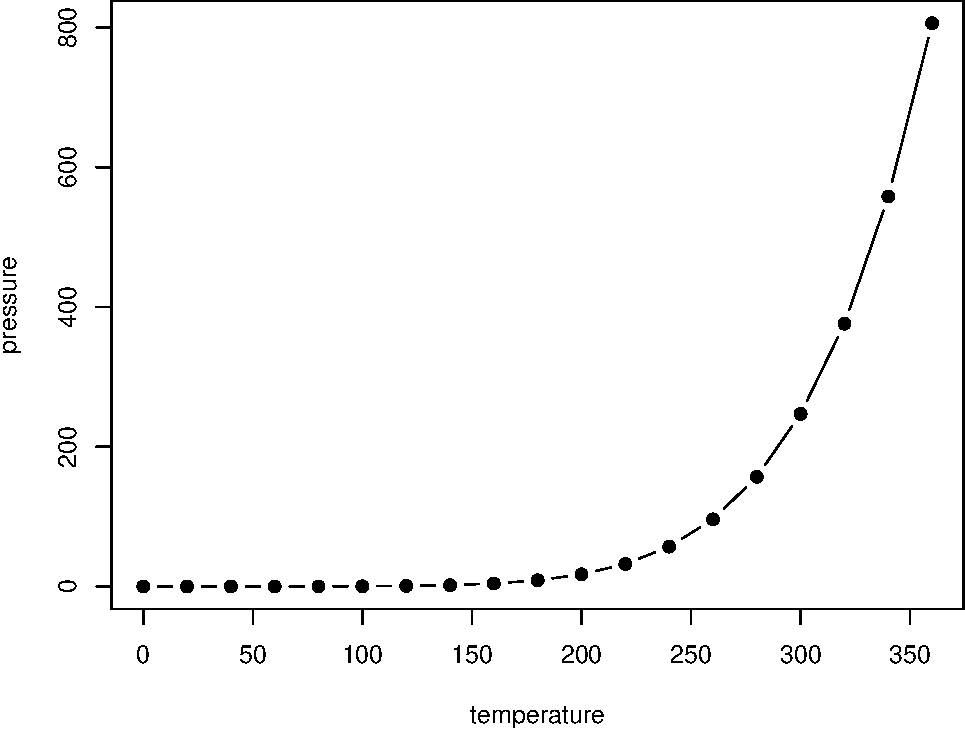
\includegraphics[width=0.8\linewidth]{01-intro_files/figure-latex/nice-fig-1} 

}

\caption{Here is a nice figure!}\label{fig:nice-fig}
\end{figure}

Reference a figure by its code chunk label with the \texttt{fig:} prefix, e.g., see Figure \texttt{\textbackslash{}@ref(fig:nice-fig)}. Similarly, you can reference tables generated from \texttt{knitr::kable()}, e.g., see Table \texttt{\textbackslash{}@ref(tab:nice-tab)}.

\begin{Shaded}
\begin{Highlighting}[]
\NormalTok{knitr}\SpecialCharTok{::}\FunctionTok{kable}\NormalTok{(}
  \FunctionTok{head}\NormalTok{(iris, }\DecValTok{20}\NormalTok{), }\AttributeTok{caption =} \StringTok{\textquotesingle{}Here is a nice table!\textquotesingle{}}\NormalTok{,}
  \AttributeTok{booktabs =} \ConstantTok{TRUE}
\NormalTok{)}
\end{Highlighting}
\end{Shaded}

\begin{table}

\caption{\label{tab:nice-tab}Here is a nice table!}
\centering
\begin{tabular}[t]{rrrrl}
\toprule
Sepal.Length & Sepal.Width & Petal.Length & Petal.Width & Species\\
\midrule
5.1 & 3.5 & 1.4 & 0.2 & setosa\\
4.9 & 3.0 & 1.4 & 0.2 & setosa\\
4.7 & 3.2 & 1.3 & 0.2 & setosa\\
4.6 & 3.1 & 1.5 & 0.2 & setosa\\
5.0 & 3.6 & 1.4 & 0.2 & setosa\\
\addlinespace
5.4 & 3.9 & 1.7 & 0.4 & setosa\\
4.6 & 3.4 & 1.4 & 0.3 & setosa\\
5.0 & 3.4 & 1.5 & 0.2 & setosa\\
4.4 & 2.9 & 1.4 & 0.2 & setosa\\
4.9 & 3.1 & 1.5 & 0.1 & setosa\\
\addlinespace
5.4 & 3.7 & 1.5 & 0.2 & setosa\\
4.8 & 3.4 & 1.6 & 0.2 & setosa\\
4.8 & 3.0 & 1.4 & 0.1 & setosa\\
4.3 & 3.0 & 1.1 & 0.1 & setosa\\
5.8 & 4.0 & 1.2 & 0.2 & setosa\\
\addlinespace
5.7 & 4.4 & 1.5 & 0.4 & setosa\\
5.4 & 3.9 & 1.3 & 0.4 & setosa\\
5.1 & 3.5 & 1.4 & 0.3 & setosa\\
5.7 & 3.8 & 1.7 & 0.3 & setosa\\
5.1 & 3.8 & 1.5 & 0.3 & setosa\\
\bottomrule
\end{tabular}
\end{table}

\hypertarget{citations}{%
\subsection{Citations}\label{citations}}

You can write citations, too. For example, we are using the \textbf{bookdown} package \citep{R-bookdown} in this sample book, which was built on top of R Markdown and \textbf{knitr} \citep{xie2015}.

\hypertarget{snippets}{%
\chapter{Snippets}\label{snippets}}

Random useful snippets that do not fit anywhere else.

\hypertarget{useful-rstudio-functions}{%
\section{Useful RStudio functions}\label{useful-rstudio-functions}}

\hypertarget{clean-restart}{%
\subsection{Clean restart}\label{clean-restart}}

Cleans current environment and restarts R session (no code can run past this). Indicate objects to leave alone by supplying string to \texttt{leave} argument.

\begin{Shaded}
\begin{Highlighting}[]
\NormalTok{clean\_restart }\OtherTok{=} \ControlFlowTok{function}\NormalTok{(}\AttributeTok{leave =} \ConstantTok{NULL}\NormalTok{)\{}
  \FunctionTok{rm}\NormalTok{(}\AttributeTok{list=}\FunctionTok{setdiff}\NormalTok{(}\FunctionTok{ls}\NormalTok{(}\AttributeTok{envir =}\NormalTok{ .GlobalEnv), leave), }\AttributeTok{envir =}\NormalTok{ .GlobalEnv)}
  \FunctionTok{invisible}\NormalTok{(}\FunctionTok{.rs.restartR}\NormalTok{())}
\NormalTok{\}}
\end{Highlighting}
\end{Shaded}

\hypertarget{remove-duplicated-packages-between-personal-and-system-libraries}{%
\subsection{Remove duplicated packages between personal and system libraries}\label{remove-duplicated-packages-between-personal-and-system-libraries}}

This removes any user library packages that are also present in the system library. Use this to minimise loading conflicts. Change \texttt{tdrake} in example to your rstudio username.

\begin{Shaded}
\begin{Highlighting}[]
\FunctionTok{library}\NormalTok{(tidyverse)}

\NormalTok{tdrake\_packages }\OtherTok{=} \FunctionTok{installed.packages}\NormalTok{() }\SpecialCharTok{\%\textgreater{}\%} \CommentTok{\#change \textquotesingle{}tdrake\textquotesingle{} to your rstudio username}
  \FunctionTok{as\_tibble}\NormalTok{() }\SpecialCharTok{\%\textgreater{}\%} 
  \FunctionTok{filter}\NormalTok{(LibPath }\SpecialCharTok{\%\textgreater{}\%} \FunctionTok{str\_detect}\NormalTok{(}\StringTok{"tdrake"}\NormalTok{)) }\SpecialCharTok{\%\textgreater{}\%} 
  \FunctionTok{pull}\NormalTok{(Package)}

\NormalTok{system\_packages }\OtherTok{=} \FunctionTok{installed.packages}\NormalTok{() }\SpecialCharTok{\%\textgreater{}\%} 
  \FunctionTok{as\_tibble}\NormalTok{() }\SpecialCharTok{\%\textgreater{}\%} 
  \FunctionTok{filter}\NormalTok{(LibPath }\SpecialCharTok{\%\textgreater{}\%} \FunctionTok{str\_detect}\NormalTok{(}\StringTok{"local"}\NormalTok{)) }\SpecialCharTok{\%\textgreater{}\%} 
  \FunctionTok{pull}\NormalTok{(Package)}

\NormalTok{to\_remove }\OtherTok{=}\NormalTok{ tdrake\_packages[tdrake\_packages }\SpecialCharTok{\%in\%}\NormalTok{ system\_packages]}

\FunctionTok{remove.packages}\NormalTok{(to\_remove)}
\ErrorTok{\}}
\end{Highlighting}
\end{Shaded}

\hypertarget{remove-large-file-accidentally-committed-to-git}{%
\subsection{Remove large file accidentally committed to git}\label{remove-large-file-accidentally-committed-to-git}}

\texttt{git\ filter-branch\ -f\ -\/-index-filter\ "git\ rm\ -rf\ -\/-cached\ -\/-ignore-unmatch\ filename.rda"\ HEAD}.

\hypertarget{memory-and-efficient-ram-usage}{%
\section{Memory and efficient RAM usage}\label{memory-and-efficient-ram-usage}}

\begin{enumerate}
\def\labelenumi{\arabic{enumi}.}
\tightlist
\item
  Restart R often
\item
  Use \texttt{rm(...)} to get rid of big files after using them
\item
  Save large objects (and compress with ``gz'') that take a while to create but are needed often (\texttt{write\_rds(x,\ "big\_file.rds.gz",\ compress\ =\ "gz)})
\item
  Run \texttt{gc()} (garbage collect)
\item
  Check memory usage: \texttt{pryr::mem\_used()}
\end{enumerate}

Most importantly if using big files (even if they aren't loaded in your environment!) do the following:

\begin{enumerate}
\def\labelenumi{\arabic{enumi}.}
\tightlist
\item
  \texttt{save.image("temp.rda")}
\item
  Restart R
\item
  \texttt{load("temp.rda")}
\item
  Delete ``temp.rda'' from \texttt{Files} pane
\end{enumerate}

\hypertarget{exporting-tables-that-work-in-both-pdf-and-word}{%
\section{Exporting tables that work in both PDF and Word}\label{exporting-tables-that-work-in-both-pdf-and-word}}

The \texttt{kable()} function from \texttt{library(knitr)} formats tables for all 3 output formats, but it is a bit limited.
\texttt{library(kableExtra)} is great for table customisations that work in PDF and HTML.
\texttt{kableExtra} functions do not work for Word output, but \texttt{library(flextable)} does work for Word (but not for PDF).

We can define our own table printing function that uses kableExtra or flextable based on output type:

\begin{Shaded}
\begin{Highlighting}[]
\CommentTok{\# This makes table resize or continue over multiple pages in all output types}
\CommentTok{\# PDF powered by kableExtra, Word by flextable}
\NormalTok{mytable }\OtherTok{=} \ControlFlowTok{function}\NormalTok{(x, }\AttributeTok{caption =} \StringTok{""}\NormalTok{, }\AttributeTok{longtable =} \ConstantTok{FALSE}\NormalTok{, ...)\{}
  \FunctionTok{library}\NormalTok{(kableExtra)}
  \CommentTok{\# if not latex or html then else is Word}
  \ControlFlowTok{if}\NormalTok{ (knitr}\SpecialCharTok{::}\FunctionTok{is\_latex\_output}\NormalTok{() }\SpecialCharTok{|}\NormalTok{ knitr}\SpecialCharTok{::}\FunctionTok{is\_html\_output}\NormalTok{())\{}
\NormalTok{    knitr}\SpecialCharTok{::}\FunctionTok{kable}\NormalTok{(x, }\AttributeTok{row.names =} \ConstantTok{FALSE}\NormalTok{, }\AttributeTok{align =} \FunctionTok{c}\NormalTok{(}\StringTok{"l"}\NormalTok{, }\StringTok{"l"}\NormalTok{, }\StringTok{"r"}\NormalTok{, }\StringTok{"r"}\NormalTok{, }\StringTok{"r"}\NormalTok{, }\StringTok{"r"}\NormalTok{, }\StringTok{"r"}\NormalTok{, }\StringTok{"r"}\NormalTok{, }\StringTok{"r"}\NormalTok{), }
          \AttributeTok{booktabs =} \ConstantTok{TRUE}\NormalTok{, }\AttributeTok{caption =}\NormalTok{ caption, }\AttributeTok{longtable =}\NormalTok{ longtable,}
          \AttributeTok{linesep =} \StringTok{""}\NormalTok{, ...) }\SpecialCharTok{\%\textgreater{}\%}
\NormalTok{    kableExtra}\SpecialCharTok{::}\FunctionTok{kable\_styling}\NormalTok{(}\AttributeTok{latex\_options =} \FunctionTok{c}\NormalTok{(}\StringTok{"scale\_down"}\NormalTok{, }\StringTok{"hold\_position"}\NormalTok{))}
\NormalTok{  \}}\ControlFlowTok{else}\NormalTok{\{}
\NormalTok{    flextable}\SpecialCharTok{::}\FunctionTok{flextable}\NormalTok{(x) }\SpecialCharTok{\%\textgreater{}\%} 
\NormalTok{      flextable}\SpecialCharTok{::}\FunctionTok{autofit}\NormalTok{() }\SpecialCharTok{\%\textgreater{}\%} 
\NormalTok{      flextable}\SpecialCharTok{::}\FunctionTok{width}\NormalTok{(}\AttributeTok{j =} \DecValTok{1}\NormalTok{, }\AttributeTok{width =} \FloatTok{1.5}\NormalTok{) }\SpecialCharTok{\%\textgreater{}\%} 
\NormalTok{      flextable}\SpecialCharTok{::}\FunctionTok{height}\NormalTok{(}\AttributeTok{i =} \DecValTok{1}\NormalTok{, }\AttributeTok{height =} \FloatTok{0.5}\NormalTok{, }\AttributeTok{part =} \StringTok{"header"}\NormalTok{)}
\NormalTok{  \}}
  
\NormalTok{\}}
\FunctionTok{library}\NormalTok{(dplyr)}
\NormalTok{cars }\SpecialCharTok{\%\textgreater{}\%} 
  \FunctionTok{head}\NormalTok{() }\SpecialCharTok{\%\textgreater{}\%} 
  \FunctionTok{mytable}\NormalTok{()}
\end{Highlighting}
\end{Shaded}

\begin{table}[!h]

\caption{\label{tab:unnamed-chunk-3}}
\centering
\resizebox{\linewidth}{!}{
\begin{tabular}[t]{ll}
\toprule
speed & dist\\
\midrule
4 & 2\\
4 & 10\\
7 & 4\\
7 & 22\\
8 & 16\\
9 & 10\\
\bottomrule
\end{tabular}}
\end{table}

\hypertarget{warning-in-kableextra.-please-specify-format-in-kable.-kableextra-can-customize-either-html-or-latex-outputs.}{%
\subsection{Warning in kableExtra. Please specify format in kable. kableExtra can customize either HTML or LaTeX outputs.}\label{warning-in-kableextra.-please-specify-format-in-kable.-kableextra-can-customize-either-html-or-latex-outputs.}}

This warning goes away when you load \texttt{library(kableExtra)} in your script, instead of just using \texttt{kableExtra::function()}.

What happens when you load \texttt{library(kableExtra)} is that it sets that specifies the format for the R session, so that Warning goes away. It does mean that the \texttt{render()} function may fail since it knits in the same environment you have, rather than a new one like the Knit button does.

\hypertarget{creating-reproducible-r-examples-to-share-in-the-group-binder-holepunch-and-docker}{%
\section{Creating Reproducible R Examples to Share in the Group (binder, holepunch and docker)}\label{creating-reproducible-r-examples-to-share-in-the-group-binder-holepunch-and-docker}}

When asking for help with R code having a reproducible example is crucial (some mock data that others can use along with your code to reproduce your error). Often this can be done easily with creation of a small tibble and posting of the code on slack but sometimes it requires more complex data or the error is due to something in the Linux system in which RStudio server is hosted. For example if the \texttt{cairo} package for Linux isn't installed then plots don't work. The \texttt{holepunch} package helps to reproduce examples like these (not suitable for projects with confidential data).

\hypertarget{create-basic-reproducible-examples}{%
\subsection{Create Basic Reproducible Examples}\label{create-basic-reproducible-examples}}

The three main parts of the reproducible example (reprex) in Surgical Informatics are 1. packages, 2. small dataset and 3. code. Other things like R version and Linux version can be assumed as we all use one of only a few servers.

If you have a small (and confidential) set of data in a tibble or data frame called \texttt{my\_data} and want it to be easily copied run: \texttt{dput(droplevels(my\_data))}. This will print out code in the console that can be copy-pasted to reproduce the data frame. Alternatively use the \texttt{tibble} or \texttt{tribble} functions to create it from scratch (this is preferable for simple datasets). Then copy in the packages and finally the code (ideally the least amount possible to generate the error) and share with the group e.g.:

\begin{Shaded}
\begin{Highlighting}[]
\FunctionTok{library}\NormalTok{(tidyverse)}

\CommentTok{\# Output generated from dput(droplevels(my\_data))}
\NormalTok{data }\OtherTok{=} \FunctionTok{structure}\NormalTok{(}\FunctionTok{list}\NormalTok{(}\AttributeTok{a =} \FunctionTok{c}\NormalTok{(}\DecValTok{1}\NormalTok{, }\DecValTok{2}\NormalTok{, }\DecValTok{3}\NormalTok{), }\AttributeTok{b =} \FunctionTok{c}\NormalTok{(}\StringTok{"a"}\NormalTok{, }\StringTok{"b"}\NormalTok{, }\StringTok{"c"}\NormalTok{), }\AttributeTok{c =} \DecValTok{10}\SpecialCharTok{:}\DecValTok{12}\NormalTok{), }\AttributeTok{.Names =} \FunctionTok{c}\NormalTok{(}\StringTok{"a"}\NormalTok{, }
\StringTok{"b"}\NormalTok{, }\StringTok{"c"}\NormalTok{), }\AttributeTok{row.names =} \FunctionTok{c}\NormalTok{(}\ConstantTok{NA}\NormalTok{, }\SpecialCharTok{{-}}\NormalTok{3L), }\AttributeTok{class =} \FunctionTok{c}\NormalTok{(}\StringTok{"tbl\_df"}\NormalTok{, }\StringTok{"tbl"}\NormalTok{, }
\StringTok{"data.frame"}\NormalTok{))}

\NormalTok{data }\SpecialCharTok{\%\textgreater{}\%} 
  \FunctionTok{mutate}\NormalTok{(}\AttributeTok{newvar =}\NormalTok{ a }\SpecialCharTok{/}\NormalTok{b)}
\end{Highlighting}
\end{Shaded}

\begin{verbatim}
## Error in `mutate()`:
## ! Problem while computing `newvar = a/b`.
## Caused by error in `a / b`:
## ! non-numeric argument to binary operator
\end{verbatim}

\hypertarget{holepunch---complex-reproducible-examples}{%
\subsection{\texorpdfstring{\texttt{holepunch} - Complex Reproducible Examples}{holepunch - Complex Reproducible Examples}}\label{holepunch---complex-reproducible-examples}}

From your project with data you are happy to make public make sure you are backed up to \texttt{git} and \texttt{GitHub}. See the relevant chapter on how to do this. Then run the following:

\begin{Shaded}
\begin{Highlighting}[]
\CommentTok{\# Holepunch testing}

\NormalTok{remotes}\SpecialCharTok{::}\FunctionTok{install\_github}\NormalTok{(}\StringTok{"karthik/holepunch"}\NormalTok{)}

\FunctionTok{library}\NormalTok{(holepunch)}
\FunctionTok{write\_compendium\_description}\NormalTok{(}\AttributeTok{package =} \StringTok{"Title of my project"}\NormalTok{, }
                             \AttributeTok{description =} \StringTok{"Rough description of project or issue"}\NormalTok{)}

\FunctionTok{write\_dockerfile}\NormalTok{(}\AttributeTok{maintainer =} \StringTok{"SurgicalInformatics"}\NormalTok{)}

\FunctionTok{generate\_badge}\NormalTok{()}

\FunctionTok{build\_binder}\NormalTok{()}
\end{Highlighting}
\end{Shaded}

The file will generate some text to copy into the top of a \texttt{README.md} file. It will look like:

\begin{Shaded}
\begin{Highlighting}[]
\SpecialCharTok{\textless{}!{-}{-}}\NormalTok{ badges}\SpecialCharTok{:}\NormalTok{ start }\SpecialCharTok{{-}}\OtherTok{{-}\textgreater{}}
\NormalTok{[}\SpecialCharTok{!}\NormalTok{[Launch Rstudio Binder](http}\SpecialCharTok{:}\ErrorTok{//}\NormalTok{mybinder.org}\SpecialCharTok{/}\NormalTok{badge\_logo.svg)](https}\SpecialCharTok{:}\ErrorTok{//}\NormalTok{mybinder.org}\SpecialCharTok{/}\NormalTok{v2}\SpecialCharTok{/}\NormalTok{gh}\SpecialCharTok{/}\NormalTok{SurgicalInformatics}\SpecialCharTok{/}\ErrorTok{\textless{}}\NormalTok{project}\SpecialCharTok{\textgreater{}}\ErrorTok{/}\NormalTok{master?}\AttributeTok{urlpath=}\NormalTok{rstudio)}
\SpecialCharTok{\textless{}!{-}{-}}\NormalTok{ badges}\SpecialCharTok{:}\NormalTok{ end }\SpecialCharTok{{-}}\OtherTok{{-}\textgreater{}}
\end{Highlighting}
\end{Shaded}

Now, whenever somebody clicks on the badge in the \texttt{README} on \texttt{GitHub} they will be taken to an RStudio server instance with all your files (excluding files listed in \texttt{.gitignore}), all the current versions of your package, all the current Linux packages and the current R version. They can then test your code in an near-identical environment to help identify the source of the error, their session will time out after 10 minutes of inactivity or 12 hours since starting and will not save anything so should only be used for bug-testing or quick examples.

As this is a free version of RStudio server there is a limit to what is supported and it shouldn't be used for computationally-intensive processes.

And, as mentioned: \textbf{No confidential data.}

\hypertarget{working-with-chis}{%
\section{Working with CHIs}\label{working-with-chis}}

Here are 4 functions for CHIs that could even be put in a small package.
The Community Health Index (CHI) is a population register, which is used in Scotland for health care purposes.
The CHI number uniquely identifies a person on the index.

\hypertarget{chi_dob---extract-date-of-birth-from-chi}{%
\subsection{\texorpdfstring{\texttt{chi\_dob()} - Extract date of birth from CHI}{chi\_dob() - Extract date of birth from CHI}}\label{chi_dob---extract-date-of-birth-from-chi}}

Note \texttt{cutoff\_2000}.
As CHI has only a two digit year, need to decide whether year is 1900s or 2000s.
I don't think there is a formal way of determining this.

\begin{Shaded}
\begin{Highlighting}[]
\FunctionTok{library}\NormalTok{(dplyr)}
\NormalTok{chi }\OtherTok{=} \FunctionTok{c}\NormalTok{(}\StringTok{"1009701234"}\NormalTok{, }\StringTok{"1811431232"}\NormalTok{, }\StringTok{"1304496368"}\NormalTok{)}
\CommentTok{\# These CHIs are not real. }
\CommentTok{\# The first is invalid, two and three are valid. }

\CommentTok{\# Cut{-}off any thing before that number is considered 2000s}
\CommentTok{\# i.e. at cutoff\_2000 = 20, "18" is considered 2018, rather than 1918. }
\NormalTok{chi\_dob }\OtherTok{=} \ControlFlowTok{function}\NormalTok{(.data, }\AttributeTok{cutoff\_2000 =} \DecValTok{20}\NormalTok{)\{}
\NormalTok{  .data }\SpecialCharTok{\%\textgreater{}\%} 
\NormalTok{    stringr}\SpecialCharTok{::}\FunctionTok{str\_extract}\NormalTok{(}\StringTok{".\{6\}"}\NormalTok{) }\SpecialCharTok{\%\textgreater{}\%} 
\NormalTok{    lubridate}\SpecialCharTok{::}\FunctionTok{parse\_date\_time2}\NormalTok{(}\StringTok{"dmy"}\NormalTok{, }\AttributeTok{cutoff\_2000 =}\NormalTok{ cutoff\_2000) }\SpecialCharTok{\%\textgreater{}\%} 
\NormalTok{    lubridate}\SpecialCharTok{::}\FunctionTok{as\_date}\NormalTok{() }\CommentTok{\# Make Date object, rather than POSIXct}
\NormalTok{\}}

\FunctionTok{chi\_dob}\NormalTok{(chi)}
\end{Highlighting}
\end{Shaded}

\begin{verbatim}
## [1] "1970-09-10" "1943-11-18" "1949-04-13"
\end{verbatim}

\begin{Shaded}
\begin{Highlighting}[]
\CommentTok{\# From tibble}
\FunctionTok{tibble}\NormalTok{(}\AttributeTok{chi =}\NormalTok{ chi) }\SpecialCharTok{\%\textgreater{}\%} 
  \FunctionTok{mutate}\NormalTok{(}
    \AttributeTok{dob =} \FunctionTok{chi\_dob}\NormalTok{(chi)}
\NormalTok{  )}
\end{Highlighting}
\end{Shaded}

\begin{verbatim}
## # A tibble: 3 x 2
##   chi        dob       
##   <chr>      <date>    
## 1 1009701234 1970-09-10
## 2 1811431232 1943-11-18
## 3 1304496368 1949-04-13
\end{verbatim}

\hypertarget{chi_gender---extract-gender-from-chi}{%
\subsection{\texorpdfstring{\texttt{chi\_gender()} - Extract gender from CHI}{chi\_gender() - Extract gender from CHI}}\label{chi_gender---extract-gender-from-chi}}

Ninth digit is odd for men and even for women.
A test for even is \texttt{x\ modulus\ 2\ ==\ 0}.

\begin{Shaded}
\begin{Highlighting}[]
\NormalTok{chi\_gender }\OtherTok{=} \ControlFlowTok{function}\NormalTok{(.data)\{}
\NormalTok{  .data }\SpecialCharTok{\%\textgreater{}\%} 
\NormalTok{    stringr}\SpecialCharTok{::}\FunctionTok{str\_sub}\NormalTok{(}\DecValTok{9}\NormalTok{, }\DecValTok{9}\NormalTok{) }\SpecialCharTok{\%\textgreater{}\%} 
    \FunctionTok{as.numeric}\NormalTok{() }\SpecialCharTok{\%\textgreater{}\%} 
\NormalTok{    \{}\FunctionTok{ifelse}\NormalTok{(. }\SpecialCharTok{\%\%} \DecValTok{2} \SpecialCharTok{==} \DecValTok{0}\NormalTok{, }\StringTok{"Female"}\NormalTok{, }\StringTok{"Male"}\NormalTok{)\}}
\NormalTok{\}}

\FunctionTok{chi\_gender}\NormalTok{(chi)}
\end{Highlighting}
\end{Shaded}

\begin{verbatim}
## [1] "Male"   "Male"   "Female"
\end{verbatim}

\begin{Shaded}
\begin{Highlighting}[]
\CommentTok{\# From tibble}
\FunctionTok{tibble}\NormalTok{(}\AttributeTok{chi =}\NormalTok{ chi) }\SpecialCharTok{\%\textgreater{}\%} 
  \FunctionTok{mutate}\NormalTok{(}
    \AttributeTok{dob =} \FunctionTok{chi\_dob}\NormalTok{(chi),}
    \AttributeTok{gender =} \FunctionTok{chi\_gender}\NormalTok{(chi)}
\NormalTok{  )}
\end{Highlighting}
\end{Shaded}

\begin{verbatim}
## # A tibble: 3 x 3
##   chi        dob        gender
##   <chr>      <date>     <chr> 
## 1 1009701234 1970-09-10 Male  
## 2 1811431232 1943-11-18 Male  
## 3 1304496368 1949-04-13 Female
\end{verbatim}

\hypertarget{chi_age---extract-age-from-chi}{%
\subsection{\texorpdfstring{\texttt{chi\_age()} - Extract age from CHI}{chi\_age() - Extract age from CHI}}\label{chi_age---extract-age-from-chi}}

Works for a single date or a vector of dates.

\begin{Shaded}
\begin{Highlighting}[]
\NormalTok{chi\_age }\OtherTok{=} \ControlFlowTok{function}\NormalTok{(.data, ref\_date, }\AttributeTok{cutoff\_2000 =} \DecValTok{20}\NormalTok{)\{}
\NormalTok{  dob }\OtherTok{=} \FunctionTok{chi\_dob}\NormalTok{(.data, }\AttributeTok{cutoff\_2000 =}\NormalTok{ cutoff\_2000)}
\NormalTok{  lubridate}\SpecialCharTok{::}\FunctionTok{interval}\NormalTok{(dob, ref\_date) }\SpecialCharTok{\%\textgreater{}\%} 
    \FunctionTok{as.numeric}\NormalTok{(}\StringTok{"years"}\NormalTok{) }\SpecialCharTok{\%\textgreater{}\%} 
    \FunctionTok{floor}\NormalTok{()}
\NormalTok{\}}

\CommentTok{\# Today}
\FunctionTok{chi\_age}\NormalTok{(chi, }\FunctionTok{Sys.time}\NormalTok{())}
\end{Highlighting}
\end{Shaded}

\begin{verbatim}
## [1] 51 78 73
\end{verbatim}

\begin{Shaded}
\begin{Highlighting}[]
\CommentTok{\# Single date}
\FunctionTok{library}\NormalTok{(lubridate)}
\FunctionTok{chi\_age}\NormalTok{(chi, }\FunctionTok{dmy}\NormalTok{(}\StringTok{"11/09/2018"}\NormalTok{))}
\end{Highlighting}
\end{Shaded}

\begin{verbatim}
## [1] 48 74 69
\end{verbatim}

\begin{Shaded}
\begin{Highlighting}[]
\CommentTok{\# Vector}
\NormalTok{dates }\OtherTok{=} \FunctionTok{dmy}\NormalTok{(}\StringTok{"11/09/2018"}\NormalTok{,}
            \StringTok{"09/05/2015"}\NormalTok{,}
            \StringTok{"10/03/2014"}\NormalTok{)}
\FunctionTok{chi\_age}\NormalTok{(chi, dates)}
\end{Highlighting}
\end{Shaded}

\begin{verbatim}
## [1] 48 71 64
\end{verbatim}

\begin{Shaded}
\begin{Highlighting}[]
\CommentTok{\# From tibble}
\FunctionTok{tibble}\NormalTok{(}\AttributeTok{chi =}\NormalTok{ chi) }\SpecialCharTok{\%\textgreater{}\%} 
  \FunctionTok{mutate}\NormalTok{(}
    \AttributeTok{dob =} \FunctionTok{chi\_dob}\NormalTok{(chi),}
    \AttributeTok{gender =} \FunctionTok{chi\_gender}\NormalTok{(chi),}
    \AttributeTok{age =} \FunctionTok{chi\_age}\NormalTok{(chi, }\FunctionTok{Sys.time}\NormalTok{())}
\NormalTok{  )}
\end{Highlighting}
\end{Shaded}

\begin{verbatim}
## # A tibble: 3 x 4
##   chi        dob        gender   age
##   <chr>      <date>     <chr>  <dbl>
## 1 1009701234 1970-09-10 Male      51
## 2 1811431232 1943-11-18 Male      78
## 3 1304496368 1949-04-13 Female    73
\end{verbatim}

\hypertarget{chi_valid---logical-test-for-valid-chi}{%
\subsection{\texorpdfstring{\texttt{chi\_valid()} - Logical test for valid CHI}{chi\_valid() - Logical test for valid CHI}}\label{chi_valid---logical-test-for-valid-chi}}

The final digit of the CHI can be used to test that the number is correct via the modulus 11 algorithm.

\begin{Shaded}
\begin{Highlighting}[]
\NormalTok{chi\_valid }\OtherTok{=} \ControlFlowTok{function}\NormalTok{(.data)\{}
\NormalTok{  .data }\SpecialCharTok{\%\textgreater{}\%} 
\NormalTok{    stringr}\SpecialCharTok{::}\FunctionTok{str\_split}\NormalTok{(}\StringTok{""}\NormalTok{, }\AttributeTok{simplify =} \ConstantTok{TRUE}\NormalTok{) }\SpecialCharTok{\%\textgreater{}\%} 
\NormalTok{    .[, }\SpecialCharTok{{-}}\DecValTok{10}\NormalTok{] }\SpecialCharTok{\%\textgreater{}\%}              \CommentTok{\# Working with matrices hence brackets}
    \FunctionTok{apply}\NormalTok{(}\DecValTok{1}\NormalTok{, as.numeric) }\SpecialCharTok{\%\textgreater{}\%}  \CommentTok{\# Convert from string}
\NormalTok{    \{}\FunctionTok{seq}\NormalTok{(}\DecValTok{10}\NormalTok{, }\DecValTok{2}\NormalTok{) }\SpecialCharTok{\%*\%}\NormalTok{ .\} }\SpecialCharTok{\%\textgreater{}\%}    \CommentTok{\# Multiply and sum step}
\NormalTok{    \{. }\SpecialCharTok{\%\%} \DecValTok{11}\NormalTok{\} }\SpecialCharTok{\%\textgreater{}\%}             \CommentTok{\# Modulus 11}
\NormalTok{    \{}\DecValTok{11} \SpecialCharTok{{-}}\NormalTok{ .\} }\SpecialCharTok{\%\textgreater{}\%}              \CommentTok{\# Substract from 11}
\NormalTok{    dplyr}\SpecialCharTok{::}\FunctionTok{near}\NormalTok{(              }\CommentTok{\# Compare result with 10th digit. }
\NormalTok{      \{stringr}\SpecialCharTok{::}\FunctionTok{str\_sub}\NormalTok{(chi, }\DecValTok{10}\NormalTok{) }\SpecialCharTok{\%\textgreater{}\%} \FunctionTok{as.numeric}\NormalTok{()\}}
\NormalTok{    ) }\SpecialCharTok{\%\textgreater{}\%} 
    \FunctionTok{as.vector}\NormalTok{()}
\NormalTok{\}}

\FunctionTok{chi\_valid}\NormalTok{(chi)}
\end{Highlighting}
\end{Shaded}

\begin{verbatim}
## [1] FALSE  TRUE  TRUE
\end{verbatim}

\begin{Shaded}
\begin{Highlighting}[]
\CommentTok{\# From tibble}
\FunctionTok{tibble}\NormalTok{(}\AttributeTok{chi =}\NormalTok{ chi) }\SpecialCharTok{\%\textgreater{}\%} 
  \FunctionTok{mutate}\NormalTok{(}
    \AttributeTok{dob =} \FunctionTok{chi\_dob}\NormalTok{(chi),}
    \AttributeTok{gender =} \FunctionTok{chi\_gender}\NormalTok{(chi),}
    \AttributeTok{age =} \FunctionTok{chi\_age}\NormalTok{(chi, }\FunctionTok{Sys.time}\NormalTok{()),}
    \AttributeTok{chi\_valid =} \FunctionTok{chi\_valid}\NormalTok{(chi)}
\NormalTok{  )}
\end{Highlighting}
\end{Shaded}

\begin{verbatim}
## # A tibble: 3 x 5
##   chi        dob        gender   age chi_valid
##   <chr>      <date>     <chr>  <dbl> <lgl>    
## 1 1009701234 1970-09-10 Male      51 FALSE    
## 2 1811431232 1943-11-18 Male      78 TRUE     
## 3 1304496368 1949-04-13 Female    73 TRUE
\end{verbatim}

\hypertarget{working-with-dates}{%
\section{Working with dates}\label{working-with-dates}}

\hypertarget{difference-between-two-dates}{%
\subsection{Difference between two dates}\label{difference-between-two-dates}}

I always forget how to do this neatly.
I often want days as a numeric, not a lubridate type object.

\begin{Shaded}
\begin{Highlighting}[]
\FunctionTok{library}\NormalTok{(lubridate)}
\NormalTok{date1 }\OtherTok{=} \FunctionTok{dmy}\NormalTok{(}\StringTok{"12/03/2018"}\NormalTok{, }\StringTok{"14/05/2017"}\NormalTok{)}
\NormalTok{date2 }\OtherTok{=} \FunctionTok{dmy}\NormalTok{(}\StringTok{"11/09/2019"}\NormalTok{, }\StringTok{"11/04/2019"}\NormalTok{)}

\FunctionTok{interval}\NormalTok{(date1, date2) }\SpecialCharTok{\%\textgreater{}\%} 
  \FunctionTok{as.numeric}\NormalTok{(}\StringTok{"days"}\NormalTok{)}
\end{Highlighting}
\end{Shaded}

\begin{verbatim}
## [1] 548 697
\end{verbatim}

\hypertarget{lags}{%
\subsection{Lags}\label{lags}}

This is useful for calculating, for instance, the period off medications. Lags are much better than long to wide solutions for this.

\begin{Shaded}
\begin{Highlighting}[]
\FunctionTok{library}\NormalTok{(tidyverse)}
\FunctionTok{library}\NormalTok{(lubridate)}
\NormalTok{id }\OtherTok{=} \FunctionTok{c}\NormalTok{(}\DecValTok{2}\NormalTok{, }\DecValTok{2}\NormalTok{, }\DecValTok{2}\NormalTok{, }\DecValTok{2}\NormalTok{, }\DecValTok{3}\NormalTok{, }\DecValTok{5}\NormalTok{) }
\NormalTok{medication }\OtherTok{=} \FunctionTok{c}\NormalTok{(}\StringTok{"aspirin"}\NormalTok{, }\StringTok{"aspirin"}\NormalTok{, }\StringTok{"aspirin"}\NormalTok{, }\StringTok{"tylenol"}\NormalTok{, }\StringTok{"lipitor"}\NormalTok{, }\StringTok{"advil"}\NormalTok{) }
\NormalTok{start.date }\OtherTok{=} \FunctionTok{c}\NormalTok{(}\StringTok{"05/01/2017"}\NormalTok{, }\StringTok{"05/30/2017"}\NormalTok{, }\StringTok{"07/15/2017"}\NormalTok{, }\StringTok{"05/01/2017"}\NormalTok{, }\StringTok{"05/06/2017"}\NormalTok{, }\StringTok{"05/28/2017"}\NormalTok{)}
\NormalTok{stop.date }\OtherTok{=} \FunctionTok{c}\NormalTok{(}\StringTok{"05/04/2017"}\NormalTok{, }\StringTok{"06/10/2017"}\NormalTok{, }\StringTok{"07/27/2017"}\NormalTok{, }\StringTok{"05/15/2017"}\NormalTok{, }\StringTok{"05/12/2017"}\NormalTok{, }\StringTok{"06/13/2017"}\NormalTok{)}
\NormalTok{df }\OtherTok{=} \FunctionTok{tibble}\NormalTok{(id, medication, start.date, stop.date)}
\NormalTok{df}
\end{Highlighting}
\end{Shaded}

\begin{verbatim}
## # A tibble: 6 x 4
##      id medication start.date stop.date 
##   <dbl> <chr>      <chr>      <chr>     
## 1     2 aspirin    05/01/2017 05/04/2017
## 2     2 aspirin    05/30/2017 06/10/2017
## 3     2 aspirin    07/15/2017 07/27/2017
## 4     2 tylenol    05/01/2017 05/15/2017
## 5     3 lipitor    05/06/2017 05/12/2017
## 6     5 advil      05/28/2017 06/13/2017
\end{verbatim}

\begin{Shaded}
\begin{Highlighting}[]
\NormalTok{df }\SpecialCharTok{\%\textgreater{}\%}
  \FunctionTok{mutate\_at}\NormalTok{(}\FunctionTok{c}\NormalTok{(}\StringTok{"start.date"}\NormalTok{, }\StringTok{"stop.date"}\NormalTok{), lubridate}\SpecialCharTok{::}\NormalTok{mdy) }\SpecialCharTok{\%\textgreater{}\%} \CommentTok{\# make a date}
  \FunctionTok{arrange}\NormalTok{(id, medication, start.date) }\SpecialCharTok{\%\textgreater{}\%} 
  \FunctionTok{group\_by}\NormalTok{(id, medication) }\SpecialCharTok{\%\textgreater{}\%} 
  \FunctionTok{mutate}\NormalTok{(}
    \AttributeTok{start\_date\_diff =}\NormalTok{ start.date }\SpecialCharTok{{-}} \FunctionTok{lag}\NormalTok{(start.date),}
    \AttributeTok{medication\_period =}\NormalTok{ stop.date}\SpecialCharTok{{-}}\NormalTok{start.date}
\NormalTok{  )}
\end{Highlighting}
\end{Shaded}

\begin{verbatim}
## # A tibble: 6 x 6
## # Groups:   id, medication [4]
##      id medication start.date stop.date  start_date_diff medication_period
##   <dbl> <chr>      <date>     <date>     <drtn>          <drtn>           
## 1     2 aspirin    2017-05-01 2017-05-04 NA days          3 days          
## 2     2 aspirin    2017-05-30 2017-06-10 29 days         11 days          
## 3     2 aspirin    2017-07-15 2017-07-27 46 days         12 days          
## 4     2 tylenol    2017-05-01 2017-05-15 NA days         14 days          
## 5     3 lipitor    2017-05-06 2017-05-12 NA days          6 days          
## 6     5 advil      2017-05-28 2017-06-13 NA days         16 days
\end{verbatim}

\hypertarget{pulling-out-change-in-status-data}{%
\subsection{Pulling out ``change in status'' data}\label{pulling-out-change-in-status-data}}

If you have a number of episodes per patient, each with a status and a time, then you need to do this as a starting point for CPH analysis.

\hypertarget{guess-the-format-of-dates}{%
\subsection{Guess the Format of Dates}\label{guess-the-format-of-dates}}

This function helps guess the date format from a dataset you have received. Add in new formats (as per lubridate) if they don't match. Once you work out what format it is then extract date with \texttt{mdy()} or \texttt{dmy()} etc. based on format.

\begin{Shaded}
\begin{Highlighting}[]
\FunctionTok{library}\NormalTok{(tidyverse)}
\FunctionTok{library}\NormalTok{(lubridate)}
\NormalTok{lakers }\OtherTok{=}\NormalTok{ lakers }\SpecialCharTok{\%\textgreater{}\%}
  \FunctionTok{mutate}\NormalTok{(}\AttributeTok{mm\_date =} \FunctionTok{paste0}\NormalTok{(}\FunctionTok{str\_sub}\NormalTok{(date, }\AttributeTok{start =}\DecValTok{5}\NormalTok{, }\AttributeTok{end =} \DecValTok{6}\NormalTok{), }\StringTok{"/"}\NormalTok{,}
                          \FunctionTok{str\_sub}\NormalTok{(date, }\AttributeTok{start =} \DecValTok{7}\NormalTok{, }\AttributeTok{end =} \DecValTok{8}\NormalTok{), }\StringTok{"/"}\NormalTok{,}
                          \FunctionTok{str\_sub}\NormalTok{(date, }\AttributeTok{start =} \DecValTok{1}\NormalTok{, }\AttributeTok{end =} \DecValTok{4}\NormalTok{)),}
         \AttributeTok{dd\_date =} \FunctionTok{paste0}\NormalTok{(}\FunctionTok{str\_sub}\NormalTok{(date, }\AttributeTok{start =}\DecValTok{7}\NormalTok{, }\AttributeTok{end =} \DecValTok{8}\NormalTok{), }\StringTok{"/"}\NormalTok{,}
                          \FunctionTok{str\_sub}\NormalTok{(date, }\AttributeTok{start =} \DecValTok{5}\NormalTok{, }\AttributeTok{end =} \DecValTok{6}\NormalTok{), }\StringTok{"/"}\NormalTok{,}
                          \FunctionTok{str\_sub}\NormalTok{(date, }\AttributeTok{start =} \DecValTok{1}\NormalTok{, }\AttributeTok{end =} \DecValTok{4}\NormalTok{)))}

\FunctionTok{guess\_formats}\NormalTok{(lakers}\SpecialCharTok{$}\NormalTok{mm\_date, }\FunctionTok{c}\NormalTok{(}\StringTok{"dmy"}\NormalTok{, }\StringTok{"mdy"}\NormalTok{), }\AttributeTok{print\_matches =} \ConstantTok{TRUE}\NormalTok{)}
\FunctionTok{guess\_formats}\NormalTok{(lakers}\SpecialCharTok{$}\NormalTok{dd\_date, }\FunctionTok{c}\NormalTok{(}\StringTok{"dmy"}\NormalTok{, }\StringTok{"mdy"}\NormalTok{), }\AttributeTok{print\_matches =} \ConstantTok{TRUE}\NormalTok{)}
\end{Highlighting}
\end{Shaded}

\hypertarget{example-data}{%
\subsubsection{Example data}\label{example-data}}

\begin{Shaded}
\begin{Highlighting}[]
\FunctionTok{library}\NormalTok{(dplyr)}
\FunctionTok{library}\NormalTok{(lubridate)}
\FunctionTok{library}\NormalTok{(finalfit)}
\NormalTok{mydata }\OtherTok{=} \FunctionTok{tibble}\NormalTok{(}
  \AttributeTok{id =} \FunctionTok{c}\NormalTok{(}\DecValTok{1}\NormalTok{,}\DecValTok{1}\NormalTok{,}\DecValTok{1}\NormalTok{,}\DecValTok{1}\NormalTok{,}\DecValTok{2}\NormalTok{,}\DecValTok{2}\NormalTok{,}\DecValTok{2}\NormalTok{,}\DecValTok{2}\NormalTok{,}\DecValTok{3}\NormalTok{,}\DecValTok{3}\NormalTok{,}\DecValTok{3}\NormalTok{,}\DecValTok{3}\NormalTok{,}\DecValTok{4}\NormalTok{,}\DecValTok{4}\NormalTok{,}\DecValTok{4}\NormalTok{,}\DecValTok{4}\NormalTok{,}\DecValTok{5}\NormalTok{,}\DecValTok{5}\NormalTok{,}\DecValTok{5}\NormalTok{,}\DecValTok{5}\NormalTok{),}
  \AttributeTok{status =} \FunctionTok{c}\NormalTok{(}\DecValTok{0}\NormalTok{,}\DecValTok{0}\NormalTok{,}\DecValTok{0}\NormalTok{,}\DecValTok{1}\NormalTok{,}\DecValTok{0}\NormalTok{,}\DecValTok{0}\NormalTok{,}\DecValTok{1}\NormalTok{,}\DecValTok{1}\NormalTok{,}\DecValTok{0}\NormalTok{,}\DecValTok{0}\NormalTok{,}\DecValTok{0}\NormalTok{,}\DecValTok{0}\NormalTok{,}\DecValTok{0}\NormalTok{,}\DecValTok{1}\NormalTok{,}\DecValTok{1}\NormalTok{,}\DecValTok{1}\NormalTok{,}\DecValTok{0}\NormalTok{,}\DecValTok{0}\NormalTok{,}\DecValTok{1}\NormalTok{,}\DecValTok{1}\NormalTok{),}
  \AttributeTok{group =} \FunctionTok{c}\NormalTok{(}\FunctionTok{rep}\NormalTok{(}\DecValTok{0}\NormalTok{, }\DecValTok{8}\NormalTok{), }\FunctionTok{rep}\NormalTok{(}\DecValTok{1}\NormalTok{, }\DecValTok{12}\NormalTok{)) }\SpecialCharTok{\%\textgreater{}\%} \FunctionTok{factor}\NormalTok{(),}
  \AttributeTok{opdate =} \FunctionTok{rep}\NormalTok{(}\StringTok{"2010/01/01"}\NormalTok{, }\DecValTok{20}\NormalTok{) }\SpecialCharTok{\%\textgreater{}\%} \FunctionTok{ymd}\NormalTok{(),}
  \AttributeTok{status\_date =} \FunctionTok{c}\NormalTok{(}
    \StringTok{"2010/02/01"}\NormalTok{, }\StringTok{"2010/03/01"}\NormalTok{, }\StringTok{"2010/04/01"}\NormalTok{, }\StringTok{"2010/05/01"}\NormalTok{,}
    \StringTok{"2010/02/02"}\NormalTok{, }\StringTok{"2010/03/02"}\NormalTok{, }\StringTok{"2010/04/02"}\NormalTok{, }\StringTok{"2010/05/02"}\NormalTok{,}
    \StringTok{"2010/02/03"}\NormalTok{, }\StringTok{"2010/03/03"}\NormalTok{, }\StringTok{"2010/04/03"}\NormalTok{, }\StringTok{"2010/05/03"}\NormalTok{,}
    \StringTok{"2010/02/04"}\NormalTok{, }\StringTok{"2010/03/04"}\NormalTok{, }\StringTok{"2010/04/04"}\NormalTok{, }\StringTok{"2010/05/04"}\NormalTok{,}
    \StringTok{"2010/02/05"}\NormalTok{, }\StringTok{"2010/03/05"}\NormalTok{, }\StringTok{"2010/04/05"}\NormalTok{, }\StringTok{"2010/05/05"}
\NormalTok{  ) }\SpecialCharTok{\%\textgreater{}\%} \FunctionTok{ymd}\NormalTok{()}
\NormalTok{)}
\NormalTok{mydata}
\end{Highlighting}
\end{Shaded}

\begin{verbatim}
## # A tibble: 20 x 5
##       id status group opdate     status_date
##    <dbl>  <dbl> <fct> <date>     <date>     
##  1     1      0 0     2010-01-01 2010-02-01 
##  2     1      0 0     2010-01-01 2010-03-01 
##  3     1      0 0     2010-01-01 2010-04-01 
##  4     1      1 0     2010-01-01 2010-05-01 
##  5     2      0 0     2010-01-01 2010-02-02 
##  6     2      0 0     2010-01-01 2010-03-02 
##  7     2      1 0     2010-01-01 2010-04-02 
##  8     2      1 0     2010-01-01 2010-05-02 
##  9     3      0 1     2010-01-01 2010-02-03 
## 10     3      0 1     2010-01-01 2010-03-03 
## 11     3      0 1     2010-01-01 2010-04-03 
## 12     3      0 1     2010-01-01 2010-05-03 
## 13     4      0 1     2010-01-01 2010-02-04 
## 14     4      1 1     2010-01-01 2010-03-04 
## 15     4      1 1     2010-01-01 2010-04-04 
## 16     4      1 1     2010-01-01 2010-05-04 
## 17     5      0 1     2010-01-01 2010-02-05 
## 18     5      0 1     2010-01-01 2010-03-05 
## 19     5      1 1     2010-01-01 2010-04-05 
## 20     5      1 1     2010-01-01 2010-05-05
\end{verbatim}

\hypertarget{compute-time-from-op-date-to-current-review}{%
\subsubsection{Compute time from op date to current review}\label{compute-time-from-op-date-to-current-review}}

\ldots{} if necessary

\begin{Shaded}
\begin{Highlighting}[]
\NormalTok{mydata }\OtherTok{=}\NormalTok{ mydata }\SpecialCharTok{\%\textgreater{}\%} 
  \FunctionTok{arrange}\NormalTok{(id, status\_date) }\SpecialCharTok{\%\textgreater{}\%} 
  \FunctionTok{mutate}\NormalTok{(}
    \AttributeTok{time =} \FunctionTok{interval}\NormalTok{(opdate, status\_date) }\SpecialCharTok{\%\textgreater{}\%} \FunctionTok{as.numeric}\NormalTok{(}\StringTok{"days"}\NormalTok{)}
\NormalTok{  )}
\NormalTok{mydata}
\end{Highlighting}
\end{Shaded}

\begin{verbatim}
## # A tibble: 20 x 6
##       id status group opdate     status_date  time
##    <dbl>  <dbl> <fct> <date>     <date>      <dbl>
##  1     1      0 0     2010-01-01 2010-02-01     31
##  2     1      0 0     2010-01-01 2010-03-01     59
##  3     1      0 0     2010-01-01 2010-04-01     90
##  4     1      1 0     2010-01-01 2010-05-01    120
##  5     2      0 0     2010-01-01 2010-02-02     32
##  6     2      0 0     2010-01-01 2010-03-02     60
##  7     2      1 0     2010-01-01 2010-04-02     91
##  8     2      1 0     2010-01-01 2010-05-02    121
##  9     3      0 1     2010-01-01 2010-02-03     33
## 10     3      0 1     2010-01-01 2010-03-03     61
## 11     3      0 1     2010-01-01 2010-04-03     92
## 12     3      0 1     2010-01-01 2010-05-03    122
## 13     4      0 1     2010-01-01 2010-02-04     34
## 14     4      1 1     2010-01-01 2010-03-04     62
## 15     4      1 1     2010-01-01 2010-04-04     93
## 16     4      1 1     2010-01-01 2010-05-04    123
## 17     5      0 1     2010-01-01 2010-02-05     35
## 18     5      0 1     2010-01-01 2010-03-05     63
## 19     5      1 1     2010-01-01 2010-04-05     94
## 20     5      1 1     2010-01-01 2010-05-05    124
\end{verbatim}

\hypertarget{pull-out-change-of-status}{%
\subsubsection{Pull out ``change of status''}\label{pull-out-change-of-status}}

\begin{Shaded}
\begin{Highlighting}[]
\NormalTok{mydata }\OtherTok{=}\NormalTok{ mydata }\SpecialCharTok{\%\textgreater{}\%} 
  \FunctionTok{group\_by}\NormalTok{(id) }\SpecialCharTok{\%\textgreater{}\%} 
  \FunctionTok{mutate}\NormalTok{(}
    \AttributeTok{status\_change =}\NormalTok{ status }\SpecialCharTok{{-}} \FunctionTok{lag}\NormalTok{(status) }\SpecialCharTok{==} \DecValTok{1}\NormalTok{,                          }\CommentTok{\# Mark TRUE if goes from 0 to 1}
    \AttributeTok{status\_nochange =} \FunctionTok{sum}\NormalTok{(status) }\SpecialCharTok{==} \DecValTok{0}\NormalTok{,                                 }\CommentTok{\# Mark if no change from 0}
    \AttributeTok{status\_nochange\_keep =} \SpecialCharTok{!}\FunctionTok{duplicated}\NormalTok{(status\_nochange, }\AttributeTok{fromLast=} \ConstantTok{TRUE}\NormalTok{) }\CommentTok{\# Mark most recent "no change" episode}
\NormalTok{  ) }\SpecialCharTok{\%\textgreater{}\%} 
  \FunctionTok{filter}\NormalTok{(status\_change }\SpecialCharTok{|}\NormalTok{ (status\_nochange }\SpecialCharTok{\&}\NormalTok{ status\_nochange\_keep)) }\SpecialCharTok{\%\textgreater{}\%}  \CommentTok{\# Filter out other episodes}
  \FunctionTok{select}\NormalTok{(}\SpecialCharTok{{-}}\FunctionTok{c}\NormalTok{(status\_change, status\_nochange, status\_nochange\_keep))      }\CommentTok{\# Remove columns not needed}
\NormalTok{mydata}
\end{Highlighting}
\end{Shaded}

\begin{verbatim}
## # A tibble: 5 x 6
## # Groups:   id [5]
##      id status group opdate     status_date  time
##   <dbl>  <dbl> <fct> <date>     <date>      <dbl>
## 1     1      1 0     2010-01-01 2010-05-01    120
## 2     2      1 0     2010-01-01 2010-04-02     91
## 3     3      0 1     2010-01-01 2010-05-03    122
## 4     4      1 1     2010-01-01 2010-03-04     62
## 5     5      1 1     2010-01-01 2010-04-05     94
\end{verbatim}

\hypertarget{run-cph}{%
\subsubsection{Run CPH}\label{run-cph}}

\begin{Shaded}
\begin{Highlighting}[]
\NormalTok{mydata }\SpecialCharTok{\%\textgreater{}\%} 
  \FunctionTok{finalfit}\NormalTok{(}\StringTok{"Surv(time, status)"}\NormalTok{, }\StringTok{"group"}\NormalTok{)}
\end{Highlighting}
\end{Shaded}

\begin{verbatim}
##  Dependent: Surv(time, status)        all          HR (univariable)
##                          group 0 2 (40.0)                         -
##                                1 3 (60.0) 0.76 (0.10-5.51, p=0.786)
##         HR (multivariable)
##                          -
##  0.76 (0.10-5.51, p=0.786)
\end{verbatim}

\hypertarget{isoweek-and-epiweek}{%
\subsection{Isoweek and epiweek}\label{isoweek-and-epiweek}}

This is frequently painful, when working with weeks in a year to aggregate data, how to best plot and how to deal with multiple years.

Easiest solution I have found (EMH) is just to work with the first date of each isoweek. Make a look up table and join.

\begin{Shaded}
\begin{Highlighting}[]
\CommentTok{\# Generate random set of dates for demonstration purposes}
\DocumentationTok{\#\# This is not required when using normally}
\FunctionTok{library}\NormalTok{(tidyverse)}
\FunctionTok{library}\NormalTok{(lubridate)}
\FunctionTok{library}\NormalTok{(finalfit)}
\NormalTok{colon\_s }\OtherTok{=}\NormalTok{ colon\_s }\SpecialCharTok{\%\textgreater{}\%} 
  \FunctionTok{mutate}\NormalTok{(}
    \AttributeTok{date =} \FunctionTok{seq}\NormalTok{(}\FunctionTok{ymd}\NormalTok{(}\DecValTok{20200101}\NormalTok{), }\FunctionTok{ymd}\NormalTok{(}\DecValTok{20220601}\NormalTok{), }\AttributeTok{by=}\StringTok{"day"}\NormalTok{) }\SpecialCharTok{\%\textgreater{}\%} 
      \FunctionTok{sample}\NormalTok{(}\DecValTok{929}\NormalTok{, }\AttributeTok{replace =} \ConstantTok{TRUE}\NormalTok{)}
\NormalTok{  )}

\CommentTok{\# Make isoweek start date look{-}up table}
\DocumentationTok{\#\# Make sure includes entire range of your dates of interest. }
\NormalTok{isoweek\_lookup }\OtherTok{=} \FunctionTok{tibble}\NormalTok{(}\AttributeTok{date =} \FunctionTok{seq}\NormalTok{(}\FunctionTok{ymd}\NormalTok{(}\DecValTok{20200101}\NormalTok{), }\FunctionTok{ymd}\NormalTok{(}\DecValTok{20220601}\NormalTok{), }\AttributeTok{by =} \DecValTok{1}\NormalTok{)) }\SpecialCharTok{\%\textgreater{}\%} 
  \FunctionTok{mutate}\NormalTok{(}\AttributeTok{isoweek =}\NormalTok{ lubridate}\SpecialCharTok{::}\FunctionTok{isoweek}\NormalTok{(date),}
         \AttributeTok{year =}\NormalTok{ lubridate}\SpecialCharTok{::}\FunctionTok{year}\NormalTok{(date))}

\NormalTok{isoweek\_lookup }\OtherTok{=}\NormalTok{ isoweek\_lookup }\SpecialCharTok{\%\textgreater{}\%} 
  \FunctionTok{left\_join}\NormalTok{(isoweek\_lookup }\SpecialCharTok{\%\textgreater{}\%} 
              \FunctionTok{group\_by}\NormalTok{(isoweek, year) }\SpecialCharTok{\%\textgreater{}\%} 
              \FunctionTok{slice}\NormalTok{(}\DecValTok{1}\NormalTok{) }\SpecialCharTok{\%\textgreater{}\%} 
              \FunctionTok{select}\NormalTok{(}\AttributeTok{isoweek\_date =}\NormalTok{ date, isoweek, year)}
\NormalTok{  )}
\end{Highlighting}
\end{Shaded}

\begin{verbatim}
## Joining, by = c("isoweek", "year")
\end{verbatim}

\begin{Shaded}
\begin{Highlighting}[]
\CommentTok{\# Add isoweek\_date (first date of a particular isoweek) and isoweek to analysis dataset. }
\NormalTok{colon\_s }\SpecialCharTok{\%\textgreater{}\%} 
  \FunctionTok{left\_join}\NormalTok{(isoweek\_lookup, }\AttributeTok{by =} \FunctionTok{c}\NormalTok{(}\StringTok{"date"} \OtherTok{=} \StringTok{"date"}\NormalTok{)) }\SpecialCharTok{\%\textgreater{}\%} 
  \FunctionTok{select}\NormalTok{(date, isoweek, isoweek\_date) }\SpecialCharTok{\%\textgreater{}\%} 
  \FunctionTok{slice}\NormalTok{(}\DecValTok{1}\SpecialCharTok{:}\DecValTok{6}\NormalTok{)}
\end{Highlighting}
\end{Shaded}

\begin{verbatim}
##         date isoweek isoweek_date
## 1 2020-02-20       8   2020-02-17
## 2 2021-06-02      22   2021-05-31
## 3 2022-05-11      19   2022-05-09
## 4 2021-11-18      46   2021-11-15
## 5 2020-01-04       1   2020-01-01
## 6 2020-03-24      13   2020-03-23
\end{verbatim}

\hypertarget{labelling-tables-and-figures-in-markdown-chunks}{%
\section{Labelling tables and figures in markdown chunks}\label{labelling-tables-and-figures-in-markdown-chunks}}

\hypertarget{plots}{%
\subsection{Plots}\label{plots}}

I have made a plot and it looks nice (See Figure \texttt{\textbackslash{}ref\{fig:a-nice-plot\}})

\begin{Shaded}
\begin{Highlighting}[]
\InformationTok{\textasciigrave{}\textasciigrave{}\textasciigrave{}\{r fig.cap="A nice plot.\textbackslash{}\textbackslash{}label\{fig:a{-}nice{-}plot\}\}}
\InformationTok{ggplot(mydata, aes(x = x)) +}
\InformationTok{  geom\_histogram()}
\InformationTok{\textasciigrave{}\textasciigrave{}\textasciigrave{}}
\end{Highlighting}
\end{Shaded}

\hypertarget{tables}{%
\subsection{Tables}\label{tables}}

I have made a table and it looks nice (See Table \texttt{\textbackslash{}ref\{tab:a-nice-table\}})

\begin{Shaded}
\begin{Highlighting}[]
\InformationTok{\textasciigrave{}\textasciigrave{}\textasciigrave{}\{r\}}
\InformationTok{library(knitr)}
\InformationTok{kable(mtcars[1:3,1:4], caption="A nice table.\textbackslash{}\textbackslash{}label\{tab:a{-}nice{-}table\}")}
\InformationTok{\textasciigrave{}\textasciigrave{}\textasciigrave{}}
\end{Highlighting}
\end{Shaded}

\hypertarget{join-tables-and-overwrite-values-that-are-often-missing}{%
\section{Join tables and overwrite values (that are often missing)}\label{join-tables-and-overwrite-values-that-are-often-missing}}

From here: \url{https://stackoverflow.com/questions/35637135/left-join-two-data-frames-and-overwrite}

\begin{Shaded}
\begin{Highlighting}[]
\FunctionTok{library}\NormalTok{(dplyr)}
\NormalTok{.keys }\OtherTok{\textless{}{-}} \FunctionTok{c}\NormalTok{(}\StringTok{"key1"}\NormalTok{, }\StringTok{"key2"}\NormalTok{)}

\NormalTok{.base\_table }\OtherTok{\textless{}{-}} \FunctionTok{tribble}\NormalTok{(}
    \SpecialCharTok{\textasciitilde{}}\NormalTok{key1, }\SpecialCharTok{\textasciitilde{}}\NormalTok{key2, }\SpecialCharTok{\textasciitilde{}}\NormalTok{val1, }\SpecialCharTok{\textasciitilde{}}\NormalTok{val2,}
    \StringTok{"A"}\NormalTok{, }\StringTok{"a"}\NormalTok{, }\DecValTok{0}\NormalTok{, }\DecValTok{0}\NormalTok{,}
    \StringTok{"A"}\NormalTok{, }\StringTok{"b"}\NormalTok{, }\DecValTok{0}\NormalTok{, }\DecValTok{1}\NormalTok{,}
    \StringTok{"B"}\NormalTok{, }\StringTok{"a"}\NormalTok{, }\DecValTok{1}\NormalTok{, }\DecValTok{0}\NormalTok{,}
    \StringTok{"B"}\NormalTok{, }\StringTok{"b"}\NormalTok{, }\DecValTok{1}\NormalTok{, }\DecValTok{1}\NormalTok{)}

\NormalTok{.join\_table }\OtherTok{\textless{}{-}} \FunctionTok{tribble}\NormalTok{(}
    \SpecialCharTok{\textasciitilde{}}\NormalTok{key1, }\SpecialCharTok{\textasciitilde{}}\NormalTok{key2, }\SpecialCharTok{\textasciitilde{}}\NormalTok{val2,}
    \StringTok{"A"}\NormalTok{, }\StringTok{"b"}\NormalTok{, }\DecValTok{100}\NormalTok{,}
    \StringTok{"B"}\NormalTok{, }\StringTok{"a"}\NormalTok{, }\DecValTok{111}\NormalTok{)}

\CommentTok{\# This works}
\NormalTok{df\_result }\OtherTok{\textless{}{-}}\NormalTok{ .base\_table }\SpecialCharTok{\%\textgreater{}\%}
    \CommentTok{\# Pull off rows from base table that match the join table}
    \FunctionTok{semi\_join}\NormalTok{(.join\_table, .keys) }\SpecialCharTok{\%\textgreater{}\%}
    \CommentTok{\# Drop cols from base table that are in join table, except for the key columns}
    \FunctionTok{select}\NormalTok{(}\SpecialCharTok{{-}}\FunctionTok{matches}\NormalTok{(}\FunctionTok{setdiff}\NormalTok{(}\FunctionTok{names}\NormalTok{(.join\_table), .keys))) }\SpecialCharTok{\%\textgreater{}\%}
    \CommentTok{\# Left join on the join table columns}
    \FunctionTok{left\_join}\NormalTok{(.join\_table, .keys) }\SpecialCharTok{\%\textgreater{}\%}
    \CommentTok{\# Remove the matching rows from the base table, and }
    \CommentTok{\# bind on the newly joined result from above.}
    \FunctionTok{bind\_rows}\NormalTok{(.base\_table }\SpecialCharTok{\%\textgreater{}\%} \FunctionTok{anti\_join}\NormalTok{(.join\_table, .keys))}

\NormalTok{df\_result }\SpecialCharTok{\%\textgreater{}\%}
    \FunctionTok{print}\NormalTok{()}
\end{Highlighting}
\end{Shaded}

\begin{verbatim}
## # A tibble: 4 x 4
##   key1  key2   val1  val2
##   <chr> <chr> <dbl> <dbl>
## 1 A     b         0   100
## 2 B     a         1   111
## 3 A     a         0     0
## 4 B     b         1     1
\end{verbatim}

\hypertarget{read-in-multiple-files}{%
\section{Read in multiple files}\label{read-in-multiple-files}}

As of July 2021, library(readr) is happy to read in multiple files into the same tibble without you having to use \texttt{purrr::map\_dfr()}.

\begin{Shaded}
\begin{Highlighting}[]
\FunctionTok{library}\NormalTok{(tidyverse)}

\NormalTok{exampledata }\OtherTok{=} \FunctionTok{read\_csv}\NormalTok{(fs}\SpecialCharTok{::}\FunctionTok{dir\_ls}\NormalTok{(}\AttributeTok{path =} \StringTok{"data\_folder"}\NormalTok{, }\AttributeTok{glob =} \StringTok{"*.csv"}\NormalTok{))}
\end{Highlighting}
\end{Shaded}

It's also happy to automatically uncompress files ending with .zip, .gz or similar.

\hypertarget{data-manipulation}{%
\chapter{Data manipulation}\label{data-manipulation}}

\hypertarget{collapse-multiple-no-and-yes-options}{%
\section{Collapse multiple ``no'' and ``yes'' options}\label{collapse-multiple-no-and-yes-options}}

Common to have to do this in GlobalSurg projects:

\begin{Shaded}
\begin{Highlighting}[]
\FunctionTok{library}\NormalTok{(dplyr)}
\NormalTok{mydata }\OtherTok{=} \FunctionTok{tibble}\NormalTok{(}
  \AttributeTok{ssi.factor =} \FunctionTok{c}\NormalTok{(}\StringTok{"No"}\NormalTok{, }\StringTok{"Yes, no treatment/wound opened only (CD 1)"}\NormalTok{,    }
                 \StringTok{"Yes, antibiotics only (CD 2)"}\NormalTok{, }\StringTok{"Yes, return to operating theatre (CD 3)"}\NormalTok{, }
                 \StringTok{"Yes, requiring critical care admission (CD 4)"}\NormalTok{, }
                 \StringTok{"Yes, resulting in death (CD 5)"}\NormalTok{,}
                 \StringTok{"Unknown"}\NormalTok{) }\SpecialCharTok{\%\textgreater{}\%}
    \FunctionTok{factor}\NormalTok{(),}
  \AttributeTok{mri.factor =} \FunctionTok{c}\NormalTok{(}\StringTok{"No, not available"}\NormalTok{, }\StringTok{"No, not indicated"}\NormalTok{, }
                 \StringTok{"No, indicated and facilities available, but patient not able to pay"}\NormalTok{,}
                 \StringTok{"Yes"}\NormalTok{, }\StringTok{"Unknown"}\NormalTok{, }\StringTok{"Unknown"}\NormalTok{, }\StringTok{"Unknown"}\NormalTok{) }\SpecialCharTok{\%\textgreater{}\%} 
    \FunctionTok{factor}\NormalTok{()}
\NormalTok{)}

\CommentTok{\# Two functions make this work}
\NormalTok{fct\_collapse\_yn }\OtherTok{=} \ControlFlowTok{function}\NormalTok{(.f)\{}
\NormalTok{  .f }\SpecialCharTok{\%\textgreater{}\%} 
\NormalTok{    forcats}\SpecialCharTok{::}\FunctionTok{fct\_relabel}\NormalTok{(}\SpecialCharTok{\textasciitilde{}} \FunctionTok{gsub}\NormalTok{(}\StringTok{"\^{}No.*"}\NormalTok{, }\StringTok{"No"}\NormalTok{, .)) }\SpecialCharTok{\%\textgreater{}\%} 
\NormalTok{    forcats}\SpecialCharTok{::}\FunctionTok{fct\_relabel}\NormalTok{(}\SpecialCharTok{\textasciitilde{}} \FunctionTok{gsub}\NormalTok{(}\StringTok{"\^{}Yes.*"}\NormalTok{, }\StringTok{"Yes"}\NormalTok{, .))}
\NormalTok{\}}

\NormalTok{is.yn }\OtherTok{=} \ControlFlowTok{function}\NormalTok{(.data)\{}
\NormalTok{  .f }\OtherTok{=} \FunctionTok{is.factor}\NormalTok{(.data)}
\NormalTok{  .yn }\OtherTok{=}\NormalTok{ .data }\SpecialCharTok{\%\textgreater{}\%} 
    \FunctionTok{levels}\NormalTok{() }\SpecialCharTok{\%\textgreater{}\%} 
    \FunctionTok{grepl}\NormalTok{(}\StringTok{"(No.+)|(Yes.+)"}\NormalTok{, .) }\SpecialCharTok{\%\textgreater{}\%} 
    \FunctionTok{any}\NormalTok{()}
  \FunctionTok{all}\NormalTok{(.f, .yn)}
\NormalTok{\}}

\CommentTok{\# Raw variable}
\NormalTok{mydata }\SpecialCharTok{\%\textgreater{}\%} 
  \FunctionTok{count}\NormalTok{(ssi.factor)}
\end{Highlighting}
\end{Shaded}

\begin{verbatim}
## # A tibble: 7 x 2
##   ssi.factor                                        n
##   <fct>                                         <int>
## 1 No                                                1
## 2 Unknown                                           1
## 3 Yes, antibiotics only (CD 2)                      1
## 4 Yes, no treatment/wound opened only (CD 1)        1
## 5 Yes, requiring critical care admission (CD 4)     1
## 6 Yes, resulting in death (CD 5)                    1
## 7 Yes, return to operating theatre (CD 3)           1
\end{verbatim}

\begin{Shaded}
\begin{Highlighting}[]
\CommentTok{\# Collapse to \_yn version}
\NormalTok{mydata }\SpecialCharTok{\%\textgreater{}\%} 
  \FunctionTok{mutate}\NormalTok{(}\FunctionTok{across}\NormalTok{(}\FunctionTok{where}\NormalTok{(is.yn), fct\_collapse\_yn, }\AttributeTok{.names =} \StringTok{"\{col\}\_yn"}\NormalTok{)) }\SpecialCharTok{\%\textgreater{}\%} 
  \FunctionTok{count}\NormalTok{(ssi.factor\_yn)}
\end{Highlighting}
\end{Shaded}

\begin{verbatim}
## # A tibble: 3 x 2
##   ssi.factor_yn     n
##   <fct>         <int>
## 1 No                1
## 2 Unknown           1
## 3 Yes               5
\end{verbatim}

\hypertarget{filter-na-dropping-rows-where-all-specified-variables-are-na}{%
\section{Filter NA: Dropping rows where all specified variables are NA}\label{filter-na-dropping-rows-where-all-specified-variables-are-na}}

I want to keep rows that have a value for \texttt{important\_a} and/or \texttt{important\_b} (so rows 1, 3, 4).
I don't care whether \texttt{whatever\_c} is empty or not, but I do want to keep it.

\begin{Shaded}
\begin{Highlighting}[]
\FunctionTok{library}\NormalTok{(tidyverse)}

\NormalTok{mydata  }\OtherTok{=} \FunctionTok{tibble}\NormalTok{(}\AttributeTok{important\_a =} \FunctionTok{c}\NormalTok{(}\StringTok{"Value"}\NormalTok{, }\ConstantTok{NA}\NormalTok{, }\StringTok{"Value"}\NormalTok{, }\ConstantTok{NA}\NormalTok{, }\ConstantTok{NA}\NormalTok{),}
                 \AttributeTok{important\_b =} \FunctionTok{c}\NormalTok{(}\ConstantTok{NA}\NormalTok{, }\ConstantTok{NA}\NormalTok{, }\StringTok{"Value"}\NormalTok{, }\StringTok{"Value"}\NormalTok{, }\ConstantTok{NA}\NormalTok{),}
                 \AttributeTok{whatever\_c  =} \FunctionTok{c}\NormalTok{(}\ConstantTok{NA}\NormalTok{, }\StringTok{"Value"}\NormalTok{, }\ConstantTok{NA}\NormalTok{, }\ConstantTok{NA}\NormalTok{, }\ConstantTok{NA}\NormalTok{))}

\NormalTok{mydata}
\end{Highlighting}
\end{Shaded}

\begin{verbatim}
## # A tibble: 5 x 3
##   important_a important_b whatever_c
##   <chr>       <chr>       <chr>     
## 1 Value       <NA>        <NA>      
## 2 <NA>        <NA>        Value     
## 3 Value       Value       <NA>      
## 4 <NA>        Value       <NA>      
## 5 <NA>        <NA>        <NA>
\end{verbatim}

Functions for missing values that are very useful, but don't do what I want are:

\begin{enumerate}
\def\labelenumi{(\arabic{enumi})}
\tightlist
\item
  This keeps complete cases based on all columns:
\end{enumerate}

\begin{Shaded}
\begin{Highlighting}[]
\NormalTok{mydata }\SpecialCharTok{\%\textgreater{}\%} 
  \FunctionTok{drop\_na}\NormalTok{()}
\end{Highlighting}
\end{Shaded}

\begin{verbatim}
## # A tibble: 0 x 3
## # ... with 3 variables: important_a <chr>, important_b <chr>, whatever_c <chr>
\end{verbatim}

(Returns 0 as we don't have rows where all 3 columns have a value).

\begin{enumerate}
\def\labelenumi{(\arabic{enumi})}
\setcounter{enumi}{1}
\tightlist
\item
  This keeps complete cases based on specified columns:
\end{enumerate}

\begin{Shaded}
\begin{Highlighting}[]
\NormalTok{mydata }\SpecialCharTok{\%\textgreater{}\%} 
  \FunctionTok{drop\_na}\NormalTok{(important\_a, important\_b)}
\end{Highlighting}
\end{Shaded}

\begin{verbatim}
## # A tibble: 1 x 3
##   important_a important_b whatever_c
##   <chr>       <chr>       <chr>     
## 1 Value       Value       <NA>
\end{verbatim}

This only keeps the row where both a and b have a value.

\begin{enumerate}
\def\labelenumi{(\arabic{enumi})}
\setcounter{enumi}{2}
\tightlist
\item
  This keeps rows that have a value in any column:
\end{enumerate}

\begin{Shaded}
\begin{Highlighting}[]
\NormalTok{mydata }\SpecialCharTok{\%\textgreater{}\%} 
  \FunctionTok{filter\_all}\NormalTok{(}\FunctionTok{any\_vars}\NormalTok{(}\SpecialCharTok{!} \FunctionTok{is.na}\NormalTok{(.)))}
\end{Highlighting}
\end{Shaded}

\begin{verbatim}
## # A tibble: 4 x 3
##   important_a important_b whatever_c
##   <chr>       <chr>       <chr>     
## 1 Value       <NA>        <NA>      
## 2 <NA>        <NA>        Value     
## 3 Value       Value       <NA>      
## 4 <NA>        Value       <NA>
\end{verbatim}

The third example is better achieved using the janitor package:

\begin{Shaded}
\begin{Highlighting}[]
\NormalTok{mydata }\SpecialCharTok{\%\textgreater{}\%} 
\NormalTok{  janitor}\SpecialCharTok{::}\FunctionTok{remove\_empty}\NormalTok{()}
\end{Highlighting}
\end{Shaded}

\begin{verbatim}
## # A tibble: 4 x 3
##   important_a important_b whatever_c
##   <chr>       <chr>       <chr>     
## 1 Value       <NA>        <NA>      
## 2 <NA>        <NA>        Value     
## 3 Value       Value       <NA>      
## 4 <NA>        Value       <NA>
\end{verbatim}

Now, (3) is pretty close, but still, I'm not interested in row 2 - where both a and b are empty but c has a value (which is why it's kept).

\begin{enumerate}
\def\labelenumi{(\arabic{enumi})}
\setcounter{enumi}{3}
\tightlist
\item
  Simple solution
\end{enumerate}

A quick solution is to use \texttt{!\ is.na()} for each variable inside a \texttt{filter()}:

\begin{Shaded}
\begin{Highlighting}[]
\NormalTok{mydata }\SpecialCharTok{\%\textgreater{}\%} 
  \FunctionTok{filter}\NormalTok{(}\SpecialCharTok{!} \FunctionTok{is.na}\NormalTok{(important\_a) }\SpecialCharTok{|} \SpecialCharTok{!} \FunctionTok{is.na}\NormalTok{(important\_b))}
\end{Highlighting}
\end{Shaded}

\begin{verbatim}
## # A tibble: 3 x 3
##   important_a important_b whatever_c
##   <chr>       <chr>       <chr>     
## 1 Value       <NA>        <NA>      
## 2 Value       Value       <NA>      
## 3 <NA>        Value       <NA>
\end{verbatim}

And this is definitely what I do when I only have a couple of these variables. But if you have tens, then the filtering logic becomes horrendously long and it's easy to miss one out/make a mistake.

\begin{enumerate}
\def\labelenumi{(\arabic{enumi})}
\setcounter{enumi}{4}
\tightlist
\item
  Powerful solution:
\end{enumerate}

A scalable solution is to use \texttt{filter\_at()} with \texttt{vars()} with a select helper (e.g., \texttt{starts\ with()}), and then the \texttt{any\_vars(!\ is.na(.))} that was introduced in (3).

\begin{Shaded}
\begin{Highlighting}[]
\NormalTok{mydata }\SpecialCharTok{\%\textgreater{}\%} 
  \FunctionTok{filter\_at}\NormalTok{(}\FunctionTok{vars}\NormalTok{(}\FunctionTok{starts\_with}\NormalTok{(}\StringTok{"important\_"}\NormalTok{)), }\FunctionTok{any\_vars}\NormalTok{(}\SpecialCharTok{!} \FunctionTok{is.na}\NormalTok{(.)))}
\end{Highlighting}
\end{Shaded}

\begin{verbatim}
## # A tibble: 3 x 3
##   important_a important_b whatever_c
##   <chr>       <chr>       <chr>     
## 1 Value       <NA>        <NA>      
## 2 Value       Value       <NA>      
## 3 <NA>        Value       <NA>
\end{verbatim}

\hypertarget{vectorising-rowwise-procedures}{%
\section{Vectorising rowwise procedures}\label{vectorising-rowwise-procedures}}

We frequently have to aggregate across columns. \texttt{dplyr::rowwise()} is the \texttt{group\_by()} equivalent for rows. But this is painfully slow for large datasets.

The following works beautifully and allows tidyselect of variable names.

\begin{Shaded}
\begin{Highlighting}[]
\FunctionTok{library}\NormalTok{(tidyverse)}
\NormalTok{mydata }\OtherTok{=} \FunctionTok{tibble}\NormalTok{(}\AttributeTok{a =} \FunctionTok{c}\NormalTok{(}\DecValTok{1}\NormalTok{,}\DecValTok{2}\NormalTok{,}\ConstantTok{NA}\NormalTok{),}
       \AttributeTok{b =} \FunctionTok{c}\NormalTok{(}\DecValTok{2}\NormalTok{,}\DecValTok{3}\NormalTok{,}\ConstantTok{NA}\NormalTok{),}
       \AttributeTok{c =} \FunctionTok{c}\NormalTok{(}\DecValTok{3}\NormalTok{,}\DecValTok{4}\NormalTok{,}\ConstantTok{NA}\NormalTok{),}
       \AttributeTok{d =} \FunctionTok{c}\NormalTok{(}\ConstantTok{NA}\NormalTok{,}\ConstantTok{NA}\NormalTok{,}\ConstantTok{NA}\NormalTok{))}

\NormalTok{mydata }\SpecialCharTok{\%\textgreater{}\%} 
  \FunctionTok{mutate}\NormalTok{(}\AttributeTok{s =} \FunctionTok{pmap\_dbl}\NormalTok{(}\FunctionTok{select}\NormalTok{(., a}\SpecialCharTok{:}\NormalTok{d), pmax, }\AttributeTok{na.rm=}\ConstantTok{TRUE}\NormalTok{))}
\end{Highlighting}
\end{Shaded}

\begin{verbatim}
## # A tibble: 3 x 5
##       a     b     c d         s
##   <dbl> <dbl> <dbl> <lgl> <dbl>
## 1     1     2     3 NA        3
## 2     2     3     4 NA        4
## 3    NA    NA    NA NA       NA
\end{verbatim}

\hypertarget{multiple-imputation-and-ipw-for-missing-data}{%
\section{Multiple imputation and IPW for missing data}\label{multiple-imputation-and-ipw-for-missing-data}}

Two approaches are commonly used for dealing with missing data.

Multiple imputation (MI) ``fills in'' missing values. Inverse probability weighting (IPW) ``weights'' observed values to reflect characteristics of missing data.

Missing data is discussed in detail here:\url{https://finalfit.org/articles/missing.html}

The IPW methods are taken from here: \url{https://www.hsph.harvard.edu/miguel-hernan/causal-inference-book/}

\hypertarget{data}{%
\subsection{Data}\label{data}}

\begin{Shaded}
\begin{Highlighting}[]
\FunctionTok{library}\NormalTok{(finalfit)}
\FunctionTok{library}\NormalTok{(tidyverse)}
\FunctionTok{library}\NormalTok{(mice)}

\DocumentationTok{\#\# Inspect dataset}
\CommentTok{\# colon\_s \%\textgreater{}\% ff\_glimpse()}

\DocumentationTok{\#\# Below we will use these variables to model, }
\DocumentationTok{\#\# so remove missings from them and from outcome for this demonstration}
\NormalTok{explanatory }\OtherTok{=} \FunctionTok{c}\NormalTok{(}\StringTok{"age"}\NormalTok{, }
                \StringTok{"sex.factor"}\NormalTok{, }
                \StringTok{"obstruct.factor"}\NormalTok{, }
                \StringTok{"perfor.factor"}\NormalTok{,}
                \StringTok{"adhere.factor"}\NormalTok{,}
                \StringTok{"nodes"}\NormalTok{,}
                \StringTok{"differ.factor"}\NormalTok{,}
                \StringTok{"rx"}\NormalTok{)}


\DocumentationTok{\#\# Remove existing missings}
\NormalTok{colon\_s }\OtherTok{=}\NormalTok{ colon\_s }\SpecialCharTok{\%\textgreater{}\%} 
  \FunctionTok{select}\NormalTok{(mort\_5yr, explanatory) }\SpecialCharTok{\%\textgreater{}\%} 
  \FunctionTok{drop\_na}\NormalTok{()}
\end{Highlighting}
\end{Shaded}

Here is the truth for mortality at 5 years in these data.

\begin{Shaded}
\begin{Highlighting}[]
\DocumentationTok{\#\# Truth}
\NormalTok{colon\_s }\SpecialCharTok{\%\textgreater{}\%} 
  \FunctionTok{summary\_factorlist}\NormalTok{(}\AttributeTok{explanatory =} \StringTok{"mort\_5yr"}\NormalTok{)}
\end{Highlighting}
\end{Shaded}

\begin{verbatim}
##             label levels        all
##  Mortality 5 year  Alive 476 (55.7)
##                     Died 378 (44.3)
\end{verbatim}

Let's conditionally delete some outcomes.

\begin{Shaded}
\begin{Highlighting}[]
\FunctionTok{set.seed}\NormalTok{(}\DecValTok{1234}\NormalTok{)}
\NormalTok{colon\_rs }\OtherTok{=}\NormalTok{ colon\_s }\SpecialCharTok{\%\textgreater{}\%} 
  \FunctionTok{mutate}\NormalTok{(}\AttributeTok{mort\_5yr =} \FunctionTok{ifelse}\NormalTok{(mort\_5yr }\SpecialCharTok{==} \StringTok{"Alive"}\NormalTok{, }
                           \FunctionTok{sample}\NormalTok{(}\FunctionTok{c}\NormalTok{(}\StringTok{"Alive"}\NormalTok{, }\ConstantTok{NA\_character\_}\NormalTok{), }
                                  \AttributeTok{size =} \FunctionTok{sum}\NormalTok{(colon\_s}\SpecialCharTok{$}\NormalTok{mort\_5yr }\SpecialCharTok{==} \StringTok{"Alive"}\NormalTok{), }
                                  \AttributeTok{replace =} \ConstantTok{TRUE}\NormalTok{, }\AttributeTok{prob =} \FunctionTok{c}\NormalTok{(}\FloatTok{0.9}\NormalTok{, }\FloatTok{0.1}\NormalTok{)),}
                           \FunctionTok{sample}\NormalTok{(}\FunctionTok{c}\NormalTok{(}\StringTok{"Died"}\NormalTok{, }\ConstantTok{NA\_character\_}\NormalTok{), }
                                  \AttributeTok{size =} \FunctionTok{sum}\NormalTok{(colon\_s}\SpecialCharTok{$}\NormalTok{mort\_5yr }\SpecialCharTok{==} \StringTok{"Died"}\NormalTok{), }
                                  \AttributeTok{replace =} \ConstantTok{TRUE}\NormalTok{, }\AttributeTok{prob =} \FunctionTok{c}\NormalTok{(}\FloatTok{0.85}\NormalTok{, }\FloatTok{0.15}\NormalTok{))) }\SpecialCharTok{\%\textgreater{}\%} 
           \FunctionTok{factor}\NormalTok{()}
\NormalTok{  )}
\end{Highlighting}
\end{Shaded}

The proportion that died, is now lower due to our artifically introduced reporting bias:

\begin{Shaded}
\begin{Highlighting}[]
\NormalTok{colon\_rs }\SpecialCharTok{\%\textgreater{}\%} 
  \FunctionTok{summary\_factorlist}\NormalTok{(}\AttributeTok{explanatory =} \StringTok{"mort\_5yr"}\NormalTok{)}
\end{Highlighting}
\end{Shaded}

\begin{verbatim}
##     label levels        all
##  mort_5yr  Alive 423 (57.2)
##             Died 316 (42.8)
\end{verbatim}

\hypertarget{multiple-imputation}{%
\subsection{Multiple imputation}\label{multiple-imputation}}

First, let's use multiple imputation to ``fill in'' missing outcome using the existing information we have about the patient.

\begin{Shaded}
\begin{Highlighting}[]
\DocumentationTok{\#\# Choose which variables in dataset to include in imputation. }
\NormalTok{predM }\OtherTok{=}\NormalTok{ colon\_rs }\SpecialCharTok{\%\textgreater{}\%} 
  \FunctionTok{select}\NormalTok{(mort\_5yr, explanatory) }\SpecialCharTok{\%\textgreater{}\%} 
  \FunctionTok{missing\_predictorMatrix}\NormalTok{(}
    \AttributeTok{drop\_from\_imputed =} \FunctionTok{c}\NormalTok{(}\StringTok{""}\NormalTok{), }
    \AttributeTok{drop\_from\_imputer =} \FunctionTok{c}\NormalTok{(}\StringTok{""}\NormalTok{))}

\CommentTok{\# This is needed to drop from imputed}
\CommentTok{\# Include for completeness, but not used here. }
\NormalTok{m0 }\OtherTok{=} \FunctionTok{mice}\NormalTok{(colon\_rs }\SpecialCharTok{\%\textgreater{}\%} 
            \FunctionTok{select}\NormalTok{(mort\_5yr, explanatory), }\AttributeTok{maxit=}\DecValTok{0}\NormalTok{)}
\CommentTok{\# m0$method[c("study\_id")] = ""}
\CommentTok{\# m0$method[c("redcap\_data\_access\_group")] = ""}

\NormalTok{colon\_rs\_imputed }\OtherTok{=}\NormalTok{ colon\_rs }\SpecialCharTok{\%\textgreater{}\%} 
  \FunctionTok{select}\NormalTok{(mort\_5yr, explanatory) }\SpecialCharTok{\%\textgreater{}\%} 
  \FunctionTok{mice}\NormalTok{(}\AttributeTok{m =} \DecValTok{10}\NormalTok{, }\AttributeTok{maxit =} \DecValTok{10}\NormalTok{, }\AttributeTok{predictorMatrix =}\NormalTok{ predM, }\AttributeTok{method =}\NormalTok{ m0}\SpecialCharTok{$}\NormalTok{method,}
       \AttributeTok{print =} \ConstantTok{FALSE}\NormalTok{) }\CommentTok{\# print false just for example}

\DocumentationTok{\#\# Check output here:}
\CommentTok{\# summary(colon\_rs\_imputed)}
\CommentTok{\# plot(colon\_rs\_imputed )}
\end{Highlighting}
\end{Shaded}

\hypertarget{reduce-imputed-sets-mean}{%
\subsubsection{Reduce imputed sets (mean)}\label{reduce-imputed-sets-mean}}

As can be seen, the imputed proportion approaches that of the ``true'' value.

\begin{Shaded}
\begin{Highlighting}[]
\NormalTok{colon\_rs\_imputed }\SpecialCharTok{\%\textgreater{}\%} 
  \FunctionTok{complete}\NormalTok{(}\StringTok{"all"}\NormalTok{) }\SpecialCharTok{\%\textgreater{}\%} 
  \FunctionTok{map}\NormalTok{(}\SpecialCharTok{\textasciitilde{}}\NormalTok{ (.) }\SpecialCharTok{\%\textgreater{}\%} \FunctionTok{count}\NormalTok{(mort\_5yr) }\SpecialCharTok{\%\textgreater{}\%} 
        \FunctionTok{mutate}\NormalTok{(}\AttributeTok{nn =} \FunctionTok{sum}\NormalTok{(n),}
               \AttributeTok{prop =}\NormalTok{ n}\SpecialCharTok{/}\NormalTok{nn) }\SpecialCharTok{\%\textgreater{}\%} 
        \FunctionTok{select}\NormalTok{(}\SpecialCharTok{{-}}\NormalTok{mort\_5yr)) }\SpecialCharTok{\%\textgreater{}\%} 
  \FunctionTok{reduce}\NormalTok{(}\StringTok{\textasciigrave{}}\AttributeTok{+}\StringTok{\textasciigrave{}}\NormalTok{) }\SpecialCharTok{/} \DecValTok{10}
\end{Highlighting}
\end{Shaded}

\begin{verbatim}
##       n  nn      prop
## 1 484.8 854 0.5676815
## 2 369.2 854 0.4323185
\end{verbatim}

\hypertarget{ipw}{%
\subsection{IPW}\label{ipw}}

Rather than filling in the missing values, we can weight the observed values to reflect the characteristics of the missing data.

\begin{Shaded}
\begin{Highlighting}[]
\DocumentationTok{\#\# Define observed vs non{-}observed groups}
\NormalTok{colon\_rs }\OtherTok{=}\NormalTok{ colon\_rs }\SpecialCharTok{\%\textgreater{}\%} 
  \FunctionTok{mutate}\NormalTok{(}
    \AttributeTok{group\_fu =} \FunctionTok{if\_else}\NormalTok{(}\FunctionTok{is.na}\NormalTok{(mort\_5yr), }\DecValTok{0}\NormalTok{, }\DecValTok{1}\NormalTok{)}
\NormalTok{  )}

\NormalTok{colon\_rs }\SpecialCharTok{\%\textgreater{}\%} 
  \FunctionTok{count}\NormalTok{(group\_fu)}
\end{Highlighting}
\end{Shaded}

\begin{verbatim}
##   group_fu   n
## 1        0 115
## 2        1 739
\end{verbatim}

This method uses ``stabilised weights'', meaning weights should have a mean of 1.

\begin{Shaded}
\begin{Highlighting}[]
\CommentTok{\# Numerator model}
\NormalTok{fit\_num }\OtherTok{=}\NormalTok{ colon\_rs }\SpecialCharTok{\%\textgreater{}\%} 
  \FunctionTok{glmmulti}\NormalTok{(}\StringTok{"group\_fu"}\NormalTok{, }\DecValTok{1}\NormalTok{)}

\CommentTok{\# Denominator model}
\NormalTok{fit\_dem }\OtherTok{=}\NormalTok{ colon\_rs }\SpecialCharTok{\%\textgreater{}\%} 
  \FunctionTok{glmmulti}\NormalTok{(}\StringTok{"group\_fu"}\NormalTok{, explanatory)}

\CommentTok{\# Check denominator model}
\NormalTok{fit\_dem }\SpecialCharTok{\%\textgreater{}\%} 
  \FunctionTok{fit2df}\NormalTok{()}
\end{Highlighting}
\end{Shaded}

\begin{verbatim}
## Waiting for profiling to be done...
\end{verbatim}

\begin{verbatim}
##              explanatory                         OR
## 1                    age  1.00 (0.99-1.02, p=0.766)
## 2         sex.factorMale  0.93 (0.62-1.38, p=0.710)
## 3     obstruct.factorYes  1.07 (0.65-1.83, p=0.803)
## 4       perfor.factorYes 4.71 (0.97-85.05, p=0.133)
## 5       adhere.factorYes  0.72 (0.43-1.26, p=0.235)
## 6                  nodes  0.96 (0.91-1.01, p=0.083)
## 7  differ.factorModerate  1.61 (0.85-2.91, p=0.128)
## 8      differ.factorPoor  1.49 (0.69-3.15, p=0.301)
## 9                  rxLev  1.01 (0.63-1.63, p=0.961)
## 10             rxLev+5FU  1.11 (0.68-1.82, p=0.687)
\end{verbatim}

\begin{Shaded}
\begin{Highlighting}[]
\NormalTok{colon\_rs }\OtherTok{=}\NormalTok{ colon\_rs }\SpecialCharTok{\%\textgreater{}\%} 
  \FunctionTok{mutate}\NormalTok{(}
    \AttributeTok{p =} \FunctionTok{predict}\NormalTok{(fit\_num, }\AttributeTok{type =} \StringTok{"response"}\NormalTok{),}
    \AttributeTok{pi =} \FunctionTok{predict}\NormalTok{(fit\_dem, }\AttributeTok{type =} \StringTok{"response"}\NormalTok{),}
    \AttributeTok{weights =} \FunctionTok{case\_when}\NormalTok{(}
\NormalTok{      group\_fu }\SpecialCharTok{==} \DecValTok{1} \SpecialCharTok{\textasciitilde{}}\NormalTok{ p }\SpecialCharTok{/}\NormalTok{ pi,}
\NormalTok{      group\_fu }\SpecialCharTok{==} \DecValTok{0} \SpecialCharTok{\textasciitilde{}}\NormalTok{ (}\DecValTok{1}\SpecialCharTok{{-}}\NormalTok{p) }\SpecialCharTok{/}\NormalTok{ (}\DecValTok{1}\SpecialCharTok{{-}}\NormalTok{pi) }
\NormalTok{    )}
\NormalTok{  )}

\FunctionTok{mean}\NormalTok{(colon\_rs}\SpecialCharTok{$}\NormalTok{weights)}
\end{Highlighting}
\end{Shaded}

\begin{verbatim}
## [1] 0.9987887
\end{verbatim}

\begin{Shaded}
\begin{Highlighting}[]
\CommentTok{\# Whoop whoop if \textasciitilde{}1.0}
\end{Highlighting}
\end{Shaded}

A weighted proportion can then be generated, which gives a very similar result to the multiple imputation.

\begin{Shaded}
\begin{Highlighting}[]
\NormalTok{colon\_rs }\SpecialCharTok{\%\textgreater{}\%}  
  \FunctionTok{mutate}\NormalTok{(}
    \AttributeTok{mort\_5yr\_wgt =}\NormalTok{ (}\FunctionTok{as.numeric}\NormalTok{(mort\_5yr) }\SpecialCharTok{{-}} \DecValTok{1}\NormalTok{) }\SpecialCharTok{*}\NormalTok{ weights}
\NormalTok{  ) }\SpecialCharTok{\%\textgreater{}\%} 
  \FunctionTok{summary\_factorlist}\NormalTok{(}\AttributeTok{explanatory =} \FunctionTok{c}\NormalTok{(}\StringTok{" mort\_5yr"}\NormalTok{, }\StringTok{" mort\_5yr\_wgt"}\NormalTok{), }\AttributeTok{digits =} \FunctionTok{c}\NormalTok{(}\DecValTok{4}\NormalTok{, }\DecValTok{4}\NormalTok{, }\DecValTok{3}\NormalTok{, }\DecValTok{1}\NormalTok{) )}
\end{Highlighting}
\end{Shaded}

\begin{verbatim}
##         label    levels             all
##      mort_5yr     Alive      423 (57.2)
##                    Died      316 (42.8)
##  mort_5yr_wgt Mean (SD) 0.4317 (0.5008)
\end{verbatim}

\hypertarget{machine-learning}{%
\chapter{Machine learning}\label{machine-learning}}

\hypertarget{deep-learning}{%
\section{Deep learning}\label{deep-learning}}

\hypertarget{pulling-images-from-redcap-directly-to-argodeep}{%
\subsection{Pulling images from REDCap directly to argodeep}\label{pulling-images-from-redcap-directly-to-argodeep}}

\hypertarget{original-file-names}{%
\subsubsection{Original file names}\label{original-file-names}}

\begin{Shaded}
\begin{Highlighting}[]
\FunctionTok{library}\NormalTok{(REDCapR)}
\NormalTok{uri }\OtherTok{=} \StringTok{"https://redcap.cir.ed.ac.uk/api/"}
\NormalTok{token }\OtherTok{=} \StringTok{""} \CommentTok{\# API token here}
\NormalTok{record\_list }\OtherTok{=} \DecValTok{1}\SpecialCharTok{:}\DecValTok{318}
\NormalTok{field\_list }\OtherTok{=} \FunctionTok{c}\NormalTok{(}\StringTok{"photo"}\NormalTok{, }\StringTok{"photo\_2"}\NormalTok{, }\StringTok{"photo\_3"}\NormalTok{, }\StringTok{"photo\_4"}\NormalTok{)}
\NormalTok{event\_list }\OtherTok{=} \FunctionTok{c}\NormalTok{(}\StringTok{"wound\_concerns\_arm\_2"}\NormalTok{, }\StringTok{"questionnaire\_1\_arm\_2"}\NormalTok{,}
               \StringTok{"questionnaire\_2\_arm\_2"}\NormalTok{, }\StringTok{"questionnaire\_3\_arm\_2"}\NormalTok{)}
\NormalTok{directory }\OtherTok{=} \StringTok{"wound\_raw"} \CommentTok{\# destination directory must exist already}


\ControlFlowTok{for}\NormalTok{(record }\ControlFlowTok{in}\NormalTok{ record\_list)\{}
  \ControlFlowTok{for}\NormalTok{(field }\ControlFlowTok{in}\NormalTok{ field\_list)\{}
    \ControlFlowTok{for}\NormalTok{(event }\ControlFlowTok{in}\NormalTok{ event\_list)\{}
\NormalTok{      result }\OtherTok{=} 
        \FunctionTok{tryCatch}\NormalTok{(\{      }\CommentTok{\# suppress breaking error when no image in slot}
          \FunctionTok{redcap\_download\_file\_oneshot}\NormalTok{(}
            \AttributeTok{record        =}\NormalTok{ record,}
            \AttributeTok{field         =}\NormalTok{ field,}
            \AttributeTok{redcap\_uri    =}\NormalTok{ uri,}
            \AttributeTok{token         =}\NormalTok{ token,}
            \AttributeTok{event         =}\NormalTok{ event,}
            \AttributeTok{overwrite     =} \ConstantTok{TRUE}\NormalTok{,}
            \AttributeTok{directory     =}\NormalTok{ directory}
\NormalTok{          )}
\NormalTok{        \}, }\AttributeTok{error=}\ControlFlowTok{function}\NormalTok{(e)\{\})}
\NormalTok{    \}}
\NormalTok{  \}}
\NormalTok{\}}
\end{Highlighting}
\end{Shaded}

\hypertarget{named-from-redcap-record-id-and-event}{%
\subsubsection{Named from REDCap record ID and event}\label{named-from-redcap-record-id-and-event}}

\begin{Shaded}
\begin{Highlighting}[]
\FunctionTok{library}\NormalTok{(REDCapR)}
\NormalTok{uri }\OtherTok{=} \StringTok{"https://redcap.cir.ed.ac.uk/api/"}
\NormalTok{token }\OtherTok{=} \StringTok{""} \CommentTok{\# API token here}
\NormalTok{record\_list }\OtherTok{=} \DecValTok{1}\SpecialCharTok{:}\DecValTok{318}
\NormalTok{field\_list }\OtherTok{=} \FunctionTok{c}\NormalTok{(}\StringTok{"photo"}\NormalTok{, }\StringTok{"photo\_2"}\NormalTok{, }\StringTok{"photo\_3"}\NormalTok{, }\StringTok{"photo\_4"}\NormalTok{)}
\NormalTok{event\_list }\OtherTok{=} \FunctionTok{c}\NormalTok{(}\StringTok{"wound\_concerns\_arm\_2"}\NormalTok{, }\StringTok{"questionnaire\_1\_arm\_2"}\NormalTok{,}
               \StringTok{"questionnaire\_2\_arm\_2"}\NormalTok{, }\StringTok{"questionnaire\_3\_arm\_2"}\NormalTok{)}
\NormalTok{directory }\OtherTok{=} \StringTok{"wound\_named"} \CommentTok{\# destination directory must exist already}

\ControlFlowTok{for}\NormalTok{(record }\ControlFlowTok{in}\NormalTok{ record\_list)\{}
  \ControlFlowTok{for}\NormalTok{(field }\ControlFlowTok{in}\NormalTok{ field\_list)\{}
    \ControlFlowTok{for}\NormalTok{(event }\ControlFlowTok{in}\NormalTok{ event\_list)\{}
\NormalTok{      file\_name }\OtherTok{=} \FunctionTok{paste0}\NormalTok{(record, }\StringTok{"\_"}\NormalTok{, field, }\StringTok{"\_"}\NormalTok{, event, }\StringTok{".jpg"}\NormalTok{)}
\NormalTok{      result }\OtherTok{=} 
        \FunctionTok{tryCatch}\NormalTok{(\{}
          \FunctionTok{redcap\_download\_file\_oneshot}\NormalTok{(}
            \AttributeTok{record        =}\NormalTok{ record,}
            \AttributeTok{field         =}\NormalTok{ field,}
            \AttributeTok{redcap\_uri    =}\NormalTok{ uri,}
            \AttributeTok{token         =}\NormalTok{ token,}
            \AttributeTok{event         =}\NormalTok{ event,}
            \AttributeTok{overwrite     =} \ConstantTok{TRUE}\NormalTok{,}
            \AttributeTok{directory     =}\NormalTok{ directory,}
            \AttributeTok{file\_name     =}\NormalTok{ file\_name}
\NormalTok{          )}
\NormalTok{        \}, }\AttributeTok{error=}\ControlFlowTok{function}\NormalTok{(e)\{\})}
\NormalTok{    \}}
\NormalTok{  \}}
\NormalTok{\}}
\end{Highlighting}
\end{Shaded}

\hypertarget{data-transfer-and-eddie}{%
\chapter{Data Transfer and Eddie}\label{data-transfer-and-eddie}}

Often it is necessary to transfer data into and out of RStudio server. This can be done from personal laptops (as long as you have permission for the data!), university supported desktops, Eddie and a number of other devices or servers.

\hypertarget{uploading-and-downloading-data-the-easy-way}{%
\section{Uploading and Downloading Data the Easy Way}\label{uploading-and-downloading-data-the-easy-way}}

Often the GUI in RStudio is sufficient. In the \texttt{Files} pane click upload to move data from your current computer into RStudio server. To download select the file and then click \texttt{More\ \textgreater{}\ Export}. As always this should be done only when appropriate.

Sometimes this isn't possible either with large files or files stored remotely on other servers such as Eddie.

\hypertarget{alternative-methods-when-the-easy-way-wont-work}{%
\section{Alternative Methods when the Easy Way won't work}\label{alternative-methods-when-the-easy-way-wont-work}}

\hypertarget{what-is-eddie}{%
\subsection{What is Eddie?}\label{what-is-eddie}}

Eddie Mark 3 is the third iteration of the University's compute cluster and is available to all University of Edinburgh researchers. It consists of some 7000 Intel® Xeon® cores with up to 3 TB of memory available per compute node.

The surgical informatics group has a shared folder in the Eddie cluster which can be accessed to store data and perform analyses which might be too large or complex for RStudio server. Every task in Eddie is controlled through the command line interface - those familiar with Linux/Unix will be familiar with this.

\hypertarget{using-the-command-line}{%
\section{Using the Command Line}\label{using-the-command-line}}

Sometimes the command line is the only possible way to copy data to and from RStudio server. Argonaut and Argosafe are \texttt{SSH}-enabled (Secure SHell) meaning that you can securely copy data to and from them using the command line editor on another device. It is also possible to use the RStudio terminal to copy to another device or server that is \texttt{SSH}-enabled although this isn't currently recommended due to issues with RStudio server's websockets (when you type in the terminal you have to do so very slowly for characters to appear in the right order or you have to use a script - described below).

First, if you don't have a command line editor or SSH client installed (often the case for earlier Windows versions although there is talk of a native client becoming default) then you will need to install one. For working on a Windows device generally PuTTY is the recommended SSH client (allows you connect to other servers) and a reasonable command line editor to work with files on the local device is GitBash.

\hypertarget{downloads-and-setup---eddie-example}{%
\subsection{Downloads and Setup - Eddie Example}\label{downloads-and-setup---eddie-example}}

\begin{enumerate}
\def\labelenumi{\arabic{enumi}.}
\tightlist
\item
  Make sure you have the University VPN downloaded for your own computer to access Eddie if needed. The link is at: \url{https://www.ed.ac.uk/information-services/computing/desktop-personal/vpn/vpn-service-using}. It is the Cisco Connect Any Client which logs into the VPN (the password should be different to your EASE password).\\
\item
  Download the PuTTY terminal software: \url{https://www.putty.org/}.
\end{enumerate}

Open up PuTTY and you will see a configuration screen. On this screen make sure to enter \texttt{eddie.ecdf.ed.ac.uk} into the box and tick SSH as your method for connection. The PuTTY terminal will launch (assuming you are connected to the University VPN already) and ask \texttt{login\ as} at which point you should enter your EASE username. You will then be asked for your EASE password and you should now see that you are logged into Eddie.

If you are logging in from RStudio Server or another terminal software you should enter on the command line:

\begin{Shaded}
\begin{Highlighting}[]
\FunctionTok{ssh} \OperatorTok{\textless{}}\NormalTok{UUN}\OperatorTok{\textgreater{}}\NormalTok{@eddie.ecdf.ed.ac.uk}
\end{Highlighting}
\end{Shaded}

is your university username for EASE. You will then be asked for your password.

More information on Eddie basics can also be found at: \url{https://www.wiki.ed.ac.uk/display/ResearchServices/Quickstart}.

\hypertarget{copy-and-paste-with-putty}{%
\subsection{Copy and Paste with PuTTY}\label{copy-and-paste-with-putty}}

Like many other command line interfaces PuTTY can be made to work more easily with copy and paste. This is done simply through highlighting and clicking and not with traditional \texttt{ctrl-c} and \texttt{ctrl-v} commands like typical word processors.

\textbf{To copy text from PuTTY}: Highlight the text. That's it! No need to click anything or type / press anything, highlighting is enough. You can then paste the text elsewhere.

\textbf{To copy text into PuTTY}: Once you've copied text (either by highlighting in PuTTY itself or by using \texttt{ctrl-c} in another programme, just right-click. The text will appear at the command line. If you copy several lines separated by \texttt{\textbackslash{}newline} then PuTTY will run each line up until the last one copied and leave the last line at the command line (if you highlight large sections of text in PuTTY and right-click it will try to run all of them).

\hypertarget{closing-a-session-in-putty}{%
\subsection{Closing a Session in PuTTY}\label{closing-a-session-in-putty}}

To close a session use \texttt{ctrl-d}.

\hypertarget{eddie-file-structure}{%
\subsection{Eddie File Structure}\label{eddie-file-structure}}

Once you have logged into Eddie there are several directories (folders/places) where you can store and manipulate files. Moving between these directories is usually done using the \texttt{cd} command. The same idea is applicable to your own machine

When you first log in you will default to your home directory. In order to see the ``path'' to that directory enter the command:

\begin{Shaded}
\begin{Highlighting}[]
\BuiltInTok{pwd}
\end{Highlighting}
\end{Shaded}

The terminal should print out something like:

\begin{verbatim}
/home/<UUN>
\end{verbatim}

To get back to this directory at any point enter one of the following (they are both equivalent):

\begin{Shaded}
\begin{Highlighting}[]
\BuiltInTok{cd}\NormalTok{ /home/}\OperatorTok{\textless{}}\NormalTok{UUN}\OperatorTok{\textgreater{}}
\end{Highlighting}
\end{Shaded}

or

\begin{Shaded}
\begin{Highlighting}[]
\BuiltInTok{cd}\NormalTok{ \textasciitilde{}}
\end{Highlighting}
\end{Shaded}

When inside your home folder to see any of the files or subdirectories in your home directory enter:

\begin{Shaded}
\begin{Highlighting}[]
\FunctionTok{ls} \AttributeTok{{-}a}
\end{Highlighting}
\end{Shaded}

The \texttt{-a} argument to ls shows hidden files which begin with a \texttt{.} such as \texttt{.Renviron} if you have created this. There are several other arguments which can be passed to ls such as \texttt{-l} which will should the permissions for the file or subdirectory. When using the \texttt{-l} argument the files start with \texttt{-} and are followed by 7 characters or \texttt{-} which explain whether different groups of people can write, read or execute the files. The first three are for the file owner, the next three for the group and the next three for any else with access to the directory. For example the following printed after running \texttt{ls\ -l} would indicate that the owner could read, write and execute a file, the group could read and execute it and that others could only read it:

\begin{Shaded}
\begin{Highlighting}[]
\ExtensionTok{{-}rwxr{-}xr{-}{-}}\NormalTok{ ... ... ... ... my\_file.txt}
\end{Highlighting}
\end{Shaded}

\hypertarget{copying-data-from-eddie-into-rstudio-server}{%
\section{Copying Data from Eddie into RStudio server}\label{copying-data-from-eddie-into-rstudio-server}}

\hypertarget{method-1-using-putty-or-another-terminalshell-connected-to-eddie}{%
\subsection{Method 1: Using PuTTY (or another terminal/shell connected to Eddie)}\label{method-1-using-putty-or-another-terminalshell-connected-to-eddie}}

To copy data from another server or device into RStudio Server use the following code in the command line editor (e.g.~PuTTY, GitBash etc.):

\begin{Shaded}
\begin{Highlighting}[]
\FunctionTok{scp} \OperatorTok{\textless{}}\NormalTok{file\_path\_on\_other\_device\_or\_server}\OperatorTok{\textgreater{}}\NormalTok{new\_file.txt }\OperatorTok{\textless{}}\NormalTok{RStudio\_Server\_Username}\OperatorTok{\textgreater{}}\NormalTok{@argonaut.is.ed.ac.uk:}\OperatorTok{\textless{}}\NormalTok{RStudio\_path}\OperatorTok{\textgreater{}}\NormalTok{/}\OperatorTok{\textless{}}\NormalTok{project\_directory}\OperatorTok{\textgreater{}}\NormalTok{/}
\end{Highlighting}
\end{Shaded}

You will be asked for your RStudio server (Argonaut etc.) password. If you are unsure of the file path enter \texttt{pwd} when you are working in the directory with the file before copying and pasting.

If you are not sure of the path to the directory in which you wish to copy the data to or from then use \texttt{getwd()} in RStudio when inside the project you wish to copy to (you many need to add a subdirectory folder to the \texttt{getwd()} output if you are using subdirectories in your RStudio projects).

The \texttt{scp} command will work with Argonaut and Argosafe as the ability to allow SSH connections has been activated. This may need to be established separately for other RStudio servers within the department.

\hypertarget{method-2-using-the-rstudio-server-terminal}{%
\subsection{Method 2: Using the RStudio Server Terminal}\label{method-2-using-the-rstudio-server-terminal}}

To use the RStudio server terminal to copy data in and out of Eddie do not SSH into Eddie as described above but instead use the \texttt{scp} command. If you are using RStudio's terminal for accessing Eddie instead of PuTTY or something equivalent then you will need to either temporarily disconnect from Eddie (\texttt{ctrl-d}) or open a new terminal if using RStudio server Pro which allows multiple terminals.

In the terminal enter the following command to copy a single file from Eddie into RStudio server from a project subdirectory in the SurgInfGrp directory:

\begin{Shaded}
\begin{Highlighting}[]
\FunctionTok{scp} \OperatorTok{\textless{}}\NormalTok{UUN}\OperatorTok{\textgreater{}}\NormalTok{@eddie.ecdf.ed.ac.uk:/exports/cmvm/eddie/edmed/groups/SurgInfGrp/}\OperatorTok{\textless{}}\NormalTok{project\_subdirectory}\OperatorTok{\textgreater{}}\NormalTok{/my\_file.txt /home/}\OperatorTok{\textless{}}\NormalTok{RStudio\_Server\_Username}\OperatorTok{\textgreater{}}\NormalTok{/}\OperatorTok{\textless{}}\NormalTok{RStudio\_Project}\OperatorTok{\textgreater{}}\NormalTok{/}

\CommentTok{\# Or adapt to copy entire directory contents (drop the * to copy the directory/folder as well as the contents)}
\FunctionTok{scp} \AttributeTok{{-}r} \OperatorTok{\textless{}}\NormalTok{UUN}\OperatorTok{\textgreater{}}\NormalTok{@eddie.ecdf.ed.ac.uk:/exports/cmvm/eddie/edmed/groups/SurgInfGrp/}\OperatorTok{\textless{}}\NormalTok{project\_subdirectory}\OperatorTok{\textgreater{}}\NormalTok{/}\PreprocessorTok{*}\NormalTok{ /home/}\OperatorTok{\textless{}}\NormalTok{RStudio\_Server\_Username}\OperatorTok{\textgreater{}}\NormalTok{/}\OperatorTok{\textless{}}\NormalTok{RStudio\_Project}\OperatorTok{\textgreater{}}\NormalTok{/}
\end{Highlighting}
\end{Shaded}

On entering the command to the terminal you will be asked to enter your EASE password (type this slowly if using RStudio Server Pro prior to web sockets issue being fixed). In order to move data in the other direction simply change the order of the file paths.

\hypertarget{the-surgical-informatics-group-folder-on-eddie}{%
\section{The Surgical Informatics Group Folder (On Eddie)}\label{the-surgical-informatics-group-folder-on-eddie}}

To get to the Surgical Informatics shared group directory enter:

\begin{Shaded}
\begin{Highlighting}[]
\BuiltInTok{cd}\NormalTok{ /exports/cmvm/eddie/edmed/groups/SurgInfGrp}
\end{Highlighting}
\end{Shaded}

If you don't have access then Riinu or Ewen can provide this as they have admin rights.

This directory should be the place to store any group projects or apps or other files which are somewhat (but not very) large. The group space has 200GB of memory allocated by default which is much greater than your home directory (10GB) but much less than the group space on the datastore which is up to 1TB. The group space should be used to store bulk files which can be staged into Eddie for an active session but will not be permanently stored in Eddie.

\hypertarget{the-scratch-space}{%
\subsection{The Scratch Space}\label{the-scratch-space}}

Your own personal scratch space is where you should work on active projects during a session after staging them in from the datastore and/or shared Surgical Informatics group directory. The scratch space has 2TB of storage per user but this is cleaned up after one month. This means large datasets can be analysed here but not stored in the long-term. To find your own personal scratch space enter:

\begin{Shaded}
\begin{Highlighting}[]
\BuiltInTok{cd}\NormalTok{ /exports/eddie/scratch/}\OperatorTok{\textless{}}\NormalTok{UUN}\OperatorTok{\textgreater{}}
\end{Highlighting}
\end{Shaded}

Finally there is also a temporary directory (\$TMPDIR) which is only present and accessible whilst a job is running in Eddie. This has 1TB of available storage.

\hypertarget{other-spaces}{%
\subsection{Other Spaces}\label{other-spaces}}

Occasionally group members may have access to other directories to share / collaborate on projects. These are most often found at the path: \texttt{cd\ /exports/\textless{}COLLEGE\textgreater{}/eddie/\textless{}SCHOOL\textgreater{}/groups/\textless{}GROUP\textgreater{}} although for IGMM it may be: \texttt{cd\ /exports/igmm/eddie/\textless{}GROUP\textgreater{}}.

\hypertarget{running-eddie-from-rstudio-server}{%
\subsection{Running Eddie from RStudio Server}\label{running-eddie-from-rstudio-server}}

It is possible to log in to Eddie from RStudio server and use Shell Scripts stored in RStudio to perform tasks in Eddie. This may be helpful if you plan to modify shell scripts a lot and want to have the benefit of the RStudio interface. \texttt{ctrl-alt-enter} sends data to the terminal in the same way that it would the console without the \texttt{alt}.

To connect initially enter:

\begin{Shaded}
\begin{Highlighting}[]
\FunctionTok{ssh} \OperatorTok{\textless{}}\NormalTok{UUN}\OperatorTok{\textgreater{}}\NormalTok{@eddie.ecdf.ed.ac.uk}
\end{Highlighting}
\end{Shaded}

You will then be asked for your password which has to be typed (currently slowly and carefully!) into the terminal. Afterwards you can send any commands from a script using \texttt{ctrl-alt-enter}. This will not work with \texttt{Rmd} or \texttt{notebooks}.

\hypertarget{modules-applications-in-eddie}{%
\subsection{Modules (Applications) in Eddie}\label{modules-applications-in-eddie}}

Eddie has several modules (applications) which can be run such as R, python, cuda, java, intel, fastqc etc. etc. The best way to see which modules you have available is to run \texttt{module\ avail}. To see which modules are loaded is to run \texttt{module\ list}.

To load in a new module to use run the following:

\begin{Shaded}
\begin{Highlighting}[]
\ExtensionTok{module}\NormalTok{ load }\OperatorTok{\textless{}}\NormalTok{module}\OperatorTok{\textgreater{}}

\CommentTok{\# For example:}
\ExtensionTok{module}\NormalTok{ load R/3.5.3}

\CommentTok{\# Note that the default R version is 3.3.2 (as of 13th June 2019) and is loaded using:}
\ExtensionTok{module}\NormalTok{ load R}
\end{Highlighting}
\end{Shaded}

Once you have loaded modules that you will need for your analysis you may need to create new files or establish a library of packages for those modules. There are a default set of packages available for R when loaded from either the main applications library or from other installations on the IGMM paths but these are read-only meaning that for any customisation and installation of new packages, a separate library must be maintained and that the R options must be amended to point to this library. This can be done by creating a personal \texttt{.Rprofile} file in your home directory in Eddie which points to the Surgical Informatics Group Rlibrary.

It is not advised to create a separate library in your own Eddie space as this will quickly use up your disc quota. Theoretically a separate installation of a package could be stored in your own space if working on developer edition or github branch / fork of a package.

\hypertarget{working-with-r-in-eddie}{%
\subsection{Working with R in Eddie}\label{working-with-r-in-eddie}}

\hypertarget{rprofile-file}{%
\subsubsection{.Rprofile File}\label{rprofile-file}}

When you load up R an \texttt{.Rprofile} file is sourced and anything contained within the file will be run for the current R session. This is particularly useful in Eddie because the defaults are not very helpful:

\begin{itemize}
\tightlist
\item
  The R package library is the Eddie default library which cannot be added to
\item
  The CRAN mirror is not specified so every session will ask you to select a new CRAN mirror to install packages in a temporary library
\end{itemize}

The \texttt{.Rprofile} file also has other options which can be customised to improve how your current R session will run on Eddie. There are a number of possible customisations but be careful as not all are helpful if you end up collaborating with other research teams, some of these customisations such as \texttt{stringsAsFactors=FALSE} by default could be used in a project-specific \texttt{.Rprofile} file with caution but if you are working with another research group who rely on \texttt{read.csv} and have scripts established which assume that all strings are factors then having that customisation in your home directory may generate bugs when collaborating on projects.

R will automatically look for a \texttt{.Rprofile} file when R is started during each Eddie session and will look for this file in three places with an order of preference. The first place is the current working directory of a project so an \texttt{.Rprofile} file could be stored here to generate very specific customisations for a project if necessary. The next place it will look is in your own home directory (\texttt{/home/\textless{}UUN\textgreater{}/} or \texttt{/\textasciitilde{}/}), this is where you should create a \texttt{.Rprofile} file which will be your default for all sessions, it is recommended to use this sparingly but that certain key features are used such as setting up your main library location as the Surgical Informatics Group and setting up a default CRAN mirror e.g.~the RStudio CRAN mirror. Finally, if there is not a \texttt{.Rprofile} file here then R will attempt to source a file in the R home directory (found in R using \texttt{.R.home()}) and if there is no file here then no customisation will occur. Some servers also have a \texttt{.Rprofile.site} file although this is not currently present in Eddie.

\emph{Important}: Always leave the final line of an \texttt{.Rprofile} file blank.

A possible \texttt{.Rprofile} file for using in Eddie as part of the Surgical Informatics Group is:

\begin{Shaded}
\begin{Highlighting}[]
\DocumentationTok{\#\# Rprofile template}


\DocumentationTok{\#\# Stop being asked for CRAN mirror every time}
\FunctionTok{options}\NormalTok{(}\StringTok{"repos"} \OtherTok{=} \FunctionTok{c}\NormalTok{(}\AttributeTok{CRAN =} \StringTok{"http://cran.rstudio.com/"}\NormalTok{))}


\DocumentationTok{\#\# Change the default editor to nano}
\FunctionTok{options}\NormalTok{(}\AttributeTok{editor=}\StringTok{"nano"}\NormalTok{)}

\DocumentationTok{\#\# Change the terminal prompt to make it clear R is loaded}
\FunctionTok{options}\NormalTok{(}\AttributeTok{prompt=}\StringTok{"R \textgreater{} "}\NormalTok{)}

\DocumentationTok{\#\# Prevent default saving of workspace image (similar to recommended RStudio server settings)}
\NormalTok{q }\OtherTok{\textless{}{-}} \ControlFlowTok{function}\NormalTok{(}\AttributeTok{save=}\StringTok{"no"}\NormalTok{, ...) \{}
        \FunctionTok{quit}\NormalTok{(}\AttributeTok{save=}\NormalTok{save, ...)}
\NormalTok{\}}


\DocumentationTok{\#\# Clever code to allow tab{-}completion of package names used in library()}
\NormalTok{utils}\SpecialCharTok{::}\FunctionTok{rc.settings}\NormalTok{(}\AttributeTok{ipck=}\ConstantTok{TRUE}\NormalTok{)}


\DocumentationTok{\#\# Add some colour to the console if colourout is available}
\ControlFlowTok{if}\NormalTok{(}\FunctionTok{Sys.Getenv}\NormalTok{(}\StringTok{"TERM"}\NormalTok{) }\SpecialCharTok{==} \StringTok{"xterm{-}256color"}\NormalTok{)}
        \FunctionTok{library}\NormalTok{(}\StringTok{"colorout"}\NormalTok{)}

\DocumentationTok{\#\# Create a new envisible environment which can be used to create new functions}
\DocumentationTok{\#\# Benefit of this is that all new functions here are hidden in environment and not rmeoved by rm(list = ls())}
\NormalTok{.env }\OtherTok{\textless{}{-}} \FunctionTok{new.env}\NormalTok{()}


\DocumentationTok{\#\# Set library path to make sure packages are loaded from SurgInfGrp}
\FunctionTok{.libPaths}\NormalTok{(}\StringTok{"/exports/cmvm/eddie/edmed/groups/SurgInfGrp/R/Rlibrary"}\NormalTok{)}


\DocumentationTok{\#\# If working on a particular project e.g. the gwas\_pipeline from IGMM best to create a new library due to R version issues in that project}
\DocumentationTok{\#\# Just copy the .Rprofile file from your own home directory into the project working directory and edit to change library}


\DocumentationTok{\#\# Attach all the variables created}
\FunctionTok{attach}\NormalTok{(.env)}


\DocumentationTok{\#\# Remember that an .Rprofile file always silently ignores the last line so don\textquotesingle{}t forget to leave empty newlines}
\end{Highlighting}
\end{Shaded}

The above configuration should generate minimal portability issues when working on other projects.

There are a few explanations of the benefits and side effects of having a \texttt{.Rprofile} file as well as ways to temporarily mask them for specific projects which will be shared with other collaborators in this blog post: \url{https://www.r-bloggers.com/fun-with-Rprofile-and-customizing-r-startup/}.

Should you wish to have an entire directory of startup files (e.g.~one file for CRAN, one file for library, one file for custom function etc. etc.) so that segments of the customisation can be shared quickly without modifying / dropping all of the other elements of the \texttt{.Rprofile} file then this is described here: \url{https://cran.r-project.org/web/packages/startup/vignettes/startup-intro.html}. This relies on the \texttt{startup} package. Other options such as having secure directories with GitHub tokens and other content which is protected from access by other Eddie users is also discussed there.

\hypertarget{creating-an-.rprofile-file}{%
\subsubsection{Creating an .Rprofile File}\label{creating-an-.rprofile-file}}

When you first use Eddie there will not be any \texttt{.Rprofile} file generated by default and a blank file will need to be created. This can be done by entering the following into the terminal after loading R. To load R enter \texttt{module\ load\ R/3.5.3} (or the currently available R versions seen on \texttt{module\ avail}) into the terminal followed by \texttt{R}. This will start an active R session. Then enter the following code (please do not change the path to the shared group folder! If you need to change the path to a project be sure to include the subdirectory otherwise R will use your \texttt{.Rprofile} file for all SurgInfGrp users which won't be popular):

\begin{Shaded}
\begin{Highlighting}[]
\FunctionTok{file.create}\NormalTok{(}\StringTok{"\textasciitilde{}/.Rprofile"}\NormalTok{)}
\end{Highlighting}
\end{Shaded}

This will create a blank \texttt{.Rprofile} file in your home directory on Eddie which should be edited to customise the R configuration.

In order to edit the file it is suggested that you use the nano Unix-based editor. Firstly quit the current R session as that has not yet been configured to use the editor. Enter \texttt{q()} as you would normally do when closing R and enter \texttt{n} if asked about saving workspace image.

Navigagte to your home directory and using \texttt{ls\ -a} you should see the \texttt{.Rprofile} file which is currently blank.

\hypertarget{renviron-file}{%
\subsubsection{.Renviron File}\label{renviron-file}}

In addition to changing the \texttt{.Rprofile} file you will most likely need to change the \texttt{.Renviron} file. The default for this is probably located in the R home directory which may be \texttt{/exports/applications/apps/SL7/R/3.5.3/lib64/R/etc/}. The \texttt{.Renviron} file is searched for in the same order by R as the \texttt{.Rprofile} file with R first aiming to find the file in the project directory and if not able to find it there looking in the user home directory and finally looking to the R home directory. To copy the \texttt{Renviron} file in the R home directory into a \texttt{.Renviron} file in your home directory enter the following code in the terminal:

\begin{Shaded}
\begin{Highlighting}[]
\CommentTok{\# Path will need edited if future installations of R replace 3.5.3}
\FunctionTok{cp}\NormalTok{ /exports/applications/apps/SL7/R/3.5.3/lib64/R/etc/Renviron \textasciitilde{}/.Renviron}
\end{Highlighting}
\end{Shaded}

The following is a reasonable starting point for the \texttt{.Renviron} file in your own profile:

\begin{Shaded}
\begin{Highlighting}[]
\DocumentationTok{\#\#\# etc/Renviron.  Generated from Renviron.in by configure.}
\DocumentationTok{\#\#\#}
\DocumentationTok{\#\#\# $\{R\_HOME\}/etc/Renviron}
\DocumentationTok{\#\#\#}
\DocumentationTok{\#\#\# Record R system environment variables.}

\NormalTok{R\_PLATFORM}\OtherTok{=}\ErrorTok{$}\NormalTok{\{R\_PLATFORM}\SpecialCharTok{{-}}\StringTok{\textquotesingle{}x86\_64{-}pc{-}linux{-}gnu\textquotesingle{}}\NormalTok{\}}
\DocumentationTok{\#\# Default printer paper size: first record if user set R\_PAPERSIZE}
\NormalTok{R\_PAPERSIZE\_USER}\OtherTok{=}\ErrorTok{$}\NormalTok{\{R\_PAPERSIZE\}}
\NormalTok{R\_PAPERSIZE}\OtherTok{=}\ErrorTok{$}\NormalTok{\{R\_PAPERSIZE}\SpecialCharTok{{-}}\StringTok{\textquotesingle{}a4\textquotesingle{}}\NormalTok{\}}
\DocumentationTok{\#\# Default print command}
\NormalTok{R\_PRINTCMD}\OtherTok{=}\ErrorTok{$}\NormalTok{\{R\_PRINTCMD}\SpecialCharTok{{-}}\StringTok{\textquotesingle{}\textquotesingle{}}\NormalTok{\}}
\CommentTok{\# for Rd2pdf, reference manual}
\NormalTok{R\_RD4PDF}\OtherTok{=}\ErrorTok{$}\NormalTok{\{R\_RD4PDF}\SpecialCharTok{{-}}\StringTok{\textquotesingle{}times,hyper\textquotesingle{}}\NormalTok{\}}
\DocumentationTok{\#\# used for options("texi2dvi")}
\NormalTok{R\_TEXI2DVICMD}\OtherTok{=}\ErrorTok{$}\NormalTok{\{R\_TEXI2DVICMD}\SpecialCharTok{{-}}\ErrorTok{$}\NormalTok{\{TEXI2DVI}\SpecialCharTok{{-}}\StringTok{\textquotesingle{}texi2dvi\textquotesingle{}}\NormalTok{\}\}}
\DocumentationTok{\#\# used by untar and installing grDevices}
\NormalTok{R\_GZIPCMD}\OtherTok{=}\ErrorTok{$}\NormalTok{\{R\_GZIPCMD}\SpecialCharTok{{-}}\StringTok{\textquotesingle{}/usr/bin/gzip\textquotesingle{}}\NormalTok{\}}
\DocumentationTok{\#\# Default zip/unzip commands}
\NormalTok{R\_UNZIPCMD}\OtherTok{=}\ErrorTok{$}\NormalTok{\{R\_UNZIPCMD}\SpecialCharTok{{-}}\StringTok{\textquotesingle{}/usr/bin/unzip\textquotesingle{}}\NormalTok{\}}
\NormalTok{R\_ZIPCMD}\OtherTok{=}\ErrorTok{$}\NormalTok{\{R\_ZIPCMD}\SpecialCharTok{{-}}\StringTok{\textquotesingle{}/usr/bin/zip\textquotesingle{}}\NormalTok{\}}
\NormalTok{R\_BZIPCMD}\OtherTok{=}\ErrorTok{$}\NormalTok{\{R\_BZIPCMD}\SpecialCharTok{{-}}\StringTok{\textquotesingle{}/usr/bin/bzip2\textquotesingle{}}\NormalTok{\}}
\DocumentationTok{\#\# Default browser}
\NormalTok{R\_BROWSER}\OtherTok{=}\ErrorTok{$}\NormalTok{\{R\_BROWSER}\SpecialCharTok{{-}}\StringTok{\textquotesingle{}/usr/bin/xdg{-}open\textquotesingle{}}\NormalTok{\}}
\DocumentationTok{\#\# Default pager}
\NormalTok{PAGER}\OtherTok{=}\ErrorTok{$}\NormalTok{\{PAGER}\SpecialCharTok{{-}}\StringTok{\textquotesingle{}/usr/bin/less\textquotesingle{}}\NormalTok{\}}
\DocumentationTok{\#\# Default PDF viewer}
\NormalTok{R\_PDFVIEWER}\OtherTok{=}\ErrorTok{$}\NormalTok{\{R\_PDFVIEWER}\SpecialCharTok{{-}}\StringTok{\textquotesingle{}/usr/bin/xdg{-}open\textquotesingle{}}\NormalTok{\}}
\DocumentationTok{\#\# Used by libtool}
\NormalTok{LN\_S}\OtherTok{=}\StringTok{\textquotesingle{}ln {-}s\textquotesingle{}}
\NormalTok{MAKE}\OtherTok{=}\ErrorTok{$}\NormalTok{\{MAKE}\SpecialCharTok{{-}}\StringTok{\textquotesingle{}make\textquotesingle{}}\NormalTok{\}}
\DocumentationTok{\#\# Prefer a POSIX{-}compliant sed on e.g. Solaris}
\NormalTok{SED}\OtherTok{=}\ErrorTok{$}\NormalTok{\{SED}\SpecialCharTok{{-}}\StringTok{\textquotesingle{}/usr/bin/sed\textquotesingle{}}\NormalTok{\}}
\DocumentationTok{\#\# Prefer a tar that can automagically read compressed archives}
\NormalTok{TAR}\OtherTok{=}\ErrorTok{$}\NormalTok{\{TAR}\SpecialCharTok{{-}}\StringTok{\textquotesingle{}/usr/bin/gtar\textquotesingle{}}\NormalTok{\}}

\DocumentationTok{\#\# System and compiler types.}
\NormalTok{R\_SYSTEM\_ABI}\OtherTok{=}\StringTok{\textquotesingle{}linux,gcc,gxx,gfortran,?\textquotesingle{}}


\DocumentationTok{\#\# Change the default R libraries and directories}
\NormalTok{R\_DOC\_DIR}\OtherTok{=}\ErrorTok{/}\NormalTok{exports}\SpecialCharTok{/}\NormalTok{applications}\SpecialCharTok{/}\NormalTok{apps}\SpecialCharTok{/}\NormalTok{SL7}\SpecialCharTok{/}\NormalTok{R}\SpecialCharTok{/}\DecValTok{3}\NormalTok{.}\FloatTok{5.3}\SpecialCharTok{/}\NormalTok{lib64}\SpecialCharTok{/}\NormalTok{R}\SpecialCharTok{/}\NormalTok{doc}
\NormalTok{R\_INCLUDE\_DIR}\OtherTok{=}\ErrorTok{/}\NormalTok{exports}\SpecialCharTok{/}\NormalTok{applications}\SpecialCharTok{/}\NormalTok{apps}\SpecialCharTok{/}\NormalTok{SL7}\SpecialCharTok{/}\NormalTok{R}\SpecialCharTok{/}\DecValTok{3}\NormalTok{.}\FloatTok{5.3}\SpecialCharTok{/}\NormalTok{lib64}\SpecialCharTok{/}\NormalTok{R}\SpecialCharTok{/}\NormalTok{include}
\NormalTok{R\_SHARE\_DIR}\OtherTok{=}\ErrorTok{/}\NormalTok{exports}\SpecialCharTok{/}\NormalTok{applications}\SpecialCharTok{/}\NormalTok{apps}\SpecialCharTok{/}\NormalTok{SL7}\SpecialCharTok{/}\NormalTok{R}\SpecialCharTok{/}\DecValTok{3}\NormalTok{.}\FloatTok{5.3}\SpecialCharTok{/}\NormalTok{lib64}\SpecialCharTok{/}\NormalTok{R}\SpecialCharTok{/}\NormalTok{share}
\NormalTok{RBIN}\OtherTok{=}\ErrorTok{/}\NormalTok{exports}\SpecialCharTok{/}\NormalTok{applications}\SpecialCharTok{/}\NormalTok{apps}\SpecialCharTok{/}\NormalTok{SL7}\SpecialCharTok{/}\NormalTok{R}\SpecialCharTok{/}\DecValTok{3}\NormalTok{.}\FloatTok{5.3}\SpecialCharTok{/}\NormalTok{bin}
\NormalTok{RDIR}\OtherTok{=}\ErrorTok{/}\NormalTok{exports}\SpecialCharTok{/}\NormalTok{applications}\SpecialCharTok{/}\NormalTok{apps}\SpecialCharTok{/}\NormalTok{SL7}\SpecialCharTok{/}\NormalTok{R}\SpecialCharTok{/}\DecValTok{3}\NormalTok{.}\FloatTok{5.3}\SpecialCharTok{/}\DecValTok{3}\NormalTok{.}\FloatTok{3.3}
\NormalTok{R\_LIBS}\OtherTok{=}\ErrorTok{/}\NormalTok{exports}\SpecialCharTok{/}\NormalTok{cmvm}\SpecialCharTok{/}\NormalTok{eddie}\SpecialCharTok{/}\NormalTok{edmed}\SpecialCharTok{/}\NormalTok{groups}\SpecialCharTok{/}\NormalTok{SurgInfGrp}\SpecialCharTok{/}\NormalTok{R}\SpecialCharTok{/}\NormalTok{Rlibrary}
\NormalTok{R\_LIBS\_SITE}\OtherTok{=}\ErrorTok{/}\NormalTok{exports}\SpecialCharTok{/}\NormalTok{cmvm}\SpecialCharTok{/}\NormalTok{eddie}\SpecialCharTok{/}\NormalTok{edmed}\SpecialCharTok{/}\NormalTok{groups}\SpecialCharTok{/}\NormalTok{SurgInfGrp}\SpecialCharTok{/}\NormalTok{R}\SpecialCharTok{/}\NormalTok{Rlibrary}
\NormalTok{R\_LIBS\_USER}\OtherTok{=}\ErrorTok{/}\NormalTok{exports}\SpecialCharTok{/}\NormalTok{cmvm}\SpecialCharTok{/}\NormalTok{eddie}\SpecialCharTok{/}\NormalTok{edmed}\SpecialCharTok{/}\NormalTok{groups}\SpecialCharTok{/}\NormalTok{SurgInfGrp}\SpecialCharTok{/}\NormalTok{R}\SpecialCharTok{/}\NormalTok{Rlibrary}




\DocumentationTok{\#\#\# Local Variables: ***}
\DocumentationTok{\#\#\# mode: sh ***}
\DocumentationTok{\#\#\# sh{-}indentation: 2 ***}
\end{Highlighting}
\end{Shaded}

The \texttt{.Renviron} file can be copied to specific projects when specific R files / directories (or files / directories for other languages) are needed to run a particular analysis. For example, to use the GCC compiler from IGMM the following could be added to the file:

\begin{Shaded}
\begin{Highlighting}[]
\DocumentationTok{\#\# Change the Clang variables}
\NormalTok{CC}\OtherTok{=}\NormalTok{igmm}\SpecialCharTok{/}\NormalTok{compilers}\SpecialCharTok{/}\NormalTok{gcc}\SpecialCharTok{/}\DecValTok{5}\NormalTok{.}\FloatTok{5.0} \SpecialCharTok{{-}}\NormalTok{fopenmp}
\NormalTok{CXX}\OtherTok{=}\NormalTok{igmm}\SpecialCharTok{/}\NormalTok{compilers}\SpecialCharTok{/}\NormalTok{gcc}\SpecialCharTok{/}\DecValTok{5}\NormalTok{.}\FloatTok{5.0} \SpecialCharTok{{-}}\NormalTok{fopenmp}
\end{Highlighting}
\end{Shaded}

The \texttt{.Rprofile} files and \texttt{.Renviron} files should be as generic as possible in your own profile so as to avoid issues when sharing scripts. They can be tailored for specific projects when needed in the local working directory. Typically this should be to alter the paths to directories etc. and not to create bespoke functions which should be done in scripts.

\hypertarget{specific-r-package-versions}{%
\subsection{Specific R Package Versions}\label{specific-r-package-versions}}

When working with other teams it is often necessary to work with particular R package versions. One effective way to ensure you do this is using the remotes package:

\begin{Shaded}
\begin{Highlighting}[]
\CommentTok{\# Install the GenABEL package from CRAN but as no longer supporte need the 1.8{-}0 version from the archive}
\NormalTok{remotes}\SpecialCharTok{::}\FunctionTok{install\_version}\NormalTok{(}\StringTok{"GenABEL"}\NormalTok{, }\AttributeTok{version =} \StringTok{"1.8{-}0"}\NormalTok{)}
\end{Highlighting}
\end{Shaded}

\hypertarget{general-eddie-etiquette}{%
\subsection{General Eddie Etiquette}\label{general-eddie-etiquette}}

Don't overwrite or change other users files without permission and set up your own files to prevent others doing that if appropriate. Please don't leave configuration files like \texttt{.Renviron} files in the shared space as this can play havoc with other users R tasks in Eddie - if you need a particular configuration (e.g.~a default package library for a project) then best to leave the config files in the directory for that project (or in your own home directory).

\hypertarget{unix-tutorials}{%
\section{Unix Tutorials}\label{unix-tutorials}}

The University Digital Skills Framework offers a three-part tutorial covering Unix which is free. If you use a lot of Eddie etc. this may be helpful:\url{https://www.digitalskills.ed.ac.uk/all-resources/?wdt_column_filter\%5B1\%5D=Classroom}

\hypertarget{additional-resources}{%
\section{Additional Resources}\label{additional-resources}}

The following resource covers some of the commands needed for the Univa Grid Enginge scheduler which is used to submit jobs on Eddie:

\url{https://angus.readthedocs.io/en/2019/Intro_to_Cluster.html\#}

\hypertarget{using-rstudio-directly-in-eddie}{%
\section{Using RStudio directly in Eddie}\label{using-rstudio-directly-in-eddie}}

Eddie is not meant for GUIs, but the good people at IGMM have installed RStudio installed on Eddie. It is terribly slow, but better than nothing and can be useful when you need to have a quick look and are really tired of doing command line R.

Make sure you have X11 forwarding installed/enabled. On a Windows computer use MobaXterm. In macOS, install XQuarts, but then use the Terminal as usual.

\begin{verbatim}
ssh -Y username@eddie.ecdf.ed.ac.uk
qlogin -l h_vmem=8G
module load igmm/apps/RStudio/1.1.383
module load igmm/apps/R/3.6.3
rstudio
\end{verbatim}

Of the qlogin line requesting an interactive session times out then try \texttt{qlogin\ -l\ h\_vmem=4G} instead. 2GB is the absolute minimum that will work.

Use \texttt{module\ avail} to check what the latest installed RStudio and R versions are.

\hypertarget{plotting}{%
\chapter{Plotting}\label{plotting}}

\hypertarget{gghighlight-example}{%
\section{GGHighlight Example}\label{gghighlight-example}}

Plotting with gghighlight is pretty awesome allowing you to filter on any variable. It seems that gghighlight overwrites any `colour' variable you put in the main aes. To get round this and have labels, save as a plot and add geom\_label\_repel separately.

\begin{Shaded}
\begin{Highlighting}[]
\FunctionTok{library}\NormalTok{(gghighlight)}
\FunctionTok{library}\NormalTok{(ggrepel)}

\NormalTok{mydata}\OtherTok{=}\NormalTok{gapminder}

\NormalTok{plot }\OtherTok{=}\NormalTok{ mydata }\SpecialCharTok{\%\textgreater{}\%} 
  \FunctionTok{filter}\NormalTok{(year }\SpecialCharTok{==} \StringTok{"2002"}\NormalTok{) }\SpecialCharTok{\%\textgreater{}\%} 
  \FunctionTok{ggplot}\NormalTok{(}\FunctionTok{aes}\NormalTok{(}\AttributeTok{x =}\NormalTok{ gdpPercap, }\AttributeTok{y =}\NormalTok{ lifeExp, }\AttributeTok{colour=}\NormalTok{continent)) }\SpecialCharTok{+}
  \FunctionTok{geom\_point}\NormalTok{()}\SpecialCharTok{+}
  \FunctionTok{gghighlight}\NormalTok{(lifeExp }\SpecialCharTok{\textgreater{}} \DecValTok{75} \SpecialCharTok{\&}\NormalTok{ gdpPercap }\SpecialCharTok{\textless{}} \FunctionTok{mean}\NormalTok{(gdpPercap), }\AttributeTok{label\_key =}\NormalTok{ country, }\AttributeTok{use\_direct\_label =} \ConstantTok{FALSE}\NormalTok{)}\SpecialCharTok{+} 
  \FunctionTok{theme\_classic}\NormalTok{()}\SpecialCharTok{+} 
  \FunctionTok{labs}\NormalTok{(}\AttributeTok{title=} \StringTok{"gghighlight: Filter for countries with Life Expectancy \textgreater{}75 and GDP \textless{} mean"}\NormalTok{ )  }

\NormalTok{plot }\SpecialCharTok{+} \FunctionTok{geom\_label\_repel}\NormalTok{(}\FunctionTok{aes}\NormalTok{(}\AttributeTok{label=}\NormalTok{ country), }\AttributeTok{show.legend =} \ConstantTok{FALSE}\NormalTok{) }\CommentTok{\#only needed if you use  use\_direct\_label = FALSE. This allows you to have a colour legend as well. }
\end{Highlighting}
\end{Shaded}

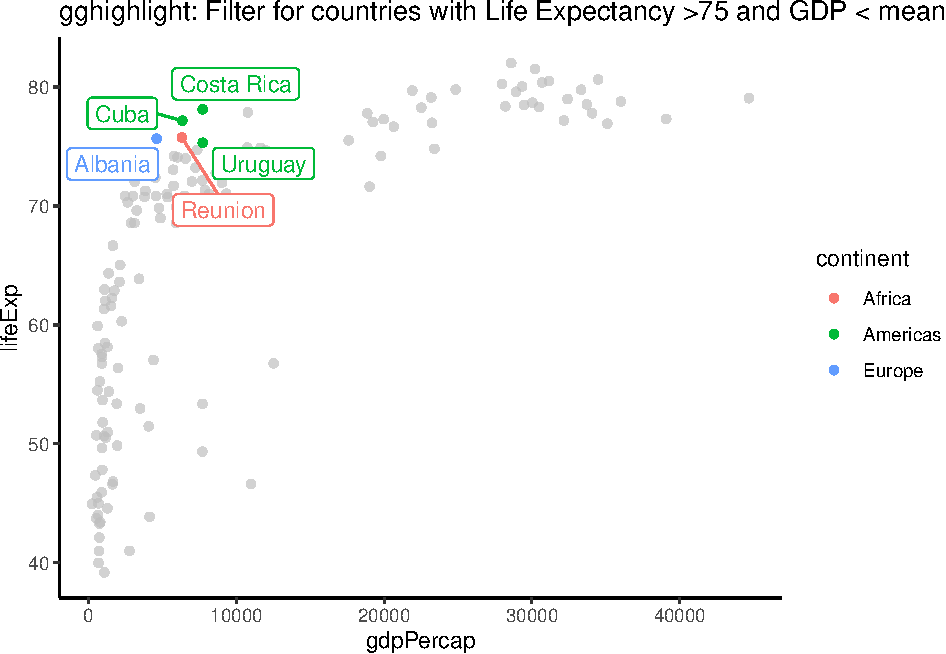
\includegraphics{06-plotting_files/figure-latex/gghighlight-1.pdf}

\hypertarget{coord_flip-factor-orders}{%
\section{\texorpdfstring{\texttt{coord\_flip()} factor orders}{coord\_flip() factor orders}}\label{coord_flip-factor-orders}}

\begin{Shaded}
\begin{Highlighting}[]
\FunctionTok{library}\NormalTok{(ggplot2)}

\CommentTok{\# unflipped (yes this plot has no purpose :)}
\NormalTok{gapminder }\SpecialCharTok{\%\textgreater{}\%} 
  \FunctionTok{ggplot}\NormalTok{(}\FunctionTok{aes}\NormalTok{(}\AttributeTok{x =}\NormalTok{ continent, }\AttributeTok{fill =} \FunctionTok{factor}\NormalTok{(year))) }\SpecialCharTok{+} 
  \FunctionTok{geom\_bar}\NormalTok{() }\SpecialCharTok{+} 
  \FunctionTok{scale\_fill\_brewer}\NormalTok{(}\AttributeTok{palette =} \StringTok{"Paired"}\NormalTok{)}
\end{Highlighting}
\end{Shaded}

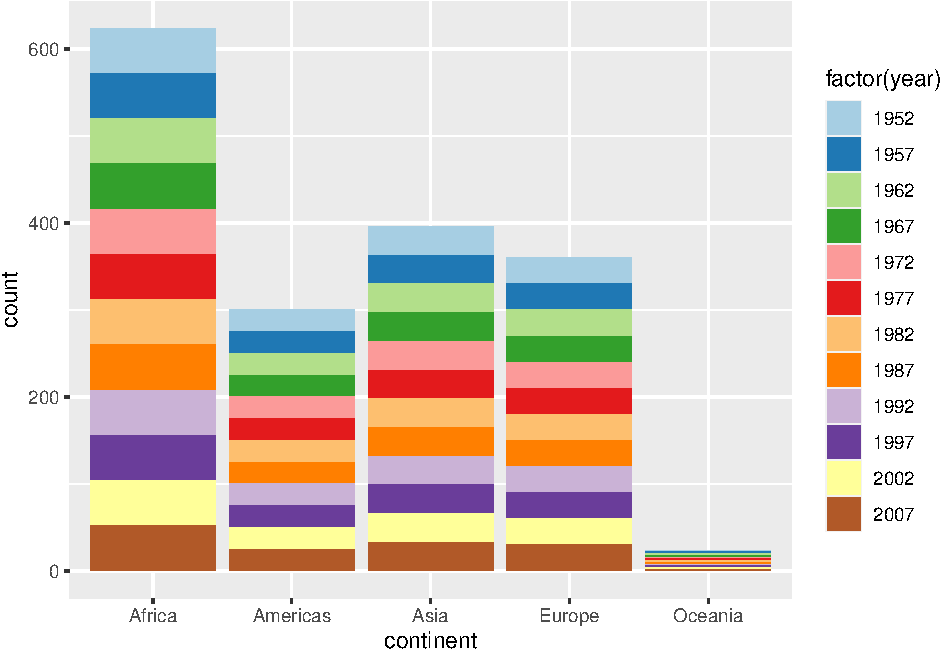
\includegraphics{06-plotting_files/figure-latex/unnamed-chunk-1-1.pdf}

\begin{Shaded}
\begin{Highlighting}[]
\CommentTok{\# flipped}
\NormalTok{gapminder }\SpecialCharTok{\%\textgreater{}\%} 
  \FunctionTok{ggplot}\NormalTok{(}\FunctionTok{aes}\NormalTok{(}\AttributeTok{x =} \FunctionTok{fct\_rev}\NormalTok{(continent), }\AttributeTok{fill =} \FunctionTok{factor}\NormalTok{(year))) }\SpecialCharTok{+} 
  \FunctionTok{geom\_bar}\NormalTok{() }\SpecialCharTok{+} 
  \FunctionTok{coord\_flip}\NormalTok{() }\SpecialCharTok{+} 
  \FunctionTok{scale\_fill\_brewer}\NormalTok{(}\AttributeTok{palette =} \StringTok{"Paired"}\NormalTok{, }\AttributeTok{breaks =}\NormalTok{ rev) }\SpecialCharTok{+} 
  \FunctionTok{guides}\NormalTok{(}\AttributeTok{fill =} \FunctionTok{guide\_legend}\NormalTok{(}\AttributeTok{reverse =} \ConstantTok{TRUE}\NormalTok{))}
\end{Highlighting}
\end{Shaded}

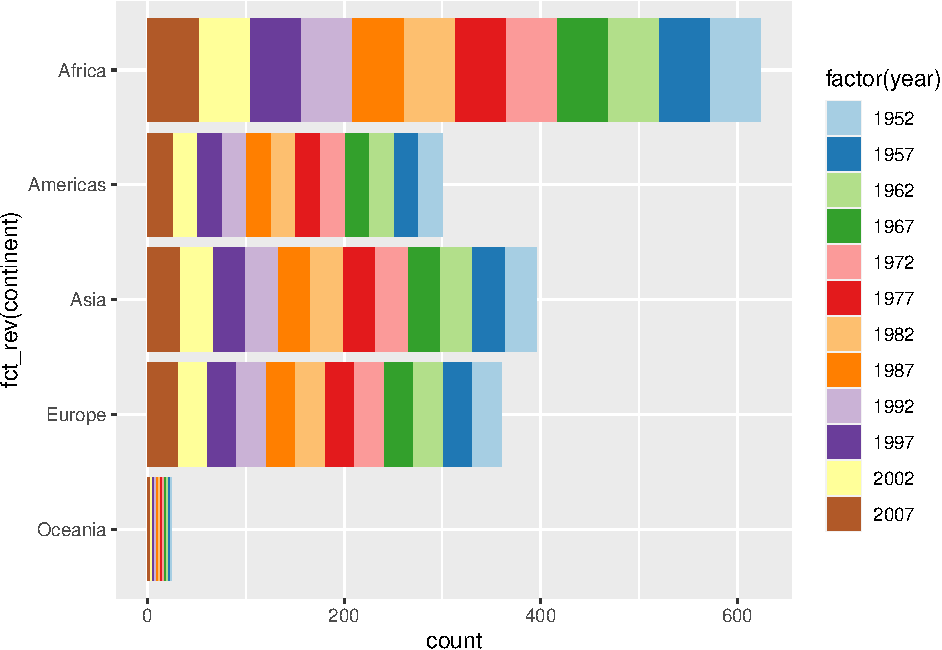
\includegraphics{06-plotting_files/figure-latex/unnamed-chunk-1-2.pdf}

\begin{Shaded}
\begin{Highlighting}[]
\DocumentationTok{\#\# This is actually the same as the previous plot so is achieving the aim. }
\DocumentationTok{\#\# But the unflipped plot isn\textquotesingle{}t that great given the order of the year}
\DocumentationTok{\#\# Hence why wanting to flip}

\CommentTok{\# Better flipped}
\CommentTok{\# This way, new fill levels get added on the end}
\NormalTok{gapminder }\SpecialCharTok{\%\textgreater{}\%} 
  \FunctionTok{ggplot}\NormalTok{(}\FunctionTok{aes}\NormalTok{(}\AttributeTok{x =} \FunctionTok{fct\_rev}\NormalTok{(continent), }\AttributeTok{fill =} \FunctionTok{fct\_rev}\NormalTok{(}\FunctionTok{factor}\NormalTok{(year)))) }\SpecialCharTok{+} 
  \FunctionTok{geom\_bar}\NormalTok{() }\SpecialCharTok{+} 
  \FunctionTok{coord\_flip}\NormalTok{() }\SpecialCharTok{+} 
  \FunctionTok{scale\_fill\_brewer}\NormalTok{(}\AttributeTok{palette =} \StringTok{"Paired"}\NormalTok{, }\AttributeTok{breaks =}\NormalTok{ rev, }\AttributeTok{direction =} \SpecialCharTok{{-}}\DecValTok{1}\NormalTok{)}
\end{Highlighting}
\end{Shaded}

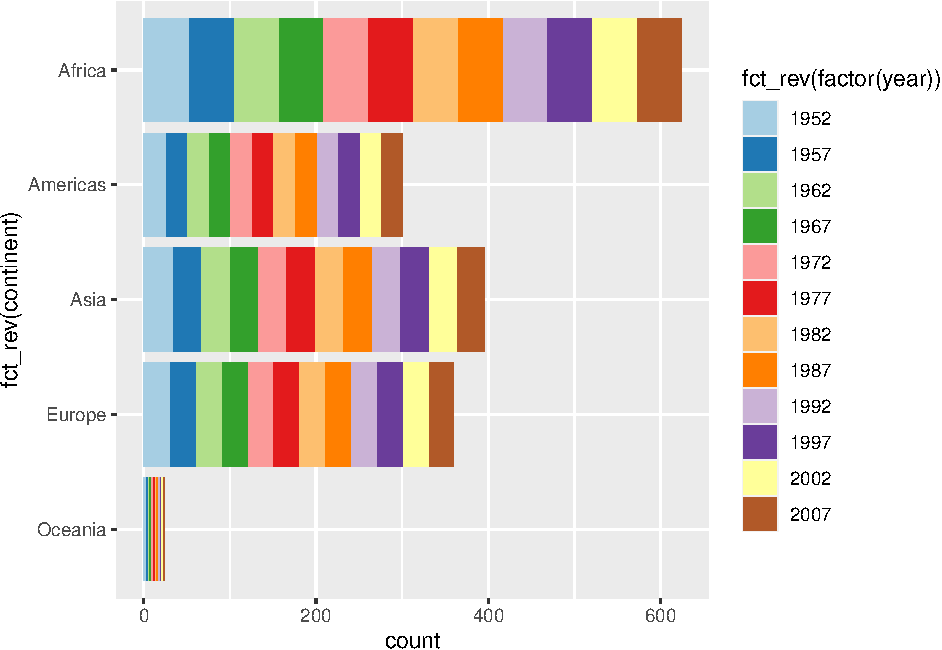
\includegraphics{06-plotting_files/figure-latex/unnamed-chunk-1-3.pdf}

\hypertarget{axis-font-size}{%
\section{Axis font size}\label{axis-font-size}}

\begin{Shaded}
\begin{Highlighting}[]
\CommentTok{\# OPTION 1: theme(axis.text = element\_text(size = 12, colour = "black"))}
\CommentTok{\# OPTION 2: width and height arguments of ggsave()}

\FunctionTok{library}\NormalTok{(tidyverse)}
\FunctionTok{library}\NormalTok{(scales)}

\CommentTok{\# made{-}up example data}
\NormalTok{mydata }\OtherTok{=} \FunctionTok{tibble}\NormalTok{(}\AttributeTok{group    =} \FunctionTok{c}\NormalTok{(}\StringTok{"UMIC"}\NormalTok{, }\StringTok{"LMIC"}\NormalTok{, }\StringTok{"LIC"}\NormalTok{) }\SpecialCharTok{\%\textgreater{}\%} \FunctionTok{rep}\NormalTok{(}\AttributeTok{each =} \DecValTok{2}\NormalTok{),}
                \AttributeTok{value    =} \DecValTok{1}\SpecialCharTok{:}\DecValTok{6}\NormalTok{, }
                \AttributeTok{variable =} \FunctionTok{c}\NormalTok{(}\StringTok{"Yes"}\NormalTok{, }\StringTok{"No"}\NormalTok{) }\SpecialCharTok{\%\textgreater{}\%} \FunctionTok{rep}\NormalTok{(}\DecValTok{3}\NormalTok{))}

\NormalTok{mydata }\SpecialCharTok{\%\textgreater{}\%} 
  \FunctionTok{ggplot}\NormalTok{(}\FunctionTok{aes}\NormalTok{(}\AttributeTok{x =}\NormalTok{ group, }\AttributeTok{y =}\NormalTok{ value, }\AttributeTok{fill =}\NormalTok{ variable)) }\SpecialCharTok{+}
  \FunctionTok{geom\_col}\NormalTok{(}\AttributeTok{position =} \StringTok{"fill"}\NormalTok{) }\SpecialCharTok{+}
  \FunctionTok{scale\_y\_continuous}\NormalTok{(}\AttributeTok{labels =}\NormalTok{ percent, }\AttributeTok{expand =} \FunctionTok{c}\NormalTok{(}\DecValTok{0}\NormalTok{, }\DecValTok{0}\NormalTok{)) }\SpecialCharTok{+}
  \FunctionTok{theme\_bw}\NormalTok{() }\SpecialCharTok{+}
  \CommentTok{\# OPTION 1: change font with theme()}
  \FunctionTok{theme}\NormalTok{(}\AttributeTok{axis.text  =} \FunctionTok{element\_text}\NormalTok{(}\AttributeTok{size =} \DecValTok{12}\NormalTok{, }\AttributeTok{colour =} \StringTok{"black"}\NormalTok{),}
        \AttributeTok{axis.title =} \FunctionTok{element\_blank}\NormalTok{())}
\end{Highlighting}
\end{Shaded}

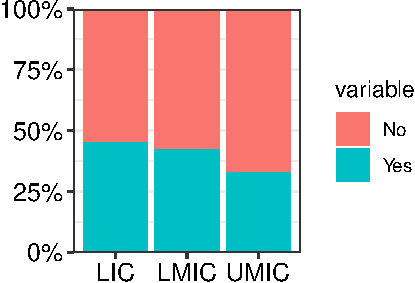
\includegraphics{06-plotting_files/figure-latex/unnamed-chunk-2-1.pdf}

\begin{Shaded}
\begin{Highlighting}[]
\CommentTok{\# OPTION 2: play around with export size. Since PDF will always have max resolution anyway}
\CommentTok{\# but changing width and height modifies text size}
\NormalTok{mywidth  }\OtherTok{=} \DecValTok{5}
\NormalTok{myheight }\OtherTok{=} \DecValTok{4}
\CommentTok{\#ggsave("barplot\_5x4.pdf", width = mywidth, height = myheight)}

\NormalTok{mywidth  }\OtherTok{=} \DecValTok{10}
\NormalTok{myheight }\OtherTok{=} \DecValTok{8}
\CommentTok{\#ggsave("barplot\_10x8.pdf", width = mywidth, height = myheight)}
\end{Highlighting}
\end{Shaded}

Same plot 5x4 inches vs 10x8 inches:

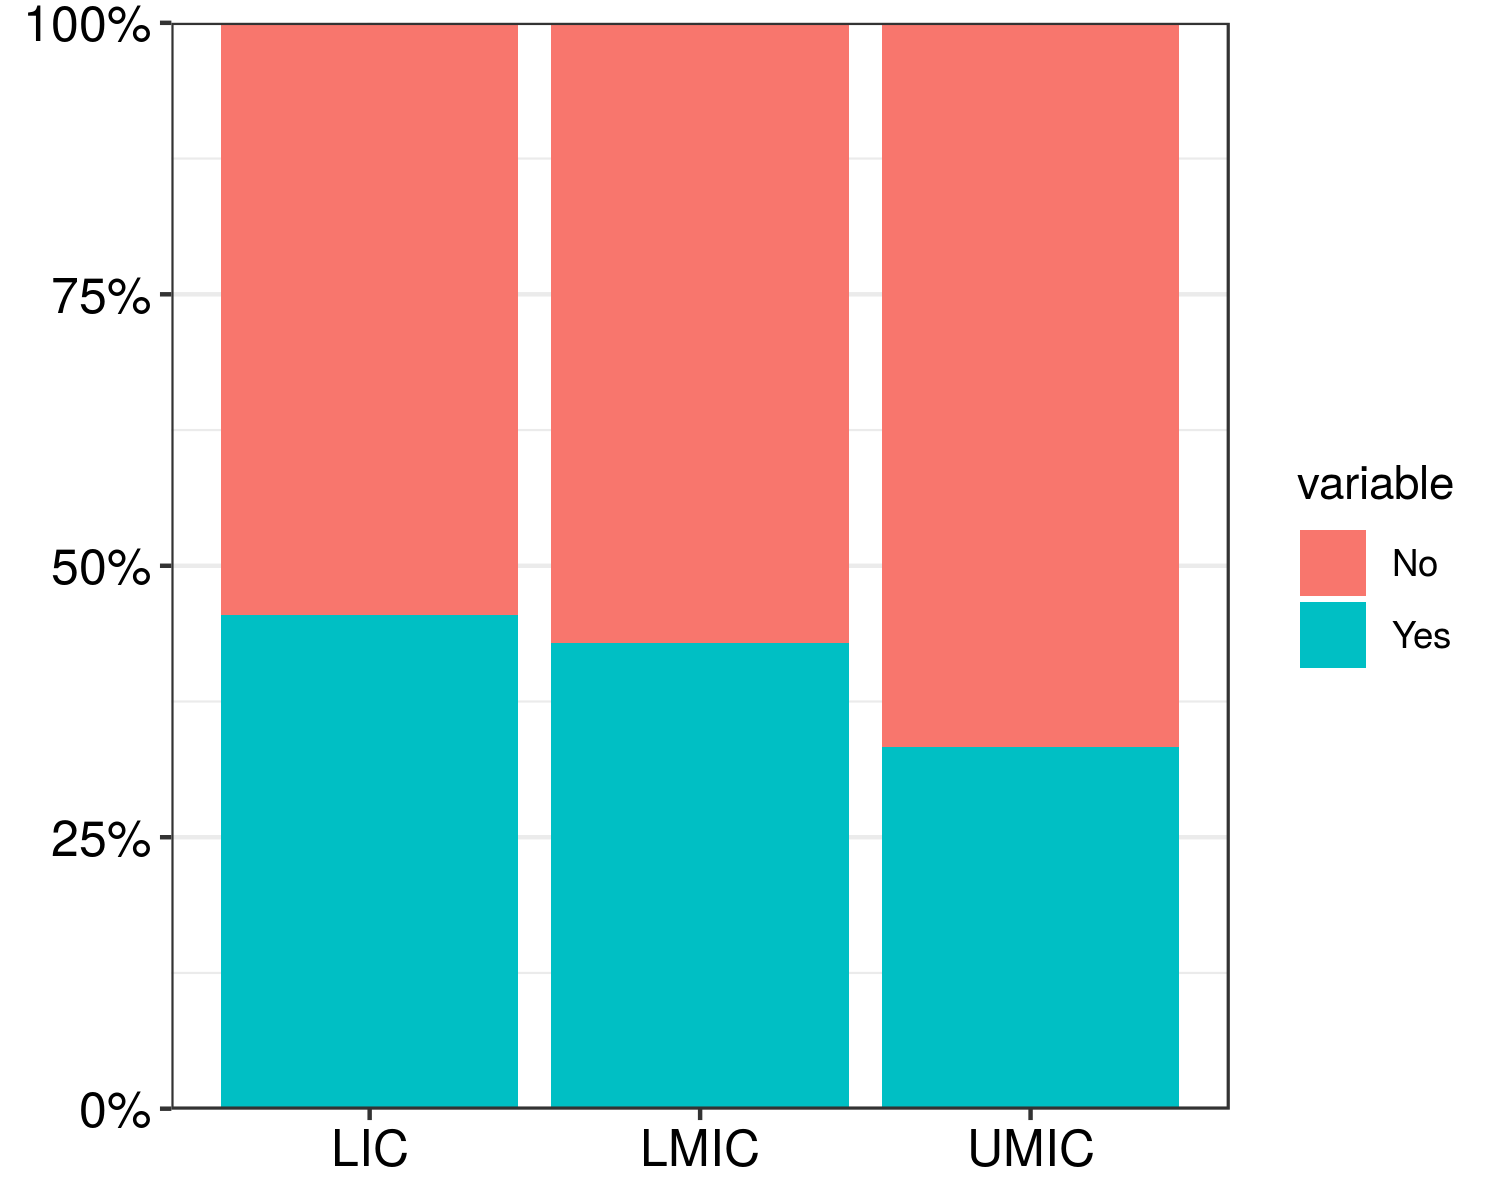
\includegraphics[width=0.5\linewidth]{img/barplot_5x4}
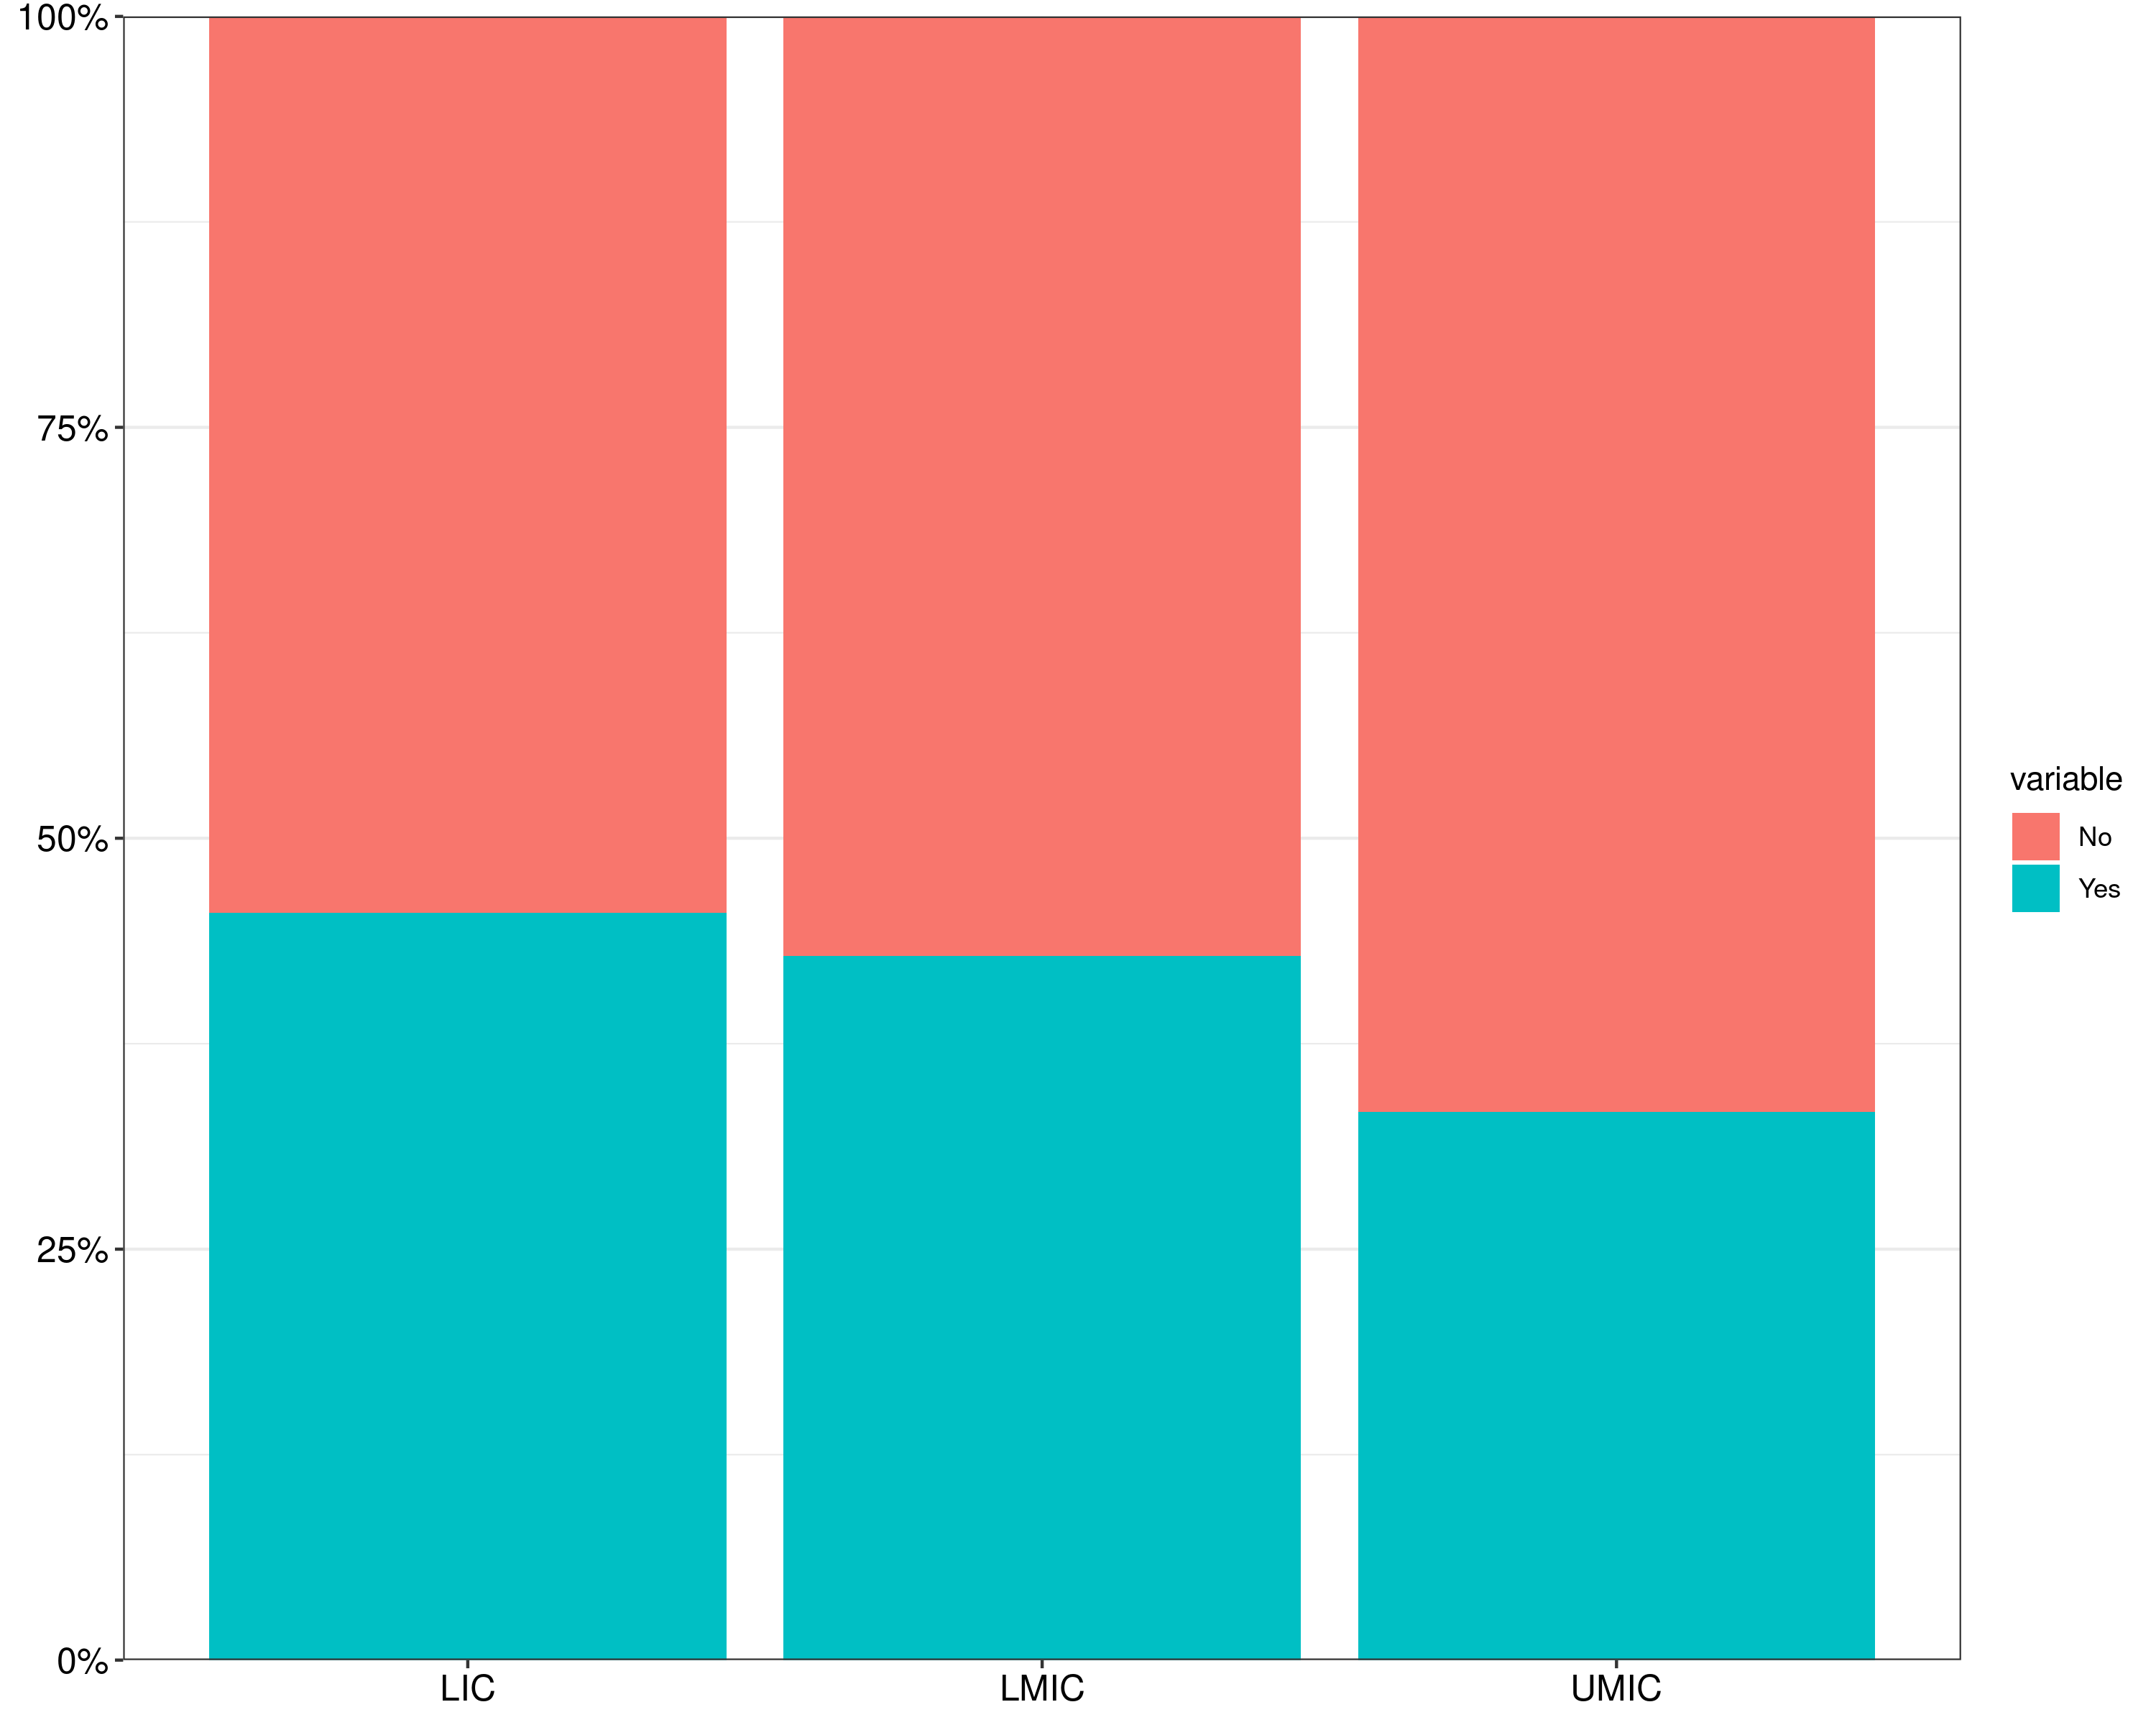
\includegraphics[width=0.5\linewidth]{img/barplot_10x8}

\hypertarget{shorten-arrows-on-a-dag}{%
\section{Shorten Arrows on a DAG}\label{shorten-arrows-on-a-dag}}

Plot 1 with large nodes and arrows not shortened:

\begin{Shaded}
\begin{Highlighting}[]
\NormalTok{DAG }\OtherTok{\textless{}{-}}\NormalTok{ ggdag}\SpecialCharTok{::}\FunctionTok{dagify}\NormalTok{(y }\SpecialCharTok{\textasciitilde{}}\NormalTok{ x)}
\NormalTok{DAG }\OtherTok{\textless{}{-}}\NormalTok{ ggdag}\SpecialCharTok{::}\FunctionTok{tidy\_dagitty}\NormalTok{(DAG)}
\NormalTok{PLOT1 }\OtherTok{\textless{}{-}}\NormalTok{ ggdag}\SpecialCharTok{::}\FunctionTok{ggdag}\NormalTok{(DAG, }\AttributeTok{node\_size =} \DecValTok{50}\NormalTok{)}
\NormalTok{PLOT1}
\end{Highlighting}
\end{Shaded}

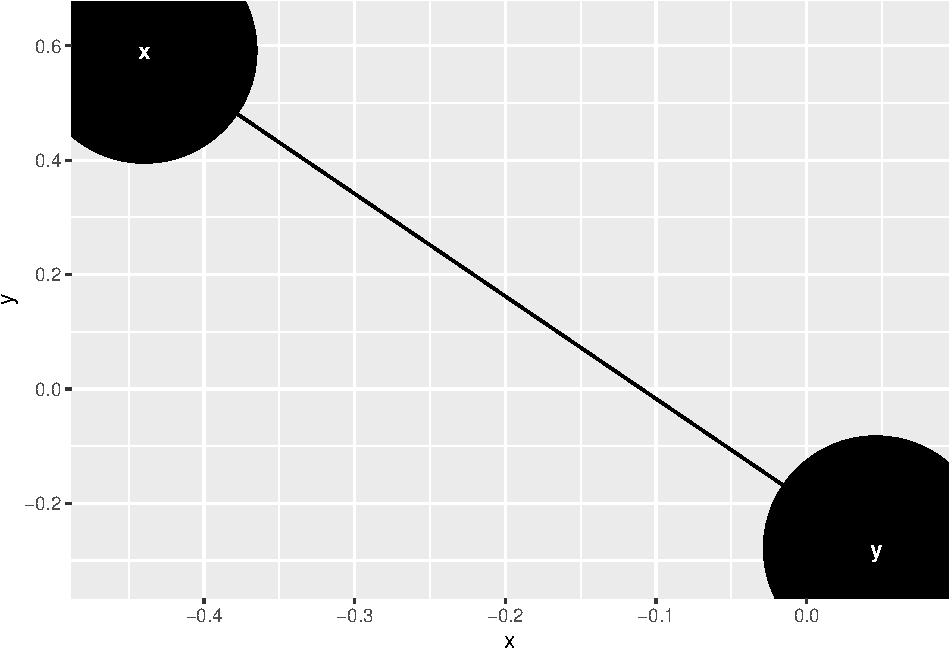
\includegraphics{06-plotting_files/figure-latex/dag_big_nodes_part_1-1.pdf}

\begin{Shaded}
\begin{Highlighting}[]
\NormalTok{shorten\_dag\_arrows }\OtherTok{\textless{}{-}} \ControlFlowTok{function}\NormalTok{(tidy\_dag, shorten\_distance)\{}
  \CommentTok{\# Update underlying ggdag object}
\NormalTok{  tidy\_dag}\SpecialCharTok{$}\NormalTok{data }\OtherTok{=}\NormalTok{ dplyr}\SpecialCharTok{::}\FunctionTok{mutate}\NormalTok{(tidy\_dag}\SpecialCharTok{$}\NormalTok{data, }\AttributeTok{slope =}\NormalTok{ (yend }\SpecialCharTok{{-}}\NormalTok{ y) }\SpecialCharTok{/}\NormalTok{ (xend }\SpecialCharTok{{-}}\NormalTok{ x), }\CommentTok{\# Calculate slope of line}
                  \AttributeTok{distance =} \FunctionTok{sqrt}\NormalTok{((xend}\SpecialCharTok{{-}}\NormalTok{x)}\SpecialCharTok{\^{}}\DecValTok{2} \SpecialCharTok{+}\NormalTok{ (yend }\SpecialCharTok{{-}}\NormalTok{ y)}\SpecialCharTok{\^{}}\DecValTok{2}\NormalTok{), }\CommentTok{\# Calculate total distance of line}
                  \AttributeTok{proportion =}\NormalTok{ shorten\_distance}\SpecialCharTok{/}\NormalTok{distance, }\CommentTok{\# Calculate proportion by which to be shortened}
                  \AttributeTok{xend =}\NormalTok{ (}\DecValTok{1}\SpecialCharTok{{-}}\NormalTok{proportion)}\SpecialCharTok{*}\NormalTok{xend }\SpecialCharTok{+}\NormalTok{ (proportion}\SpecialCharTok{*}\NormalTok{x), }\CommentTok{\# Shorten xend}
                  \AttributeTok{yend =}\NormalTok{ (}\DecValTok{1}\SpecialCharTok{{-}}\NormalTok{proportion)}\SpecialCharTok{*}\NormalTok{yend }\SpecialCharTok{+}\NormalTok{ (proportion}\SpecialCharTok{*}\NormalTok{y)) }\SpecialCharTok{\%\textgreater{}\%} \CommentTok{\# Shorten yend}
\NormalTok{    dplyr}\SpecialCharTok{::}\FunctionTok{select}\NormalTok{(}\SpecialCharTok{{-}}\NormalTok{slope, }\SpecialCharTok{{-}}\NormalTok{distance, }\SpecialCharTok{{-}}\NormalTok{proportion) }\CommentTok{\# Drop intermediate values}
  \FunctionTok{return}\NormalTok{(tidy\_dag)}
\NormalTok{\}}
\NormalTok{DAG }\OtherTok{\textless{}{-}} \FunctionTok{shorten\_dag\_arrows}\NormalTok{(DAG, }\AttributeTok{shorten\_distance =} \FloatTok{0.1}\NormalTok{)}
\NormalTok{PLOT2 }\OtherTok{\textless{}{-}}\NormalTok{ ggdag}\SpecialCharTok{::}\FunctionTok{ggdag}\NormalTok{(DAG, }\AttributeTok{node\_size =} \DecValTok{50}\NormalTok{)}
\NormalTok{PLOT2}
\end{Highlighting}
\end{Shaded}

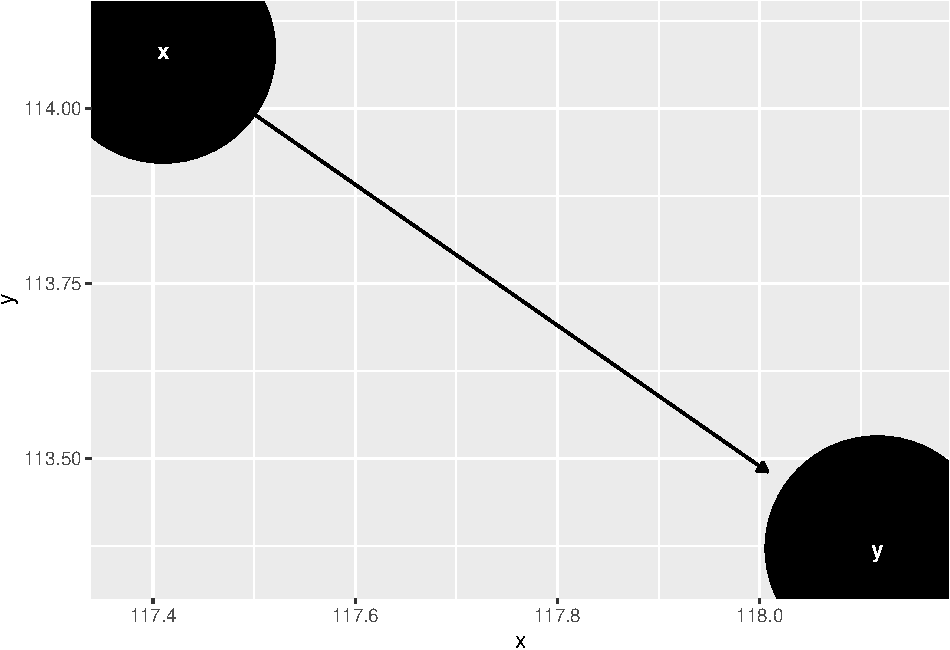
\includegraphics{06-plotting_files/figure-latex/dag_big_nodes_part_2-1.pdf}

\hypertarget{genomics}{%
\chapter{Genomics}\label{genomics}}

\hypertarget{single-cell-analysis}{%
\section{Single Cell Analysis}\label{single-cell-analysis}}

\hypertarget{minimising-the-size-of-a-seurat-object}{%
\subsection{Minimising the size of a Seurat Object}\label{minimising-the-size-of-a-seurat-object}}

Single cell analyses are ofetn collated in Seurat objects which can be huge. We reduced the size of our Seurat object by pulling the relevant sections using the code below reducing the object to \textless20\% of its original size. This works by only including the sparse matrices. This is not a workable example, but the PBMC dataset could be used if necessary.

\begin{Shaded}
\begin{Highlighting}[]
\CommentTok{\#library(Seurat)}
\CommentTok{\#library(dplyr)}


\CommentTok{\#Load in the data}

\NormalTok{pathtoglobaldata }\OtherTok{\textless{}{-}}\StringTok{"mac\_shiny/data/Global\_sc\_object"}
\NormalTok{object\_global}\OtherTok{\textless{}{-}}\FunctionTok{readRDS}\NormalTok{(pathtoglobaldata)}


\CommentTok{\# Get sparse assay data}
\NormalTok{sizetest\_global}\OtherTok{\textless{}{-}}\FunctionTok{GetAssayData}\NormalTok{(}\AttributeTok{object =}\NormalTok{ object\_global, }\AttributeTok{slot =} \StringTok{"data"}\NormalTok{) }\CommentTok{\# counts don’t work, scaled breaks my pc with memory errors, not sure it matters that much}
\NormalTok{object\_global\_small}\OtherTok{\textless{}{-}} \FunctionTok{CreateSeuratObject}\NormalTok{(sizetest\_global)}

\CommentTok{\# Add in classifications. }

\NormalTok{object\_global\_small}\SpecialCharTok{@}\NormalTok{reductions}\SpecialCharTok{$}\NormalTok{tsne}\OtherTok{\textless{}{-}}\NormalTok{object\_global}\SpecialCharTok{@}\NormalTok{reductions}\SpecialCharTok{$}\NormalTok{tsne }\CommentTok{\# reduction embeddings for tsnegraph}
\NormalTok{object\_global\_small}\SpecialCharTok{$}\NormalTok{Phenotype}\OtherTok{\textless{}{-}}\NormalTok{ object\_global}\SpecialCharTok{$}\NormalTok{Phenotype}

\NormalTok{object\_global\_small}\SpecialCharTok{@}\NormalTok{meta.data}\SpecialCharTok{$}\NormalTok{final\_classification}\OtherTok{\textless{}{-}}\NormalTok{ object\_global}\SpecialCharTok{@}\NormalTok{meta.data}\SpecialCharTok{$}\NormalTok{final\_classification}
\NormalTok{object\_global\_small}\SpecialCharTok{$}\NormalTok{final\_classificaiton}\OtherTok{\textless{}{-}}\NormalTok{ object\_global}\SpecialCharTok{$}\NormalTok{final\_classification }\CommentTok{\#cell classifications}
\FunctionTok{Idents}\NormalTok{(}\AttributeTok{object =}\NormalTok{ object\_global\_small) }\OtherTok{\textless{}{-}} \StringTok{"final\_classificaiton"} \CommentTok{\#set forever}


\CommentTok{\#same}
\FunctionTok{saveRDS}\NormalTok{(object\_global\_small,}\StringTok{"mac\_shiny/data/global\_object\_sml"}\NormalTok{)}
\end{Highlighting}
\end{Shaded}

\hypertarget{programming-in-rlang}{%
\chapter{Programming in rlang}\label{programming-in-rlang}}

\hypertarget{rlang}{%
\section{rlang}\label{rlang}}

\hypertarget{what-is-rlang}{%
\subsection{What is rlang?}\label{what-is-rlang}}

rlang is a low-level programming API for R which the tidyverse uses (meaning it speaks to R in as R like way as possible, rather than a `high-level' - high level is more user orientated and interpretable). It enables you to extend what the tidyverse can do and adapt it for your own uses. It's particularly good to use if you're doing lots of more `programming' type R work, for example, building a package, making a complex shiny app or writing functions. It might also be handy if you're doing lots of big data manipulation and want to manipulate different datasets in the same way, for example.

In this chapter we'll discuss some uses of it.

\hypertarget{dynamic-calling-of-variables-using-dplyr}{%
\subsection{Dynamic calling of variables using dplyr}\label{dynamic-calling-of-variables-using-dplyr}}

In this example, say we have a tibble of variables, but we want to apply dynamic changes to it (so we feed R a variable, that can change, either using another function like \texttt{purr::map} or in a ShinyApp). In this instance, specifying each variable and each different possible consequence using different logical functions would take forever and be very clunky. So we can use rlang to simply put a dynamic variable/object through the same function.

We'll use an example where we want to summarise by different outcomes in a dynamic way.

\begin{Shaded}
\begin{Highlighting}[]
\FunctionTok{library}\NormalTok{(tidyverse)}
\CommentTok{\#Make data {-} here nonsense numbers on deaths per 100k from guns say}

\NormalTok{example\_data }\OtherTok{=} \FunctionTok{tibble}\NormalTok{(}\AttributeTok{countries =} \FunctionTok{c}\NormalTok{(}\StringTok{\textquotesingle{}UK\textquotesingle{}}\NormalTok{, }\StringTok{\textquotesingle{}USA\textquotesingle{}}\NormalTok{, }\StringTok{\textquotesingle{}Pakistan\textquotesingle{}}\NormalTok{, }\StringTok{\textquotesingle{}Mexico\textquotesingle{}}\NormalTok{, }\StringTok{\textquotesingle{}Ireland\textquotesingle{}}\NormalTok{, }\StringTok{\textquotesingle{}Estonia\textquotesingle{}}\NormalTok{),}
                      \AttributeTok{region =} \FunctionTok{c}\NormalTok{(}\StringTok{\textquotesingle{}Europe\textquotesingle{}}\NormalTok{, }\StringTok{\textquotesingle{}Americas\textquotesingle{}}\NormalTok{, }\StringTok{\textquotesingle{}Asia\textquotesingle{}}\NormalTok{, }\StringTok{\textquotesingle{}Americas\textquotesingle{}}\NormalTok{, }\StringTok{\textquotesingle{}Europe\textquotesingle{}}\NormalTok{, }\StringTok{\textquotesingle{}Europe\textquotesingle{}}\NormalTok{),}
                      \AttributeTok{Death\_from\_guns =} \FunctionTok{c}\NormalTok{(}\DecValTok{1}\NormalTok{, }\DecValTok{200}\NormalTok{, }\DecValTok{150}\NormalTok{, }\DecValTok{450}\NormalTok{, }\DecValTok{3}\NormalTok{, }\FloatTok{3.5}\NormalTok{),}
                      \AttributeTok{Death\_from\_smoking =} \FunctionTok{c}\NormalTok{(}\DecValTok{100}\NormalTok{, }\DecValTok{300}\NormalTok{, }\DecValTok{140}\NormalTok{, }\DecValTok{150}\NormalTok{, }\DecValTok{120}\NormalTok{, }\DecValTok{300}\NormalTok{))}


\CommentTok{\#example function for summarising using dynamic variables and bang bangs}
\CommentTok{\#note metric must be numeric}
\NormalTok{summarise\_feature }\OtherTok{=} \ControlFlowTok{function}\NormalTok{(df, col\_var, ...)\{}
  \FunctionTok{require}\NormalTok{(tidyverse)}
  
\NormalTok{  wurly\_curly }\OtherTok{=} \ControlFlowTok{function}\NormalTok{(.)\{}\CommentTok{\#The wurly\_curly function makes things nicer}
  \FunctionTok{require}\NormalTok{(rlang)}
  \SpecialCharTok{!!}\FunctionTok{quo\_name}\NormalTok{(}\FunctionTok{enquo}\NormalTok{(.))\}}

\NormalTok{  summary\_nm\_sum }\OtherTok{\textless{}{-}} \FunctionTok{paste0}\NormalTok{(}\StringTok{"metric\_"}\NormalTok{, }\FunctionTok{wurly\_curly}\NormalTok{(col\_var))}\CommentTok{\#The new LHS variable must have a different name from that on the RHS}

\NormalTok{  df }\SpecialCharTok{\%\textgreater{}\%}
    \FunctionTok{group\_by}\NormalTok{(...) }\SpecialCharTok{\%\textgreater{}\%} 
    \FunctionTok{summarise}\NormalTok{(}\SpecialCharTok{!!}\AttributeTok{summary\_nm\_sum :=} \FunctionTok{sum}\NormalTok{(\{\{col\_var\}\}))}
\NormalTok{\}}


\CommentTok{\#output new variable}
\NormalTok{example\_data }\SpecialCharTok{\%\textgreater{}\%} 
  \FunctionTok{summarise\_feature}\NormalTok{(Death\_from\_guns, region) }

\CommentTok{\#How to dynamically change names using mutate and rlang}
\CommentTok{\#Bang bang variables into mutate/tidyverse(so they can be dynamically changed)}

\CommentTok{\#Select metric}
\NormalTok{metric }\OtherTok{=} \StringTok{\textquotesingle{}metric\_Death\_from\_guns\textquotesingle{}} \CommentTok{\#example but can be any named column}

\NormalTok{metric\_mutate }\OtherTok{=} \FunctionTok{paste0}\NormalTok{(}\StringTok{\textquotesingle{}prefix\_\textquotesingle{}}\NormalTok{, metric) }\CommentTok{\#some reason doesn\textquotesingle{}t take these within the mutate function so has to be outside}

\NormalTok{example\_data }\SpecialCharTok{\%\textgreater{}\%} 
  \FunctionTok{summarise\_feature}\NormalTok{(Death\_from\_guns, region) }\SpecialCharTok{\%\textgreater{}\%} 
  \FunctionTok{mutate}\NormalTok{(}\SpecialCharTok{!!}\AttributeTok{metric\_mutate :=} \SpecialCharTok{!!}\NormalTok{rlang}\SpecialCharTok{::}\FunctionTok{sym}\NormalTok{(metric) }\SpecialCharTok{*} \DecValTok{2}\NormalTok{)}\CommentTok{\#apply arbitary multiplication by two}
\end{Highlighting}
\end{Shaded}

\hypertarget{server-admin}{%
\chapter{Server admin}\label{server-admin}}

\hypertarget{rstudio-argonaut-and-argosafe}{%
\section{RStudio (argonaut and argosafe)}\label{rstudio-argonaut-and-argosafe}}

\hypertarget{scheduled-script-cron}{%
\subsection{Scheduled script (CRON)}\label{scheduled-script-cron}}

Most scheduling is best done using RStudio Connect (argoshare), see below.
For certain applications, it may be desirable to do this on argonaut or argosafe.
For instance, if a scheduled job is required to be done in a trusted research environment.

This can be done by adding a cron job.

The following will execute the \texttt{R} script at 7AM everyday. A log file is written within the project.

\begin{Shaded}
\begin{Highlighting}[]
\ExtensionTok{crontab} \AttributeTok{{-}e}

\CommentTok{\# Add line (using e.g. nano editor)}
\ExtensionTok{00}\NormalTok{ 07 }\PreprocessorTok{*} \PreprocessorTok{*} \PreprocessorTok{*}\NormalTok{ Rscript /home/user/project/script.R }\OperatorTok{\&\textgreater{}\textgreater{}}\NormalTok{ /home/user/project/cron.log}
\end{Highlighting}
\end{Shaded}

The cronjob does not load the user environment.
If you are using environment variables in R, e.g.~API tokens, then these can be loaded within the R script.
Include this at the top of your script.

\begin{Shaded}
\begin{Highlighting}[]
\CommentTok{\# Log}
\FunctionTok{print}\NormalTok{(}\FunctionTok{paste}\NormalTok{(}\StringTok{"Start:"}\NormalTok{, }\FunctionTok{Sys.time}\NormalTok{()))}

\CommentTok{\# Environment variables}
\FunctionTok{readRenviron}\NormalTok{(}\StringTok{"/home/user/.Renviron"}\NormalTok{)}
\end{Highlighting}
\end{Shaded}

\hypertarget{rstudio-connect-argoshare}{%
\section{RStudio Connect: argoshare}\label{rstudio-connect-argoshare}}

\hypertarget{delete-user}{%
\subsection{Delete user}\label{delete-user}}

\begin{Shaded}
\begin{Highlighting}[]
\CommentTok{\# Delete user from argoshare}
\CommentTok{\#\# Connect must be stopped first}
\FunctionTok{sudo}\NormalTok{ systemctl stop rstudio{-}connect}

\CommentTok{\#\# List all users}
\FunctionTok{sudo}\NormalTok{ /opt/rstudio{-}connect/bin/usermanager list}

\CommentTok{\#\# Find guid for the user you want to delete, looks like below. }
\CommentTok{\#\# Delete user {-} need to say y/n}
\FunctionTok{sudo}\NormalTok{ /opt/rstudio{-}connect/bin/usermanager delete }\AttributeTok{{-}{-}users} \AttributeTok{{-}{-}user{-}guid}\NormalTok{ 46cb5adb{-}4036{-}451f{-}9f08{-}0da3197dbc6c}

\CommentTok{\#\# Restart connect}
\FunctionTok{sudo}\NormalTok{ systemctl start rstudio{-}connect}
\end{Highlighting}
\end{Shaded}

\hypertarget{shiny-server-opensource-setup---uoe-eleanor}{%
\section{Shiny server opensource setup - UoE Eleanor}\label{shiny-server-opensource-setup---uoe-eleanor}}

This guide assumes you're already on the University of Edinburgh local network. If you're working from home, you'll first need to connect the UoE VPN. It also assumes you already have storage allocated to your project on Eleanor, and that your own computer is either Linux-based or a Mac.

\hypertarget{setting-up-ubuntu-instance}{%
\subsection{Setting up Ubuntu Instance}\label{setting-up-ubuntu-instance}}

\begin{itemize}
\tightlist
\item
  Log into the Openstack dashboard on Horizon - \url{https://horizon.ecdf.ed.ac.uk/dashboard/}
\item
  Click on Instances and launch a new instance (Ubuntu 18.4, t1.small (free tier))
\item
  Click on key pairs and create an SSH keypair, for securely logging on to the new instance.
\item
  Save the private key to a secure place on your computer (\textasciitilde/.ssh is the usual spot for these things). Change the files permissions to make it secure. Eleanor will not let you SSH without this step. In a local terminal, type:
\end{itemize}

\begin{Shaded}
\begin{Highlighting}[]
\FunctionTok{chmod}\NormalTok{ 400 PATH{-}TO{-}PRIVATE{-}KEY}
\end{Highlighting}
\end{Shaded}

\begin{itemize}
\tightlist
\item
  Click on Network \textgreater{} Floating IPs and create a new floating IP. Associate it with your new instance. Make a note of your floating IP -- this is the address you'll use to access your instance from now on.
\item
  Click on Security Groups and create a new security group. Add new rules to this group, allowing TCP ingress and egress on the following ports: 80 (HTTP), 22 (SSH), 3838 (Shiny Server).
\item
  Log into your instance using SSH. In a local terminal type:
\end{itemize}

\begin{Shaded}
\begin{Highlighting}[]
\FunctionTok{ssh} \AttributeTok{{-}i}\NormalTok{ PATH{-}TO{-}PRIVATE{-}KEY ubuntu@YOUR{-}FLOATING{-}IP}

\CommentTok{\#All being well, you’ll now have a terminal for your lovely new Ububtu instance.}
\CommentTok{\#Get your instance up{-}to{-}date. Run:}

\FunctionTok{sudo}\NormalTok{ apt{-}get update }\KeywordTok{\&\&} \FunctionTok{sudo}\NormalTok{ apt{-}get upgrade}
\end{Highlighting}
\end{Shaded}

\hypertarget{install-nginx}{%
\subsection{Install Nginx}\label{install-nginx}}

Nginx is the fast and light webserver that will host you Shiny code.

\begin{Shaded}
\begin{Highlighting}[]

\CommentTok{\#Install nginx}
\FunctionTok{sudo}\NormalTok{ apt{-}get }\AttributeTok{{-}y}\NormalTok{ install nginx}
\end{Highlighting}
\end{Shaded}

\begin{itemize}
\tightlist
\item
  In a browser, enter your floating IP address. All being well, you should now get a ``Welcome to Nginx'' page.
\end{itemize}

\hypertarget{installing-r}{%
\subsection{Installing R}\label{installing-r}}

Installing the latest version of R isn't as easy as apt-get R. Sources and keys need to be added to the source.list file, then R can be installed (the latest version). The first command sets the sources to the RStudio mirror, then grabs keys to authenticate the installation. Enter the following commands in order:

\begin{Shaded}
\begin{Highlighting}[]

\FunctionTok{sudo}\NormalTok{ sh }\AttributeTok{{-}c} \StringTok{\textquotesingle{}echo "deb http://cran.rstudio.com/bin/linux/ubuntu bionic{-}cran35/" \textgreater{}\textgreater{} /etc/apt/sources.list\textquotesingle{}}
\FunctionTok{sudo}\NormalTok{ apt{-}key adv }\AttributeTok{{-}{-}keyserver}\NormalTok{ keyserver.ubuntu.com }\AttributeTok{{-}{-}recv{-}keys}\NormalTok{ E298A3A825C0D65DFD57CBB651716619E084DAB9}

\FunctionTok{sudo}\NormalTok{ apt{-}get update}
\FunctionTok{sudo}\NormalTok{ apt{-}get }\AttributeTok{{-}y}\NormalTok{ install r{-}base}


\CommentTok{\#Now load R}
\ExtensionTok{R}
\CommentTok{\#Enter the following in the R console}
\FunctionTok{sessionInfo()}
\FunctionTok{quit()}
\end{Highlighting}
\end{Shaded}

\hypertarget{installing-shiny-server}{%
\subsection{Installing Shiny Server}\label{installing-shiny-server}}

There are a few external libraries that are required to use Shiny Server. Let's install those, the R package shiny then move on to installing Shiny Server itself.

\begin{Shaded}
\begin{Highlighting}[]

\FunctionTok{sudo}\NormalTok{ apt{-}get }\AttributeTok{{-}y}\NormalTok{ install gdebi{-}core}
\FunctionTok{sudo}\NormalTok{ su }\AttributeTok{{-}} \AttributeTok{{-}c} \StringTok{"R {-}e }\DataTypeTok{\textbackslash{}"}\StringTok{install.packages(\textquotesingle{}shiny\textquotesingle{}, repos=\textquotesingle{}http://cran.rstudio.com/\textquotesingle{})}\DataTypeTok{\textbackslash{}"}\StringTok{"}
\FunctionTok{wget}\NormalTok{ https://download3.rstudio.org/ubuntu{-}14.04/x86\_64/shiny{-}server{-}1.5.13.944{-}amd64.deb}
\FunctionTok{sudo}\NormalTok{ gdebi shiny{-}server{-}1.5.13.944{-}amd64.deb}
\end{Highlighting}
\end{Shaded}

Back in your browser, go to: YOUR-FLOATING-IP:3838
All being well, you'll get a Shiny Server test page.

\hypertarget{installing-other-linux-packages}{%
\subsection{Installing other Linux packages}\label{installing-other-linux-packages}}

You've got base-R installed and running now, but it's likely your Shiny app will have other unmet dependencies. Here are a few common packages you'll probably need, and the command needed to install them. Depending on your app, there may be others.

\begin{Shaded}
\begin{Highlighting}[]

\FunctionTok{sudo}\NormalTok{ apt{-}get install }\AttributeTok{{-}y} \DataTypeTok{\textbackslash{}}
\NormalTok{    pandoc }\DataTypeTok{\textbackslash{}}
\NormalTok{    pandoc{-}citeproc }\DataTypeTok{\textbackslash{}}
\NormalTok{    libssl{-}dev }\DataTypeTok{\textbackslash{}}
\NormalTok{    libcurl4{-}gnutls{-}dev }\DataTypeTok{\textbackslash{}}
\NormalTok{    libcairo2{-}dev }\DataTypeTok{\textbackslash{}}
\NormalTok{    libgdal{-}dev }\DataTypeTok{\textbackslash{}}
\NormalTok{    libgeos{-}dev }\DataTypeTok{\textbackslash{}}
\NormalTok{    libproj{-}dev }\DataTypeTok{\textbackslash{}}
\NormalTok{    libxml2{-}dev }\DataTypeTok{\textbackslash{}}
\NormalTok{    libxt{-}dev }\DataTypeTok{\textbackslash{}}
\NormalTok{    libv8{-}dev }\DataTypeTok{\textbackslash{}}
\NormalTok{    git}
\end{Highlighting}
\end{Shaded}

\hypertarget{installing-r-packages}{%
\subsection{Installing R packages}\label{installing-r-packages}}

You'll probably also need a bunch of extra libraries in R (we've already installed Shiny, but that's it). You install these from within R, rather than via apt-get. This is the syntax for installing R packages on the server -- just replace the package names with the ones your app requires.

\begin{Shaded}
\begin{Highlighting}[]

\FunctionTok{sudo}\NormalTok{ su }\AttributeTok{{-}} \AttributeTok{{-}c} \StringTok{"R {-}e }\DataTypeTok{\textbackslash{}"}\StringTok{install.packages(c(\textquotesingle{}rmarkdown\textquotesingle{}, \textquotesingle{}ggplot2\textquotesingle{}, \textquotesingle{}dplyr\textquotesingle{}, \textquotesingle{}sp\textquotesingle{}, \textquotesingle{}rgdal\textquotesingle{}, \textquotesingle{}rgeos\textquotesingle{}), repos=\textquotesingle{}http://cran.rstudio.com/\textquotesingle{})}\DataTypeTok{\textbackslash{}"}\StringTok{"}
\end{Highlighting}
\end{Shaded}

NB: Installing R packages can take a long time. As we're only using the small, free instance in this guide, you may find it grinds to a halt completely when trying to compile large libraries like seurat. This probably means you've run out of system memory. If that happens - see Setting up a swap file at the end of this guide.

\hypertarget{loading-your-app}{%
\subsection{Loading your app}\label{loading-your-app}}

Assuming you've developed your app on a local R-Studio server, getting it onto its new home can be surprisingly tricky. I've found by far the easiest way is to use an SFTP client, such as Cyberduck, giving it the username and key pair you've already set up and just sending the files straight into your home directory.

Once you've transferred them, you'll need to move them, including subdirectories, into /srv/shiny-server/.
Again, in your browser, go to YOUR-FLOATING-IP:3838. You'll either see your working app, or an error page listing missing dependencies. If it's the latter, follow the instructions above for installing R packages.

If you're not getting any useful error messages on the site, check out the app-specific log files in /var/log/shiny-server/

\hypertarget{make-your-app-the-default-index-page}{%
\subsection{Make your app the default index page}\label{make-your-app-the-default-index-page}}

You probably don't want visitors to your site to specify that they want port 3838, so now we're going to tell nginx to send visitors directly to your app.
First, we're going to edit the nginx config file.

\begin{Shaded}
\begin{Highlighting}[]
\FunctionTok{sudo}\NormalTok{ nano /etc/nginx/sites{-}available/default}

\CommentTok{\# Comment out (\#) any other active server config lines, and add this…}

\ExtensionTok{server}\NormalTok{ \{}
    \ExtensionTok{listen}\NormalTok{ 80}\KeywordTok{;}

    \ExtensionTok{location}\NormalTok{ / \{}
        \ExtensionTok{proxy\_pass}\NormalTok{ http://127.0.0.1:3838/}\KeywordTok{;}
        \ExtensionTok{proxy\_redirect}\NormalTok{ http://127.0.0.1:3838/ }\VariableTok{$scheme}\NormalTok{://}\VariableTok{$host}\NormalTok{/}\KeywordTok{;}
        \CommentTok{\# note, the following 3 lines added 2016{-}07{-}11, see updates section}
        \ExtensionTok{proxy\_http\_version}\NormalTok{ 1.1}\KeywordTok{;}
        \ExtensionTok{proxy\_set\_header}\NormalTok{ Upgrade }\VariableTok{$http\_upgrade}\KeywordTok{;}
        \ExtensionTok{proxy\_set\_header}\NormalTok{ Connection }\StringTok{"upgrade"}\KeywordTok{;}
     \ErrorTok{\}}
    \ErrorTok{\}}
\end{Highlighting}
\end{Shaded}

Next, we're going to update the Shiny server config file

\begin{Shaded}
\begin{Highlighting}[]

\FunctionTok{sudo}\NormalTok{ nano /etc/shiny{-}server/shiny{-}server.conf}

\CommentTok{\#Add the following (if it’s not already there, which it may well be):}

\ExtensionTok{server\{}
    \ExtensionTok{listen}\NormalTok{ 3838 127.0.0.1}\KeywordTok{;}

    \ExtensionTok{location}\NormalTok{ / \{}
      \ExtensionTok{site\_dir}\NormalTok{ /srv/shiny{-}server}\KeywordTok{;}
      \ExtensionTok{log\_dir}\NormalTok{ /var/log/shiny{-}server}\KeywordTok{;}
      \ExtensionTok{directory\_index}\NormalTok{ on}\KeywordTok{;}
    \ErrorTok{\}}
\ErrorTok{\}}
\end{Highlighting}
\end{Shaded}

Go to your floating IP in the browser, without the 3838, and all should be well.

\hypertarget{getting-a-user-friendly-domain-name}{%
\subsection{Getting a user-friendly domain name}\label{getting-a-user-friendly-domain-name}}

If you want to share your app with the outside world, you'll need to open it up beyond the UoE network and, preferably, give it a catchy URL.

Making your site public: Back in OpenStack, under the Network menu, click on Floating IP and disassociate your floating IP.
Now go up to Router and click clear gateway. Click Set Gateway and select Floating Network Public.
Back in Floating IPs, click Associate and select the external IP address (probably starting 129.x.x.x). Under port, select your instance.
Enter your external IP address into your browser, and your website should appear. It is now available outside the University network.

Setting up your domain name:
Your first step here is obviously to buy a domain name from one of the many providers on the internet.Once you have this, use your domain provider's dashboard to edit DNS settings. You're looking to change the ANAME or CNAME settings -- delete what's already there and set up a new ANAME record, with the public IP address of your site.

\hypertarget{appendix-1-password-protecting-your-site}{%
\subsection{Appendix 1 -- Password protecting your site}\label{appendix-1-password-protecting-your-site}}

You may want to add a basic password to your site. This is easily accomplished (though there are more robust password protection mechanisms out there, if you're dealing with potentially sensitive data).

First, make sure you have Apache2-utils installed:

\begin{Shaded}
\begin{Highlighting}[]
\CommentTok{\#First, make sure you have Apache2{-}utils installed:}
\FunctionTok{sudo}\NormalTok{ apt{-}get install apache2{-}utils}

\CommentTok{\#Now, stop nginx and shiny:}
\FunctionTok{sudo}\NormalTok{ service nginx stop}
\FunctionTok{sudo}\NormalTok{ stop shiny{-}server}

\CommentTok{\#Next, you’ll need to go back into that Nginx config file, with }
\FunctionTok{sudo}\NormalTok{ nano /etc/nginx/sites{-}available/default}

\CommentTok{\# Add the following two lines in the "location" section}
\ExtensionTok{location}\NormalTok{ / \{}
      \ExtensionTok{proxy\_pass}\NormalTok{ http://127.0.0.1:3838/}\KeywordTok{;}
      \ExtensionTok{proxy\_redirect}\NormalTok{ http://127.0.0.1:3838/ }\VariableTok{$scheme}\NormalTok{://}\VariableTok{$host}\NormalTok{/}\KeywordTok{;}
      \ExtensionTok{auth\_basic} \StringTok{"Username and Password are required"}\KeywordTok{;} 
      \ExtensionTok{auth\_basic\_user\_file}\NormalTok{ /etc/nginx/.htpasswd}\KeywordTok{;}
    \ErrorTok{\}}
\end{Highlighting}
\end{Shaded}

Once that's done, you'll need to edit Shiny Server's conf file so it only serves to loaclhost. Otherwise users would be able to creep around your authentication by going to port 3838.

\begin{Shaded}
\begin{Highlighting}[]
\FunctionTok{sudo}\NormalTok{ nano /etc/shiny{-}server/shiny{-}server.conf}

\CommentTok{\#Copy and paste the below to your shiny{-}server.conf.}
\ExtensionTok{server\{}
    \ExtensionTok{listen}\NormalTok{ 3838 127.0.0.1}\KeywordTok{;}
    
    \ExtensionTok{location}\NormalTok{ / \{}
    \ExtensionTok{site\_dir}\NormalTok{ /srv/shiny{-}server}\KeywordTok{;}
    \ExtensionTok{log\_dir}\NormalTok{ /var/log/shiny{-}server}\KeywordTok{;}
    \ExtensionTok{directory\_index}\NormalTok{ on}\KeywordTok{;}
    \ErrorTok{\}}
\ErrorTok{\}}
\end{Highlighting}
\end{Shaded}

You're now ready to create the username and password visitors must enter to view your site.

\begin{Shaded}
\begin{Highlighting}[]

\BuiltInTok{cd}\NormalTok{ /etc/nginx}
\FunctionTok{sudo}\NormalTok{ htpasswd }\AttributeTok{{-}c}\NormalTok{ /etc/nginx/.htpasswd USERNAME}

\CommentTok{\#Restart Nginx and Shiny and you’re good to go.}
\FunctionTok{sudo}\NormalTok{ service nginx start}
\FunctionTok{sudo}\NormalTok{ start shiny{-}server}
\end{Highlighting}
\end{Shaded}

\hypertarget{appendix-2-setting-up-a-swap-file}{%
\subsection{APPENDIX 2 -- Setting up a swap file}\label{appendix-2-setting-up-a-swap-file}}

If your instance grinds to a halt while compiling R packages, you've most likely run out of memory and will need to set up a swap file. Just enter the following commands:

\begin{Shaded}
\begin{Highlighting}[]

\FunctionTok{sudo}\NormalTok{ fallocate }\AttributeTok{{-}l}\NormalTok{ 2G /swapfile}
\FunctionTok{sudo}\NormalTok{ dd if=/dev/zero of=/swapfile bs=1024 count=1048576}
\FunctionTok{sudo}\NormalTok{ chmod 600 /swapfile}
\FunctionTok{sudo}\NormalTok{ mkswap /swapfile}
\FunctionTok{sudo}\NormalTok{ swapon /swapfile}

\CommentTok{\#Finally, make sure everything as it should be by running:}
\FunctionTok{sudo}\NormalTok{ free }\AttributeTok{{-}h}
\end{Highlighting}
\end{Shaded}

\hypertarget{redcap}{%
\chapter{REDCap}\label{redcap}}

\hypertarget{api-pull}{%
\section{API pull}\label{api-pull}}

\begin{enumerate}
\def\labelenumi{\arabic{enumi}.}
\item
  REDCap's API can be used to automatically pull records from a REDCap project. Ask your project manager to give you API Export rights and then request an API token via the API page of the project (left hand menu when inside a project). The API option will only appear after the project manager can given you API rights.
\item
  Put the API token in your .Renviron file and Restart R. Example format:
\end{enumerate}

\begin{verbatim}
redcap_token = ABC10000000000000000000000001DFG
\end{verbatim}

\begin{enumerate}
\def\labelenumi{\arabic{enumi}.}
\setcounter{enumi}{2}
\item
  Go to the API playground in REDCap (left-hand menu inside a project) and from API Method select ``Export Records''.
\item
  Scroll down and look at the R code example. Now, we've not found that copying this exact example works very well for us. But looking at the format can be useful if you've made custom selections at the top, e.g., to pull specific records or variables. In most cases though, you can ignore the example and copy these lines:
\end{enumerate}

\begin{Shaded}
\begin{Highlighting}[]
\NormalTok{pulled\_data }\OtherTok{=}\NormalTok{ RCurl}\SpecialCharTok{::}\FunctionTok{postForm}\NormalTok{(}\AttributeTok{uri=}\StringTok{\textquotesingle{}https://redcap.yourURL.com/api/\textquotesingle{}}\NormalTok{,}
                        \AttributeTok{token=}\FunctionTok{Sys.getenv}\NormalTok{(redcap\_token),}
                        \AttributeTok{content=}\StringTok{\textquotesingle{}record\textquotesingle{}}\NormalTok{,}
                        \AttributeTok{format=}\StringTok{\textquotesingle{}csv\textquotesingle{}}\NormalTok{,}
                        \AttributeTok{rawOrLabel=}\StringTok{\textquotesingle{}raw\textquotesingle{}}\NormalTok{,}
                        \AttributeTok{rawOrLabelHeaders=}\StringTok{\textquotesingle{}raw\textquotesingle{}}\NormalTok{,}
                        \AttributeTok{exportCheckboxLabel=}\StringTok{\textquotesingle{}false\textquotesingle{}}\NormalTok{,}
                        \AttributeTok{returnFormat=}\StringTok{\textquotesingle{}csv\textquotesingle{}}\NormalTok{) }\SpecialCharTok{\%\textgreater{}\%} 
    \FunctionTok{read\_csv}\NormalTok{()}
\end{Highlighting}
\end{Shaded}

The above code works well for the vast majority of projects. If, however, the project is huge then you'll need to pull data in batches using \texttt{redcap\_read()} from \texttt{library(REDCapR)}:

\begin{Shaded}
\begin{Highlighting}[]
\CommentTok{\# Packages}
\FunctionTok{library}\NormalTok{(RCurl)}
\FunctionTok{library}\NormalTok{(tidyverse)}
\FunctionTok{library}\NormalTok{(REDCapR)}

\CommentTok{\# Functions for safe api pull}
\NormalTok{rate }\OtherTok{=} \FunctionTok{rate\_backoff}\NormalTok{(}\AttributeTok{pause\_cap =} \DecValTok{60}\SpecialCharTok{*}\DecValTok{5}\NormalTok{, }\AttributeTok{max\_times =} \DecValTok{10}\NormalTok{)}
\NormalTok{insistent\_postForm }\OtherTok{=}\NormalTok{ purrr}\SpecialCharTok{::}\FunctionTok{insistently}\NormalTok{(postForm, rate)}
\NormalTok{insistent\_redcap\_read }\OtherTok{=}\NormalTok{ purrr}\SpecialCharTok{::}\FunctionTok{insistently}\NormalTok{(redcap\_read, rate)}
\NormalTok{batch }\OtherTok{=} \ControlFlowTok{function}\NormalTok{(.vector, }\AttributeTok{.n =} \DecValTok{200}\NormalTok{)\{}
  \FunctionTok{split}\NormalTok{(.vector, }\FunctionTok{ceiling}\NormalTok{(}\FunctionTok{seq\_along}\NormalTok{(.vector)}\SpecialCharTok{/}\NormalTok{.n))}
\NormalTok{\}}

\CommentTok{\# Get subjid}
\NormalTok{subjid }\OtherTok{=} \FunctionTok{insistent\_postForm}\NormalTok{(}
  \AttributeTok{uri=}\StringTok{\textquotesingle{}https://ncov.medsci.ox.ac.uk/api/\textquotesingle{}}\NormalTok{,}
  \AttributeTok{token=}\FunctionTok{Sys.getenv}\NormalTok{(}\StringTok{"redcap\_token"}\NormalTok{),}
  \AttributeTok{content=}\StringTok{\textquotesingle{}record\textquotesingle{}}\NormalTok{,}
  \CommentTok{\#report\_id=\textquotesingle{}999\textquotesingle{},}
  \StringTok{\textquotesingle{}fields[0]\textquotesingle{}}\OtherTok{=}\StringTok{\textquotesingle{}subjid\textquotesingle{}}\NormalTok{,}
  \AttributeTok{format=}\StringTok{\textquotesingle{}csv\textquotesingle{}}\NormalTok{,}
  \AttributeTok{type=}\StringTok{\textquotesingle{}flat\textquotesingle{}}\NormalTok{,}
  \AttributeTok{rawOrLabel=}\StringTok{\textquotesingle{}raw\textquotesingle{}}\NormalTok{,}
  \AttributeTok{rawOrLabelHeaders=}\StringTok{\textquotesingle{}raw\textquotesingle{}}\NormalTok{,}
  \AttributeTok{exportCheckboxLabel=}\StringTok{\textquotesingle{}false\textquotesingle{}}\NormalTok{,}
  \AttributeTok{exportSurveyFields=}\StringTok{\textquotesingle{}false\textquotesingle{}}\NormalTok{,}
  \AttributeTok{exportDataAccessGroups=}\StringTok{\textquotesingle{}false\textquotesingle{}}\NormalTok{,}
  \AttributeTok{returnFormat=}\StringTok{\textquotesingle{}json\textquotesingle{}}
\NormalTok{  ) }\SpecialCharTok{\%\textgreater{}\%} 
  \FunctionTok{read\_csv}\NormalTok{() }\SpecialCharTok{\%\textgreater{}\%} 
  \FunctionTok{distinct}\NormalTok{(subjid) }\SpecialCharTok{\%\textgreater{}\%} 
  \FunctionTok{pull}\NormalTok{(subjid)}

\CommentTok{\# Get data in batches}
\NormalTok{data }\OtherTok{=} \FunctionTok{batch}\NormalTok{(subjid) }\SpecialCharTok{\%\textgreater{}\%} 
  \FunctionTok{map\_df}\NormalTok{(}\SpecialCharTok{\textasciitilde{}} \FunctionTok{insistent\_redcap\_read}\NormalTok{(}
    \AttributeTok{redcap\_uri =} \StringTok{"https://ncov.medsci.ox.ac.uk/api/"}\NormalTok{,}
    \AttributeTok{export\_data\_access\_groups =} \ConstantTok{TRUE}\NormalTok{,}
    \AttributeTok{token =} \FunctionTok{Sys.getenv}\NormalTok{(}\StringTok{"redcap\_token"}\NormalTok{),}
    \AttributeTok{records =}\NormalTok{ .x,}
    \AttributeTok{guess\_type =} \ConstantTok{FALSE}\NormalTok{)}\SpecialCharTok{$}\NormalTok{data}
\NormalTok{  ) }\SpecialCharTok{\%\textgreater{}\%} 
  \FunctionTok{type\_convert}\NormalTok{() }\SpecialCharTok{\%\textgreater{}\%} 
  \FunctionTok{as\_tibble}\NormalTok{()}
\end{Highlighting}
\end{Shaded}

\begin{enumerate}
\def\labelenumi{\arabic{enumi}.}
\setcounter{enumi}{4}
\tightlist
\item
  \texttt{rawOrLabel=\textquotesingle{}raw\textquotesingle{}} vs \texttt{rawOrLabel=\textquotesingle{}label\textquotesingle{}}. Pulling raw data will give you categorical variables in their raw coding, e.g., \texttt{1,\ 2} instead of \texttt{"Male",\ "Female"}. Pulling `labels' will give you the latter, but their factor levels will be ordered alphabetically (as the information on which one was 1 and which one 2 is lost/not pulled). If I'm working with a small dataset with categorical variables that only have a couple of levels each then I find it easier to pull `labels' and use \texttt{fct\_relevel()} to order them as necessary. In most cases, however, you'll want to use the exact same ordering that's been set-up on the database. To do this, you'll have to pull `raw' and apply what's called a REDCap's factoring script.
\end{enumerate}

\hypertarget{applying-a-redcap-factoring-script}{%
\section{Applying a REDCap factoring script}\label{applying-a-redcap-factoring-script}}

\begin{enumerate}
\def\labelenumi{\arabic{enumi}.}
\tightlist
\item
  Getting the factoring script: leaving the API playground, click on ``Data Exports, Reports, and Stats''. On the line where it says ``All data'', click on Export Data, then select R Statistical Software, then click on Export Data. Then click on the R file:
\end{enumerate}

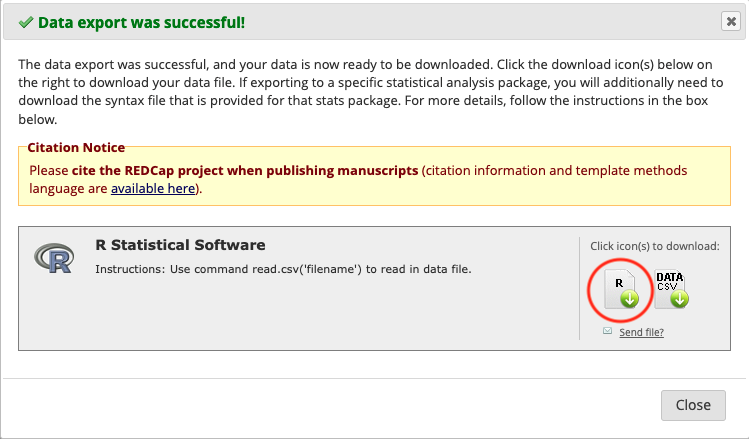
\includegraphics[width=800px]{img/redcap_factoring_file}

Do not click on DATA CSV, because:

\begin{itemize}
\tightlist
\item
  this exact data is already coming via the API pull
\item
  we don't download data onto our computers but pull it directly from REDCap to our secure analysis servers
\end{itemize}

\begin{enumerate}
\def\labelenumi{\arabic{enumi}.}
\setcounter{enumi}{1}
\tightlist
\item
  Move the factoring script to your project directory. The script needs editing to work well with the packages we use. Edit the factoring script as such:
\end{enumerate}

\begin{itemize}
\tightlist
\item
  Delete the first 7 lines.
\item
  Instead, add in
\end{itemize}

\begin{verbatim}
library(finalfit)
library(magrittr)
\end{verbatim}

\begin{enumerate}
\def\labelenumi{\arabic{enumi}.}
\setcounter{enumi}{2}
\item
  Move the labelling section to the bottom of the script. This is because we are about to change it from Hmisc labels to finalfit labels, but the \texttt{factor()} function strips the latter. (Tidyverse functions, on the other hand, strip the former.)
\item
  Change the labels() code from, e.g.,
\end{enumerate}

\begin{verbatim}
label(data$record_id)="Record ID"
label(data$redcap_data_access_group)="Data Access Group"
label(data$sex)="Sex"
label(data$age)="Age"
\end{verbatim}

to

\begin{verbatim}
data$record_id %<>% ff_label("Record ID")
data$redcap_data_access_group %<>% ff_label("Data Access Group")
data$sex %<>% ff_label("Sex")
data$age %<>% ff_label("Age")
\end{verbatim}

Steps:

\begin{itemize}
\tightlist
\item
  Remove \texttt{label(} from the beginning of each line
\item
  Replace \texttt{)=} with \texttt{\%\textless{}\textgreater{}\%\ ff\_label(}
\item
  Complete each line with \texttt{)}
\end{itemize}

Hints and tips:\\
Consider using multiple cursors (click and drag your mouse while holding down Alt on Windows/Linux, or option on a Mac).\\
When doing find and replace, make sure to click ``In selection'' so don't accidentally remove from other sections.\\
For adding \texttt{)} to the end of line, use:


\includegraphics[width=800px]{img/regexp_end_of_line}

\begin{enumerate}
\def\labelenumi{\arabic{enumi}.}
\setcounter{enumi}{4}
\item
  Remove \texttt{.factor} from column names as this creates a duplicate of each column.
\item
  Apply the factoring script on the pulled data: the factoring script assumes the tibble is called \texttt{data}. Instead of going through and changing each instance of this name, do this:
\end{enumerate}

\begin{verbatim}
data = pulled_data
source("REDCap_factoring_script.r")
pulled_data = data
rm(data)
\end{verbatim}

\hypertarget{alternative-to-the-factoring-script-redcap_label-from-librarycollaboratorr}{%
\section{\texorpdfstring{Alternative to the factoring script: \texttt{redcap\_label()} from \texttt{library(collaboratorR)}}{Alternative to the factoring script: redcap\_label() from library(collaboratorR)}}\label{alternative-to-the-factoring-script-redcap_label-from-librarycollaboratorr}}

Optional: \texttt{redcap\_label()} from \texttt{library(collaboratorR)} will do factoring for you by applying information from the project's metadata (which is also pulled via the API). Currently, it uses Hmisc labels so not fully compatible with the tidyverse.

\hypertarget{citations-with-r-markdown}{%
\chapter{Citations with R Markdown}\label{citations-with-r-markdown}}

Writing publications and other documents requires citations both of academic papers and of R packages.

Zotero provides efficient and free reference management which generates new citation objects with the click of a button in Chrome and easy generation of \texttt{.bib} files which can be used to create references in \texttt{rmarkdown} and \texttt{bookdown}.

\emph{Top tip: Do this on Day 1 of your PhD!}

\hypertarget{zotero-set-up}{%
\section{Zotero Set-up}\label{zotero-set-up}}

\href{https://www.zotero.org/download/}{Zotero} should be installed and provides 300MB of free storage which covers a few thousand references as long as PDFs are stored elsewhere. The \href{https://www.zotero.org/download/}{Chrome connector} can be downloaded to allow one-click saving of citations. Just click the icon at the top right of the browser to store meta-data and files.

Set up an online account with Zotero so that your data is available remotely.

\href{https://www.zotero.org/support/plugins}{Zotfile} should be installed to help with PDF storage. Download the \texttt{.xpi} file for Zotfile. To install \textbf{Zotfile} open Zotero and go to \texttt{Tools\ →\ Add-ons\ →\ cog\ in\ top\ right\ corner} and select downloaded \texttt{.xpi} file to install.

\begin{figure}
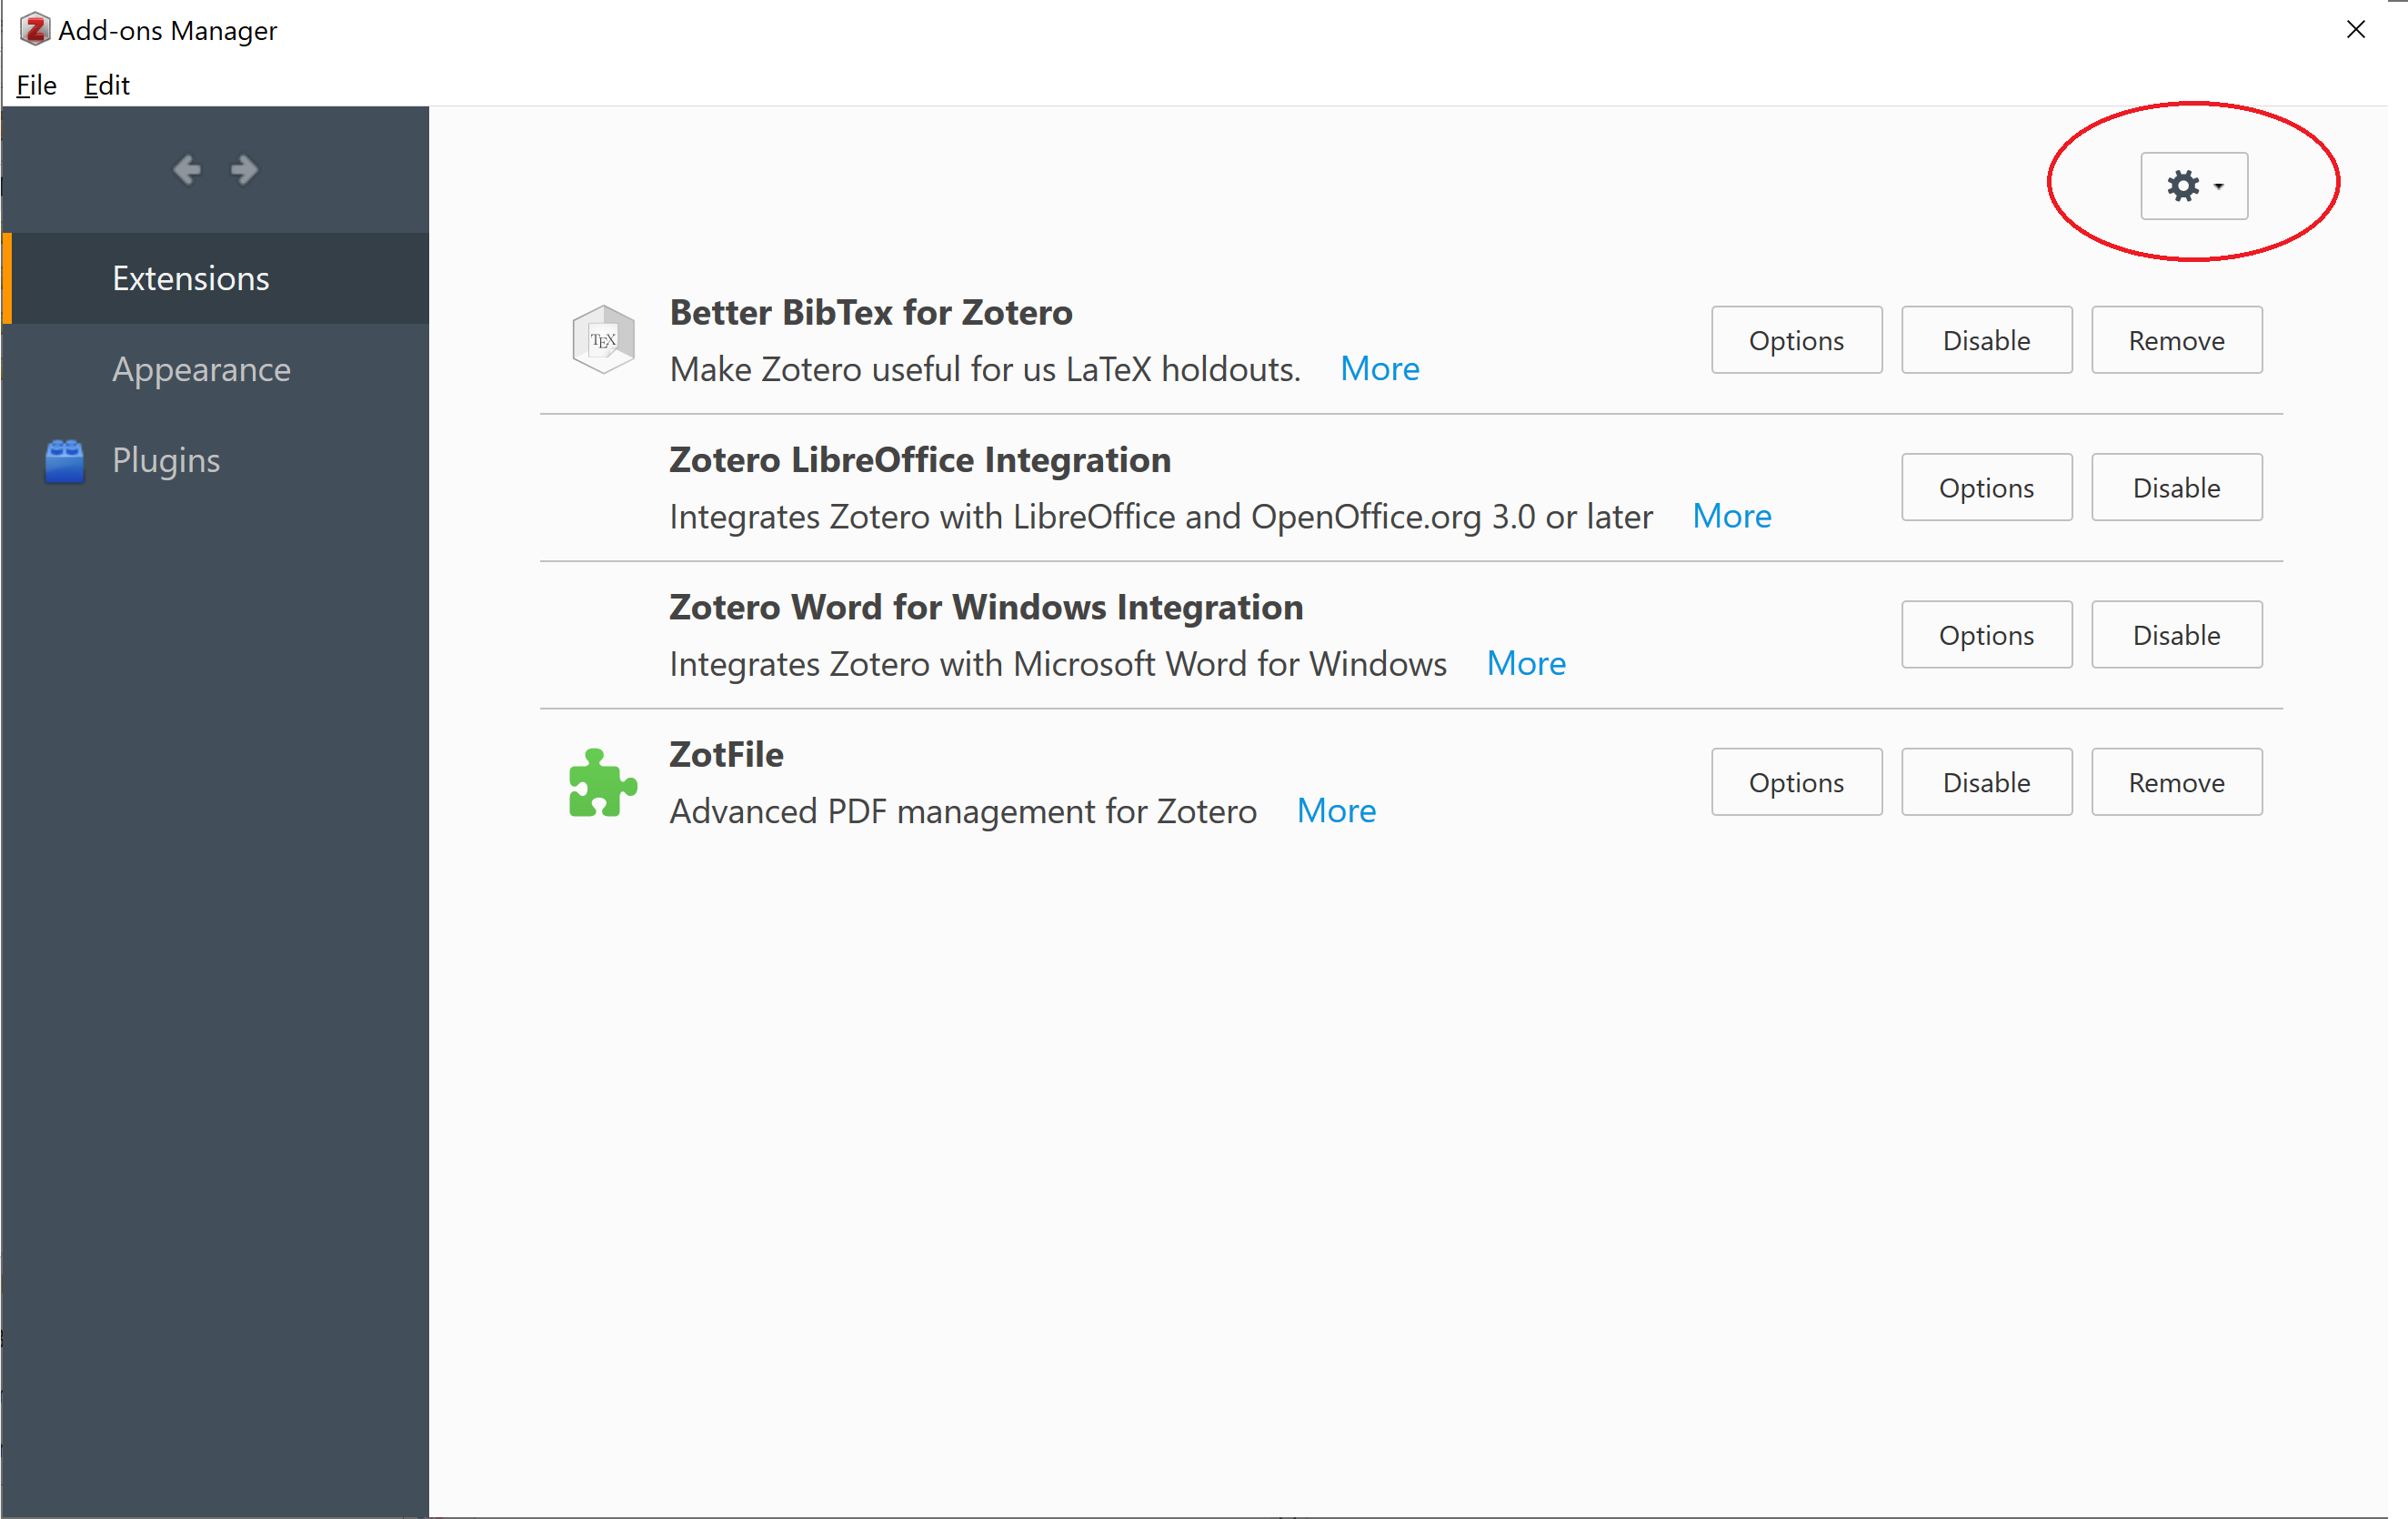
\includegraphics[width=36.78in]{img/zotero_add_on_install} \caption{Installing a Zotero Plug-in from an .xpi File}\label{fig:add-on-install}
\end{figure}

\href{https://github.com/retorquere/zotero-better-bibtex/releases/tag/v5.1.76}{Better BibTeX} is another plug-in which generates citation keys in a robust and reproducible way which is needed for larger projects (e.g.~PhDs) to avoid duplicate citation handles. An \texttt{.xpi} file can be downloaded from GitHub and installed in the same way.

\hypertarget{file-storage-set-up}{%
\section{File Storage Set-up}\label{file-storage-set-up}}

In addition to Zotero set-up it is a good idea to have a cloud storage service to maintain a library of PDFs without using up Zotero storage capacity. These will also need to be accessible to the \texttt{Windows\ Explorer} or the \texttt{Mac\ Finder} - there are several guides on how to do this for \href{https://www.howtogeek.com/228989/how-to-use-the-desktop-google-drive-app/}{Google Drive} and \href{https://www.dropboxforum.com/t5/Installation-and-desktop-app/How-do-I-put-Dropbox-on-my-File-Explorer-in-Win-10/td-p/313031}{DropBox}.

\hypertarget{folder-set-up}{%
\section{Folder Set-up}\label{folder-set-up}}

\hypertarget{storing-pdfs}{%
\subsection{Storing PDFs}\label{storing-pdfs}}

Create a folder in a cloud storage service to store PDFs which can be accessed from your own file explorer.

\hypertarget{storing-bibliographies}{%
\subsection{Storing Bibliographies}\label{storing-bibliographies}}

Create a folder which will store your \texttt{.bib} file. This can then be used to provide the references for your \texttt{.rmd} files.

\hypertarget{subfolder-for-references}{%
\subsection{Subfolder for References}\label{subfolder-for-references}}

It may be a good idea in Zotero to carefully categorise publications by their content. This makes it very easy to look up publications on a given topic (Zotero allows a citation to be shared across several folders such that a publication documenting an RCT with updated meta-analysis could be in folders for each type of study etc.).

Generally a parent folder will be used to generate a bibliography file and anything likely to be cited in a document / thesis should be in that folder or one of its subfolders.

\hypertarget{configuring-zotero}{%
\section{Configuring Zotero}\label{configuring-zotero}}

\hypertarget{zotfile-pdf-preferences}{%
\subsection{ZotFile PDF Preferences}\label{zotfile-pdf-preferences}}

To setup Zotero so that retrieved PDFs are automatically stored and renamed in the cloud storage without consuming the Zotero storage quota go to ``Tools → ZotFile Preferences'' and on the first tab: \textbf{General Settings} and set the folder and subfolder naming strategy for PDFs. Set the location of the files to a Custom location in cloud storage e.g.(``\textasciitilde\textbackslash Google Drive\textbackslash Zotero PDF Library''). ZotFile will also store retrieved PDFs in subfolders to help with finding PDFs at a later date. A reasonable setup is to create a subfolder with the first author surname so that all papers authored by one (or more) author with the same name are stored together using the \textbackslash\%a in the subfolder field. Other alternatives are to store PDFs in subfolders using year (\textbackslash\%y); journal or publisher (\textbackslash\%w); or item type (\textbackslash\%T).

\begin{figure}
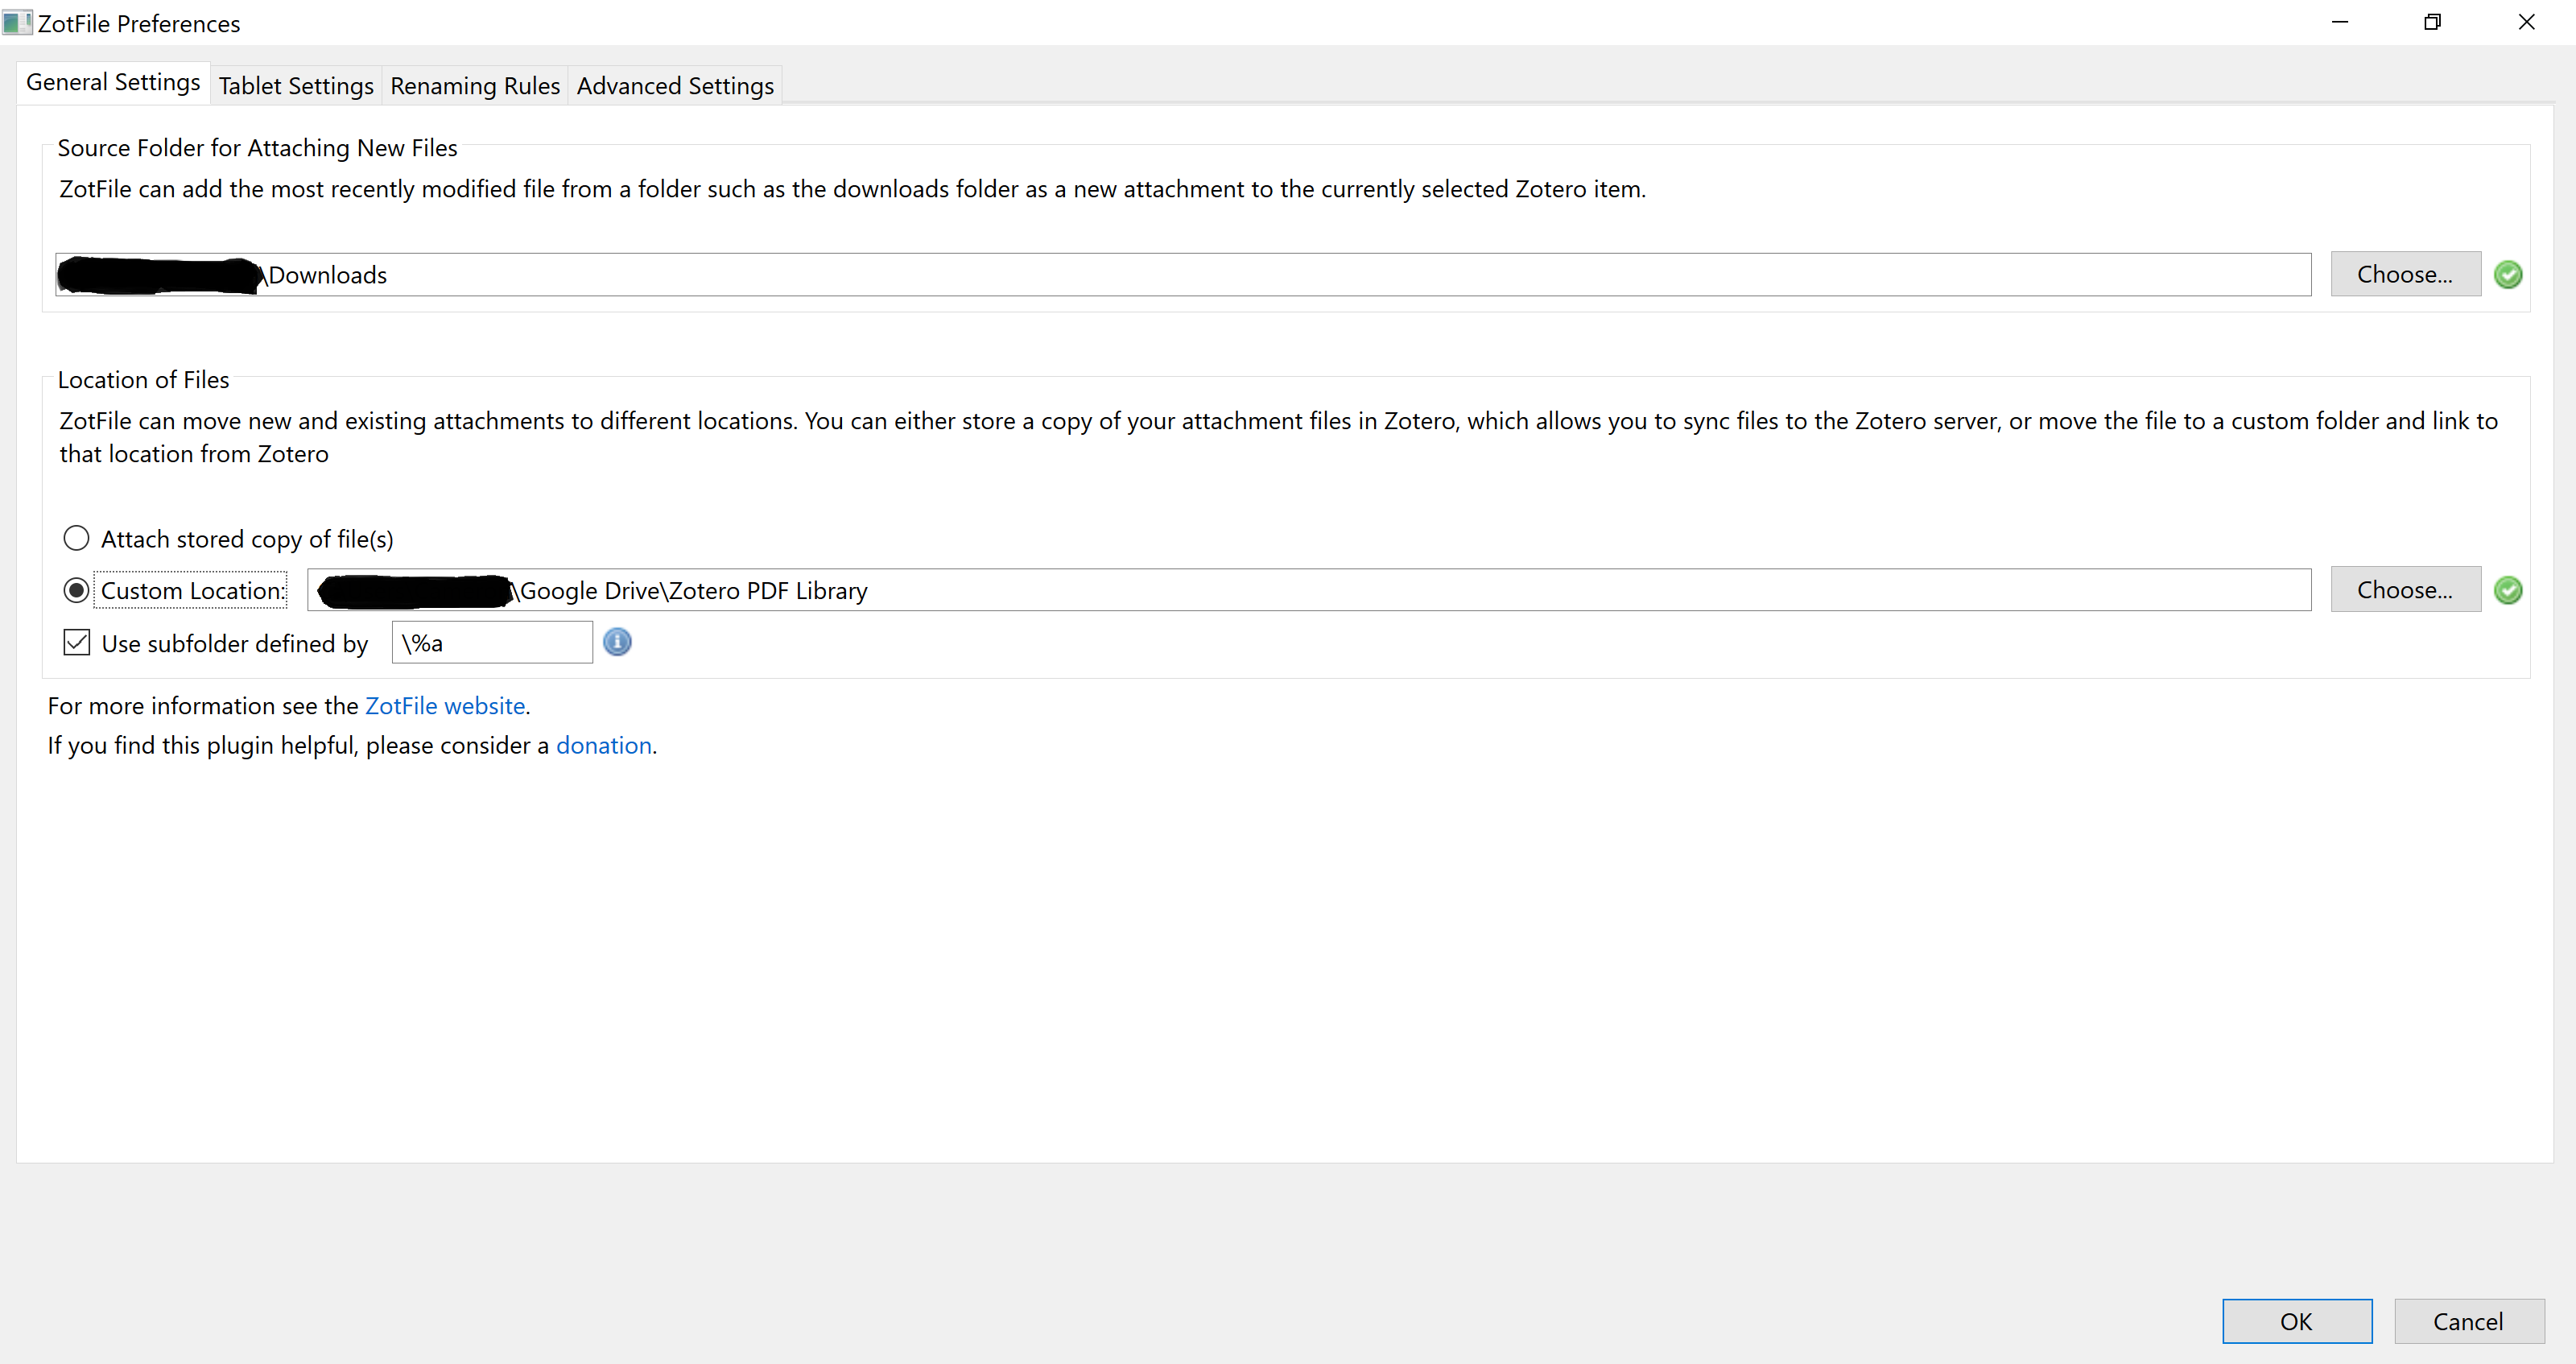
\includegraphics[width=44.44in]{img/zotfile_preferences} \caption{ZotFile PDF Storage Preferences}\label{fig:zotfile-preferences}
\end{figure}

Next the \textbf{Renaming Rules} tab can be configured to provide sensible names to each of the files (this is essential if PDFs are not to be stored as random strings of characters which provide no meaning). Setting the format to: \{\%a\_\}\{\%y\_\}\{\%t\} provides names for the PDFs in the format of: \texttt{Fairfield\_2019\_Gallstone\_Disease\_and\_the\_Risk\_of\_Cardiovascular\_Disease.pdf}. This shows author, year and first word of title without needing to expand the file name.

\begin{figure}
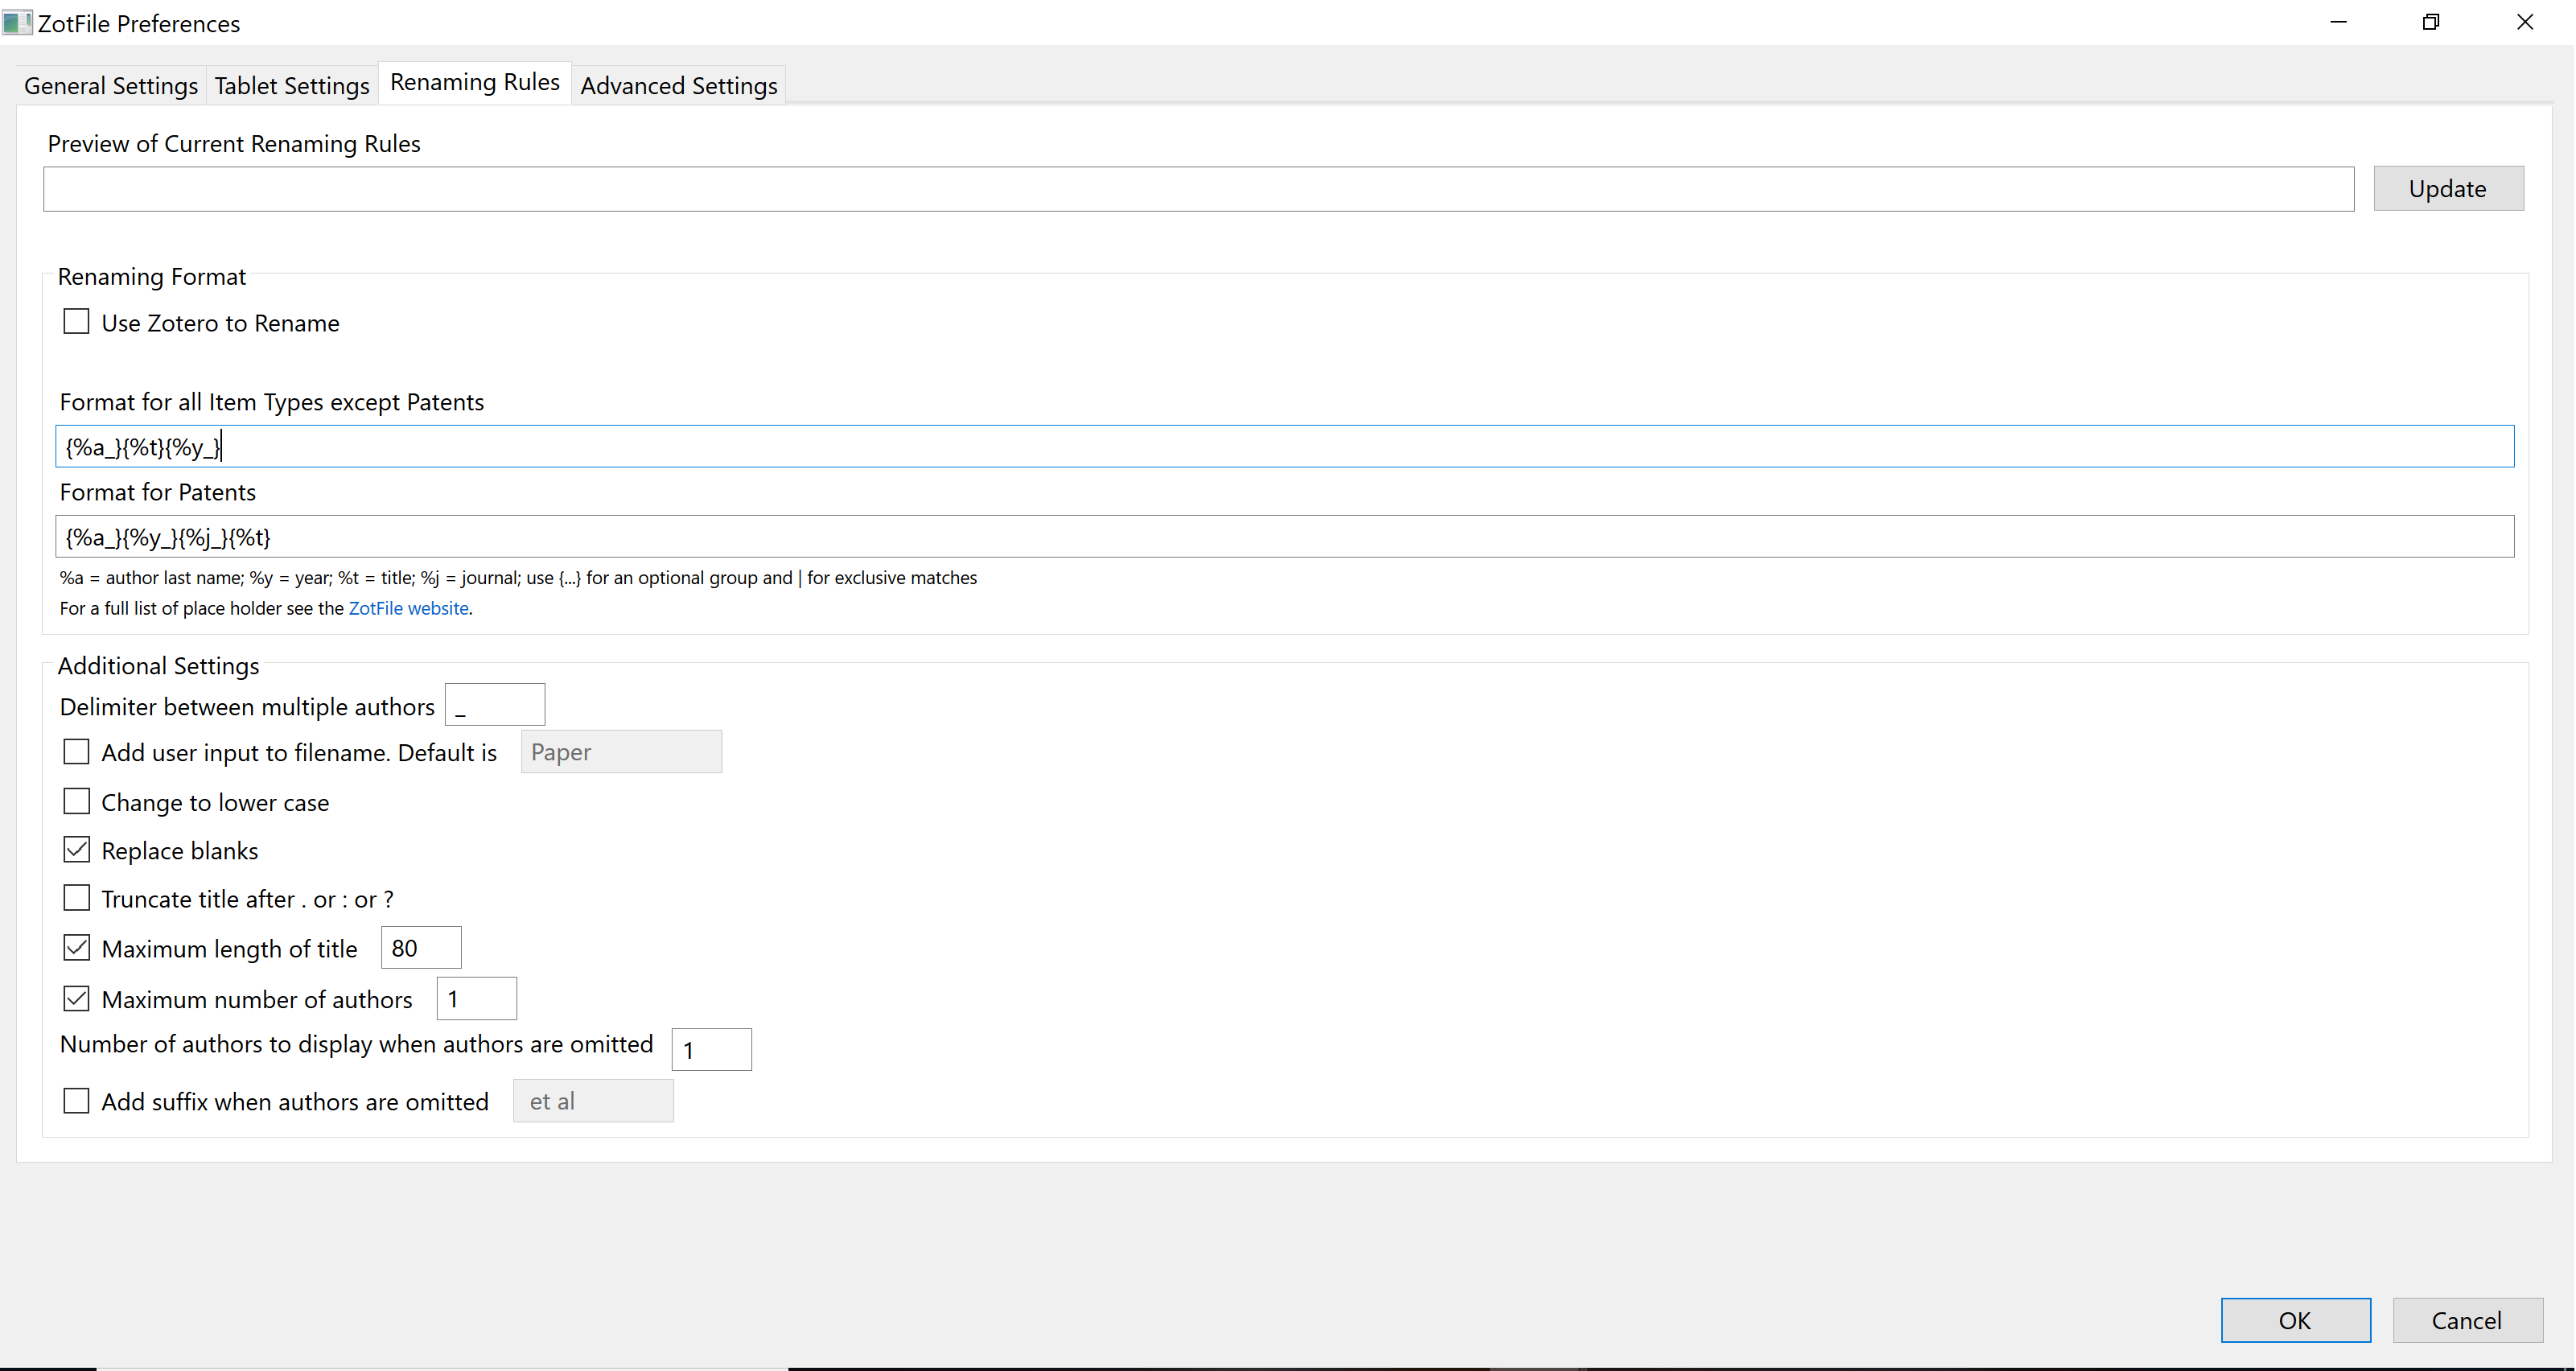
\includegraphics[width=44.47in]{img/zotfile_renaming} \caption{ZotFile PDF Storage Preferences}\label{fig:zotfile-renaming}
\end{figure}

In the \textbf{Advanced Settings} tab it is strongly recommended to select removal of ``Special characters'', leaving these in creates problems when knitting to PDF as LaTeX may recognise the special characters in unexpected ways.

\hypertarget{general-zotero-settings}{%
\subsection{General Zotero Settings}\label{general-zotero-settings}}

Zotero has several configurable settings (accessed through: ``Edit → Preferences''). The following settings are generally helpful (left as default if not mentioned):

\textbf{General:}
+ Tick the following:
+ Automatically attach associated PDFs
+ Automatically retrieve metadata for PDFs
+ Automatically rename attachments using parent metadata
+ Automatically tag items with keywords and subject headings
+ All options in Group section
+ Leave the following unticked:
+ Automatically take snapshots
+ Rename linked files

\textbf{Sync:}
+ Enter the account details
+ Tick sync automatically
+ Untick sync full text (if you choose to save PDFs then syncing full text will quickly consume the 300MB quota)

\textbf{Search:}
+ Leave unchanged

\textbf{Export:}
+ Leave unchanged

\textbf{Cite:}
+ There are several sensible defaults but if there is a new citation style you wish to be able to use in Microsoft Word for example then click ``Get additional styles'' as there is probably a version that you need already created. You can click the ``+'' button to add a style from a \texttt{.csl} file if you have one already. Finally, if you are desperate for a style that doesn't already exist then you can select a citation style and click Style Editor and edit the raw \texttt{.csl} file. The \texttt{.csl} file for use in \texttt{.rmd} doesn't need configured here but instead within the YAML of your .rmd file
+ In the Word Processors subtab (on the main Cite tab), you can install the Microsoft Word add-in to allow Zotero to work in Microsoft Word.

\textbf{Advanced:}
+ Change nothing on the General subtab
+ In the Files and Folders subtab select the path to directory for attachments
+ Change nothing on the Shortcuts subtab
+ Change nothing on the Feeds subtab

\textbf{Better BibTex:}
+ In this section set the Citation Key format to {[}auth:lower:alphanum{]}\emph{{[}year:alphanum{]}}{[}veryshorttitle:lower:alphanum{]}\_{[}journal:lower:clean:alphanum{]} (Figure 4). This generates a citation key for each reference in the format of fairfield\_2019\_gallstones\_scientificreports or harrison\_2012\_hospital\_bmj. It always takes the first author's surname, the year, the first word of the title and the journal abbreviation if known. The clean and alphanum arguments to this field are used to remove unwanted punctuation which can cause citation to fail in LaTeX.

If an author has published an article with the same first word of the title in the same year then the second article appends an ``a'' to the handle and the third a ``b'' and so on.

\begin{figure}
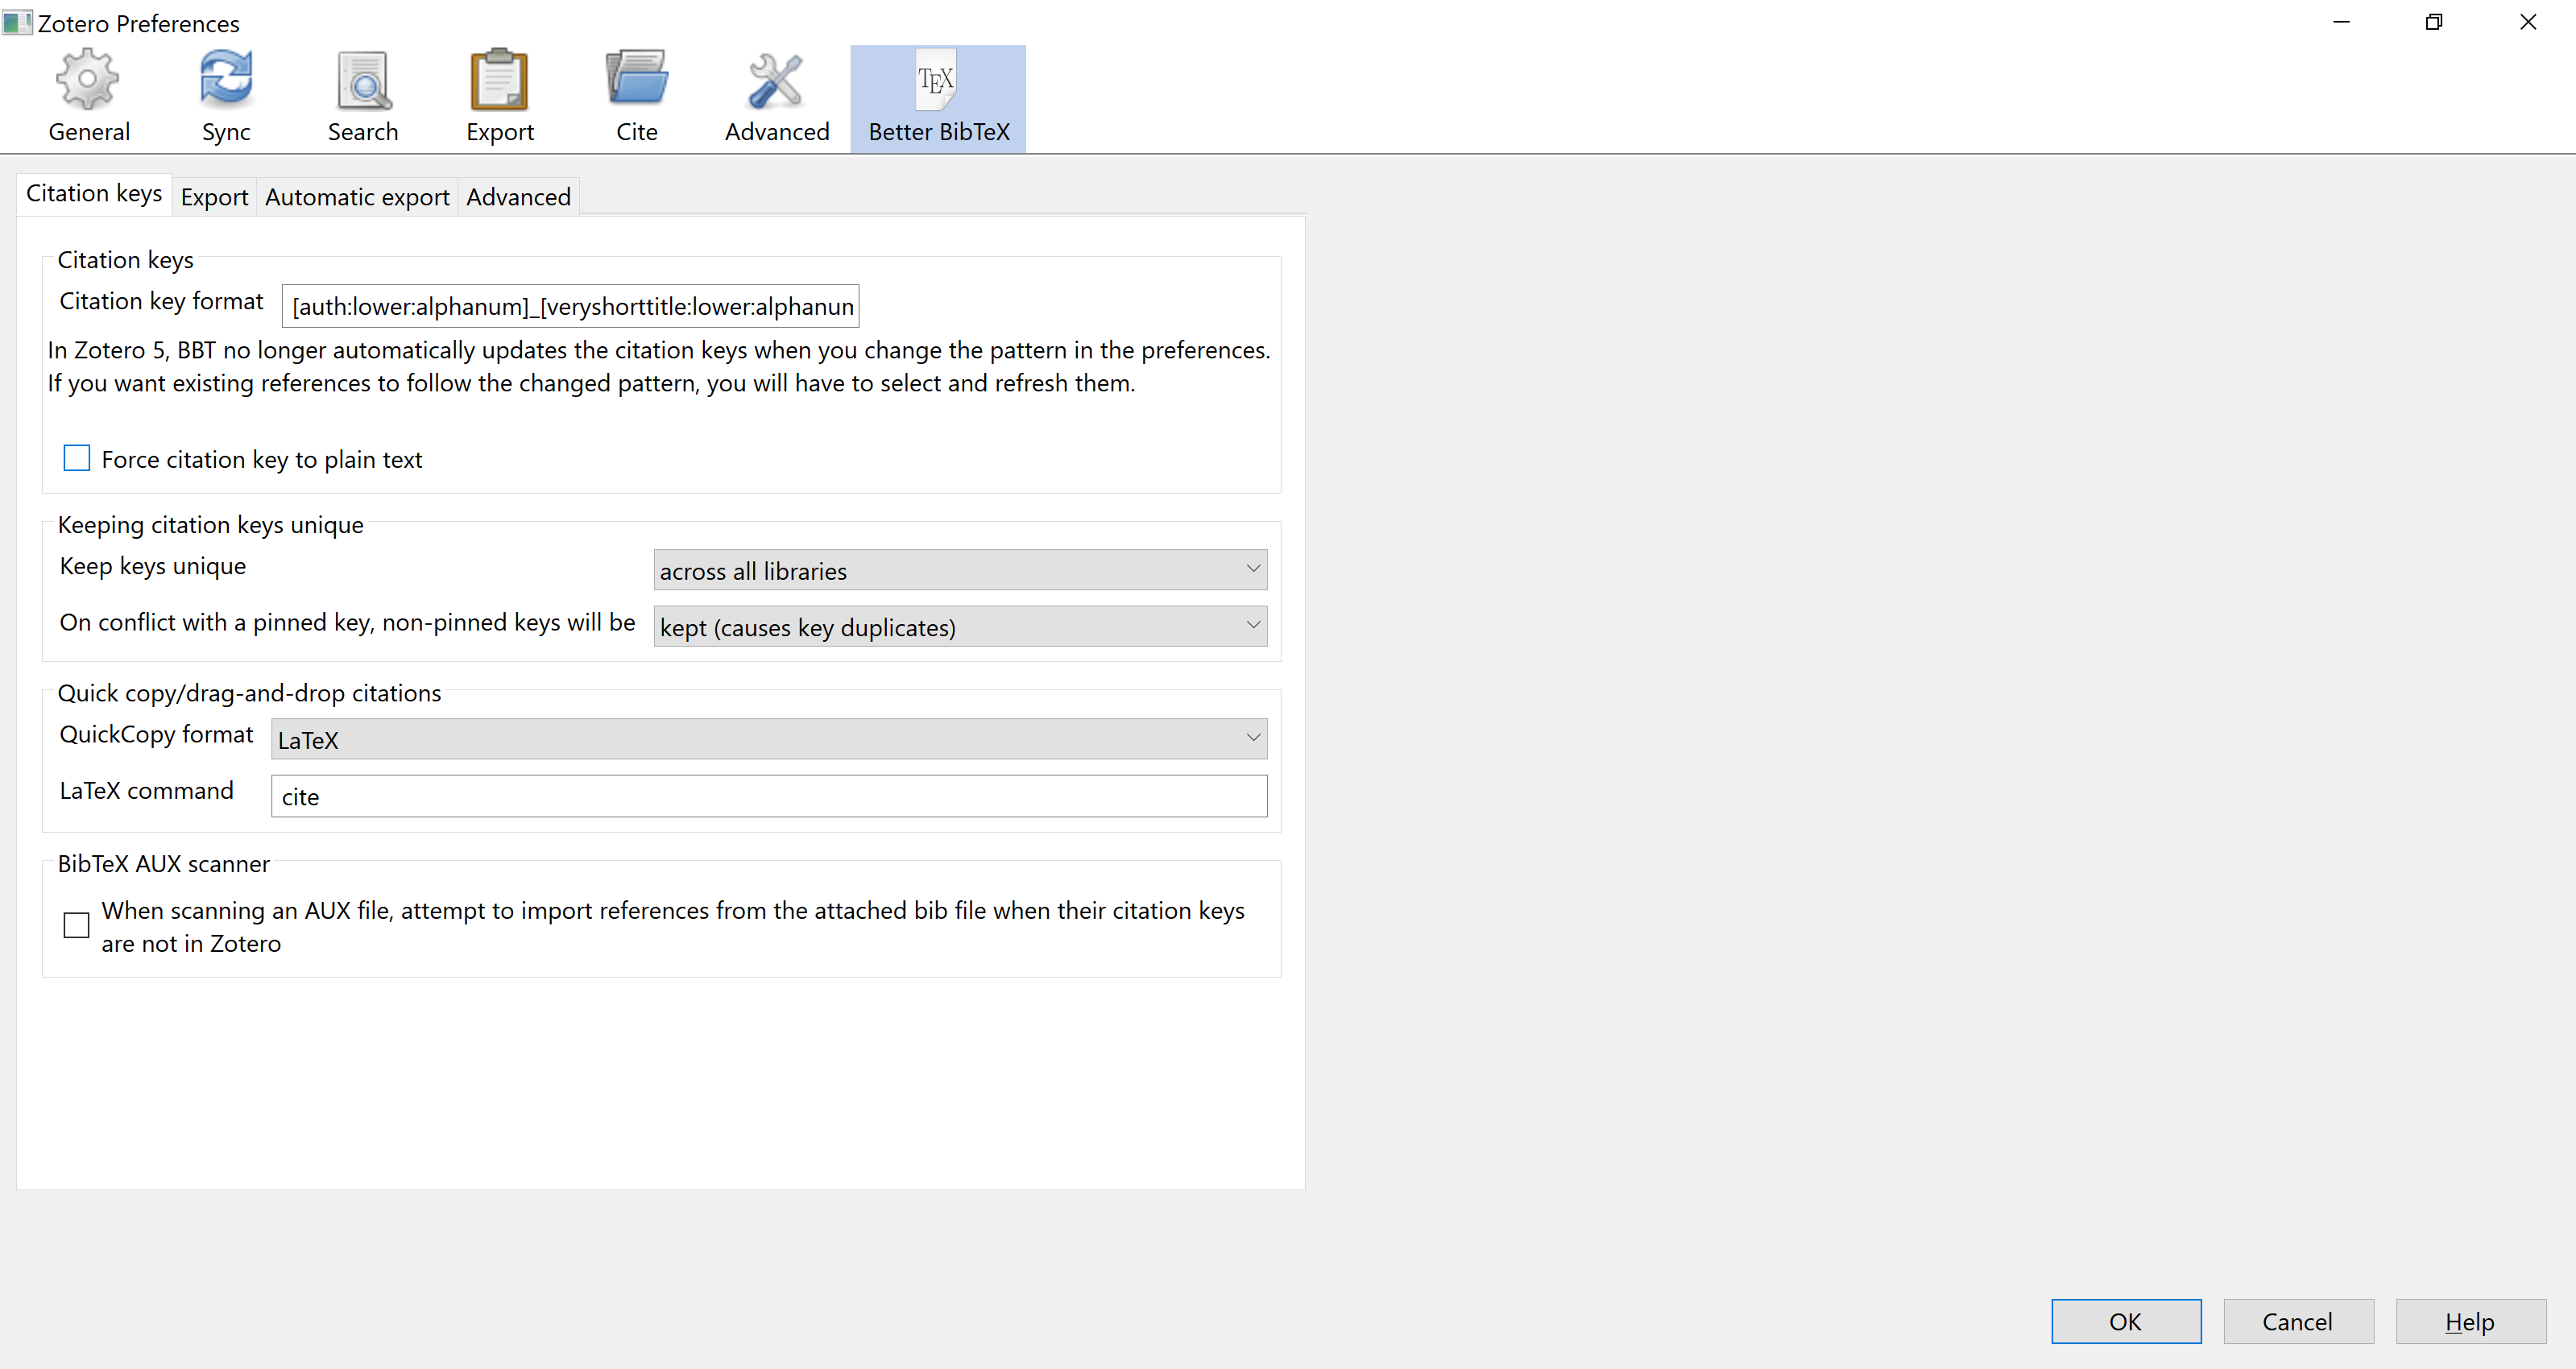
\includegraphics[width=44.42in]{img/zotero_citation_key} \caption{ZotFile PDF Storage Preferences}\label{fig:zotfile-citation-key}
\end{figure}

\hypertarget{refresh-bibtex-citation-key}{%
\subsection{Refresh BibTex Citation Key}\label{refresh-bibtex-citation-key}}

If you already have used Zotero without this setup and want to refresh your citation keys to follow the standard pattern then select all references, right click and use ``Better BibTex → Refresh BibTeX Key''.

\hypertarget{generating-a-.bib-file}{%
\section{Generating a .bib File}\label{generating-a-.bib-file}}

For referencing in a new project, publication or submission it may be helpful to have a dynamic \texttt{.bib} file that updates with every new publication added to Zotero and can be accessed from any device through cloud storage.

To set up a \texttt{.bib} file, first find the folder that you wish to create the file from (this should be the folder which contains any citations you will use and ideally not the full library to cut down on unnecessary storage and syncing requirements).

Note that the \texttt{.bib} file will generate a bibliography from any citations stored directly in the folder when using default settings. This prevents use of subfolders which are particularly helpful for organising citations so it may be helpful to change the setting so that folders also show any citations stored in subfolders. To make this change go to ``Edit Preferences'' and select the ``Advanced'' tab and at the bottom of the ``General'' subtab select ``Config Editor''. This will bring up a searchable list of configurations (it may show a warning message before this) and search in the search box for ``extensions.zotero.recursiveCollections''. Set ``Value'' to TRUE and then when you click a folder you should see all of the citations also stored in subfolders.

Right click the folder which has all of the references (with or without subfolders) and select ``Export Collection''. A pop-up window will appear at which point select ``Keep Updated'' and if using RStudio desktop save the file in the directory where you have your \texttt{.rmd} project files. If you are working with RStudio server then save the file in a cloud storage location which will then be accessed from the server. A \texttt{.bib} file stored in Dropbox can be copied into RStudio server for a given project as per below.

\hypertarget{linking-dropbox-and-rstudio-server}{%
\section{Linking DropBox and Rstudio Server}\label{linking-dropbox-and-rstudio-server}}

Dropbox provides a token to allow communication between different apps. The \texttt{rdrop2} package allows this. It may be necessary to create the token on RStudio desktop as creation on the server is buggy but this is perfectly ok.

\textbf{Caution:} The token generated by this process could be used to access your Dropbox from anywhere using RStudio if you do not keep it secure. If somebody were to access an unencrypted token then it would be equivalent to handing out your email and password. Use the \texttt{encryptr} package to allow safe storage of this token.

\hypertarget{token-creation}{%
\subsection{Token Creation}\label{token-creation}}

The code will create two files, a token and the \texttt{.httr-oauth} file from which a token can also be made. The encryptr package can then encrypt the files using a public / private key pair. It is essential that the password that is set when using genkeys() is remembered otherwise the token cannot then be used. In this case the original token can't be retrieved but could be created again from scratch.

\begin{Shaded}
\begin{Highlighting}[]
\FunctionTok{library}\NormalTok{(rdrop2)}
\FunctionTok{library}\NormalTok{(encryptr)}
 
\CommentTok{\# Create token}
\NormalTok{token }\OtherTok{\textless{}{-}} \FunctionTok{drop\_auth}\NormalTok{()}
 
\CommentTok{\# Save token}
\FunctionTok{saveRDS}\NormalTok{(token, }\StringTok{"droptoken.rds"}\NormalTok{)}
 
\CommentTok{\# Encrypt token}
\FunctionTok{genkeys}\NormalTok{()               }\CommentTok{\# Default file names are id\_rsa and id\_rsa.pub}
\FunctionTok{encrypt\_file}\NormalTok{(}\StringTok{"droptoken.rds"}\NormalTok{, }\StringTok{"droptoken.rds.encryptr.bin"}\NormalTok{)}
\FunctionTok{encrypt\_file}\NormalTok{(}\StringTok{".httr{-}oauth"}\NormalTok{, }\StringTok{".httr{-}oauth.encryptr.bin"}\NormalTok{)}
 
\CommentTok{\# Same details should appear later}
\FunctionTok{drop\_acc}\NormalTok{()}
 
\CommentTok{\# Remove token from local environment}
\FunctionTok{rm}\NormalTok{(token)}
 
 
\CommentTok{\# Delete the unencrypted files}
\FunctionTok{system}\NormalTok{(}\StringTok{"rm droptoken.rds"}\NormalTok{)}
\FunctionTok{system}\NormalTok{(}\StringTok{"rm .httr{-}oauth"}\NormalTok{)}
\end{Highlighting}
\end{Shaded}

The following files will then be needed to upload to the RStudio server:

\begin{itemize}
\tightlist
\item
  \texttt{droptoken.rds.encryptr.bin} -- or the name provided for the encrypted DropBox token
\item
  \texttt{id\_rsa} -- or the name provided for the private key from the private / public key pair
\end{itemize}

\hypertarget{dropbox-linkage}{%
\subsection{DropBox Linkage}\label{dropbox-linkage}}

Now that the encrypted token and necessary (password-protected) private key are available in RStudio server, the following can be saved as a separate script. The script is designed to read in and decrypt the encrypted token (this will require a password and should be done if the .bib file needs updated). Only the drop\_download() needs repeated if using the token again during the same session. The token should be cleared at the end of every session for additional security.

\begin{Shaded}
\begin{Highlighting}[]
\FunctionTok{library}\NormalTok{(rdrop2)}
\FunctionTok{library}\NormalTok{(encryptr)}
 
\CommentTok{\# ******** }\AlertTok{WARNING}\CommentTok{ ********}
\CommentTok{\# Losing the unencrypted token will give anyone }
\CommentTok{\# complete control of your Dropbox account}
\CommentTok{\# If you are concerned this has happened,}
\CommentTok{\# you can then revoke the rdrop2 app from your}
\CommentTok{\# dropbox account and start over.}
\CommentTok{\# ******** }\AlertTok{WARNING}\CommentTok{ ********}
 
 
\NormalTok{safely\_extract\_dropbox\_token }\OtherTok{\textless{}{-}} \ControlFlowTok{function}\NormalTok{(}\AttributeTok{encrypted\_db\_token =} \ConstantTok{NULL}\NormalTok{, }
                                         \AttributeTok{private\_key\_file =} \ConstantTok{NULL}\NormalTok{)\{}
  \FunctionTok{decrypt\_file}\NormalTok{(encrypted\_db\_token, }
               \AttributeTok{file\_name =} \StringTok{"temporary\_dropbox\_token.rds"}\NormalTok{, }
               \AttributeTok{private\_key\_path =}\NormalTok{ private\_key\_file)}
  
\NormalTok{  token }\OtherTok{\textless{}\textless{}{-}} \FunctionTok{readRDS}\NormalTok{(}\StringTok{"temporary\_dropbox\_token.rds"}\NormalTok{)}
  
  \FunctionTok{system}\NormalTok{(}\StringTok{"rm temporary\_dropbox\_token.rds"}\NormalTok{)}
\NormalTok{\}}
 
\FunctionTok{safely\_extract\_dropbox\_token}\NormalTok{(}\AttributeTok{encrypted\_db\_token =} \StringTok{"droptoken.rds.encryptr.bin"}\NormalTok{, }
                             \AttributeTok{private\_key\_file =} \StringTok{"id\_rsa"}\NormalTok{)}
 
\CommentTok{\# Then pass the token to each drop\_ function}
\FunctionTok{drop\_acc}\NormalTok{(}\AttributeTok{dtoken =}\NormalTok{ token)}
 
\CommentTok{\# The path is the Dropbox file location}
\FunctionTok{drop\_download}\NormalTok{(}\AttributeTok{path =} \StringTok{"My\_Dropbox\_Home\_Directory/Zotero Library/my.bib"}\NormalTok{, }
              \AttributeTok{local\_path =} \StringTok{"my.bib"}\NormalTok{, }
              \AttributeTok{dtoken =}\NormalTok{ token,}
              \AttributeTok{overwrite =} \ConstantTok{TRUE}\NormalTok{)}
\end{Highlighting}
\end{Shaded}

Now that the \texttt{.bib} file has been created and is stored as ``my.bib'' in the local directory, it should update whenever the token is loaded and drop\_download() is run. The \texttt{.bib} file should be listed in the \texttt{.rmd} YAML.

\hypertarget{citing-r-packages}{%
\section{Citing R Packages}\label{citing-r-packages}}

When citing R packages a separate \texttt{.bib} file can be created. The following code could be added to an \texttt{index.rmd} file in \texttt{bookdown} or in a setup chunk in a stand-alone \texttt{.rmd}.

\begin{Shaded}
\begin{Highlighting}[]
\CommentTok{\# automatically create a bib database for R packages}
\NormalTok{knitr}\SpecialCharTok{::}\FunctionTok{write\_bib}\NormalTok{(}\FunctionTok{c}\NormalTok{(}
  \FunctionTok{.packages}\NormalTok{(), }\StringTok{\textquotesingle{}encryptr\textquotesingle{}}\NormalTok{, }\StringTok{\textquotesingle{}knitr\textquotesingle{}}\NormalTok{, }\StringTok{\textquotesingle{}rmarkdown\textquotesingle{}}
\NormalTok{), }\StringTok{\textquotesingle{}packages.bib\textquotesingle{}}\NormalTok{)}
\end{Highlighting}
\end{Shaded}


  \bibliography{book.bib,packages.bib}

\end{document}
